\begin{figure}[!htb]
	\begin{center}
  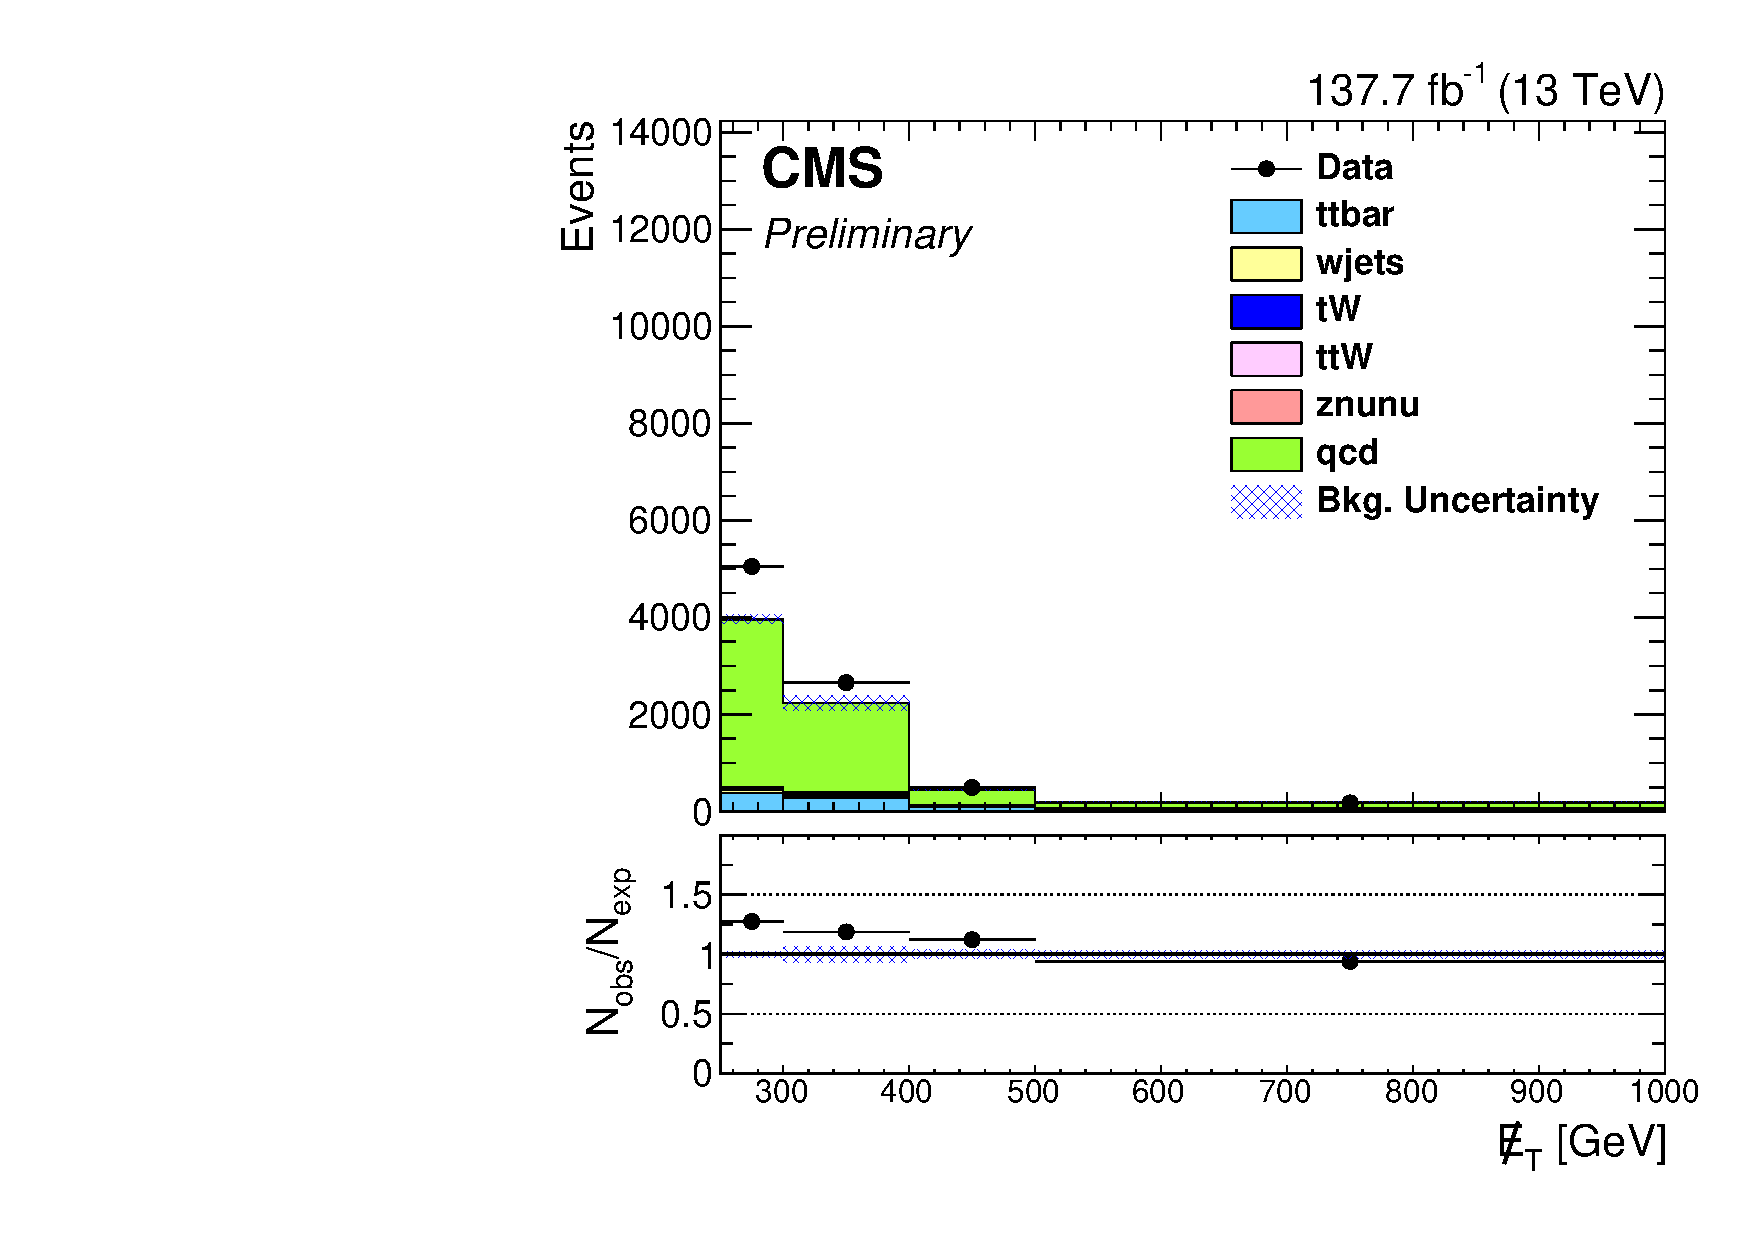
\includegraphics[width=0.32\textwidth]{../Research/SUSY/2019/LLB/lepcr_allEras/MET_pt_DataMC_hm_nb1_lowmtb_nj7_nrtgeq1__.pdf}
  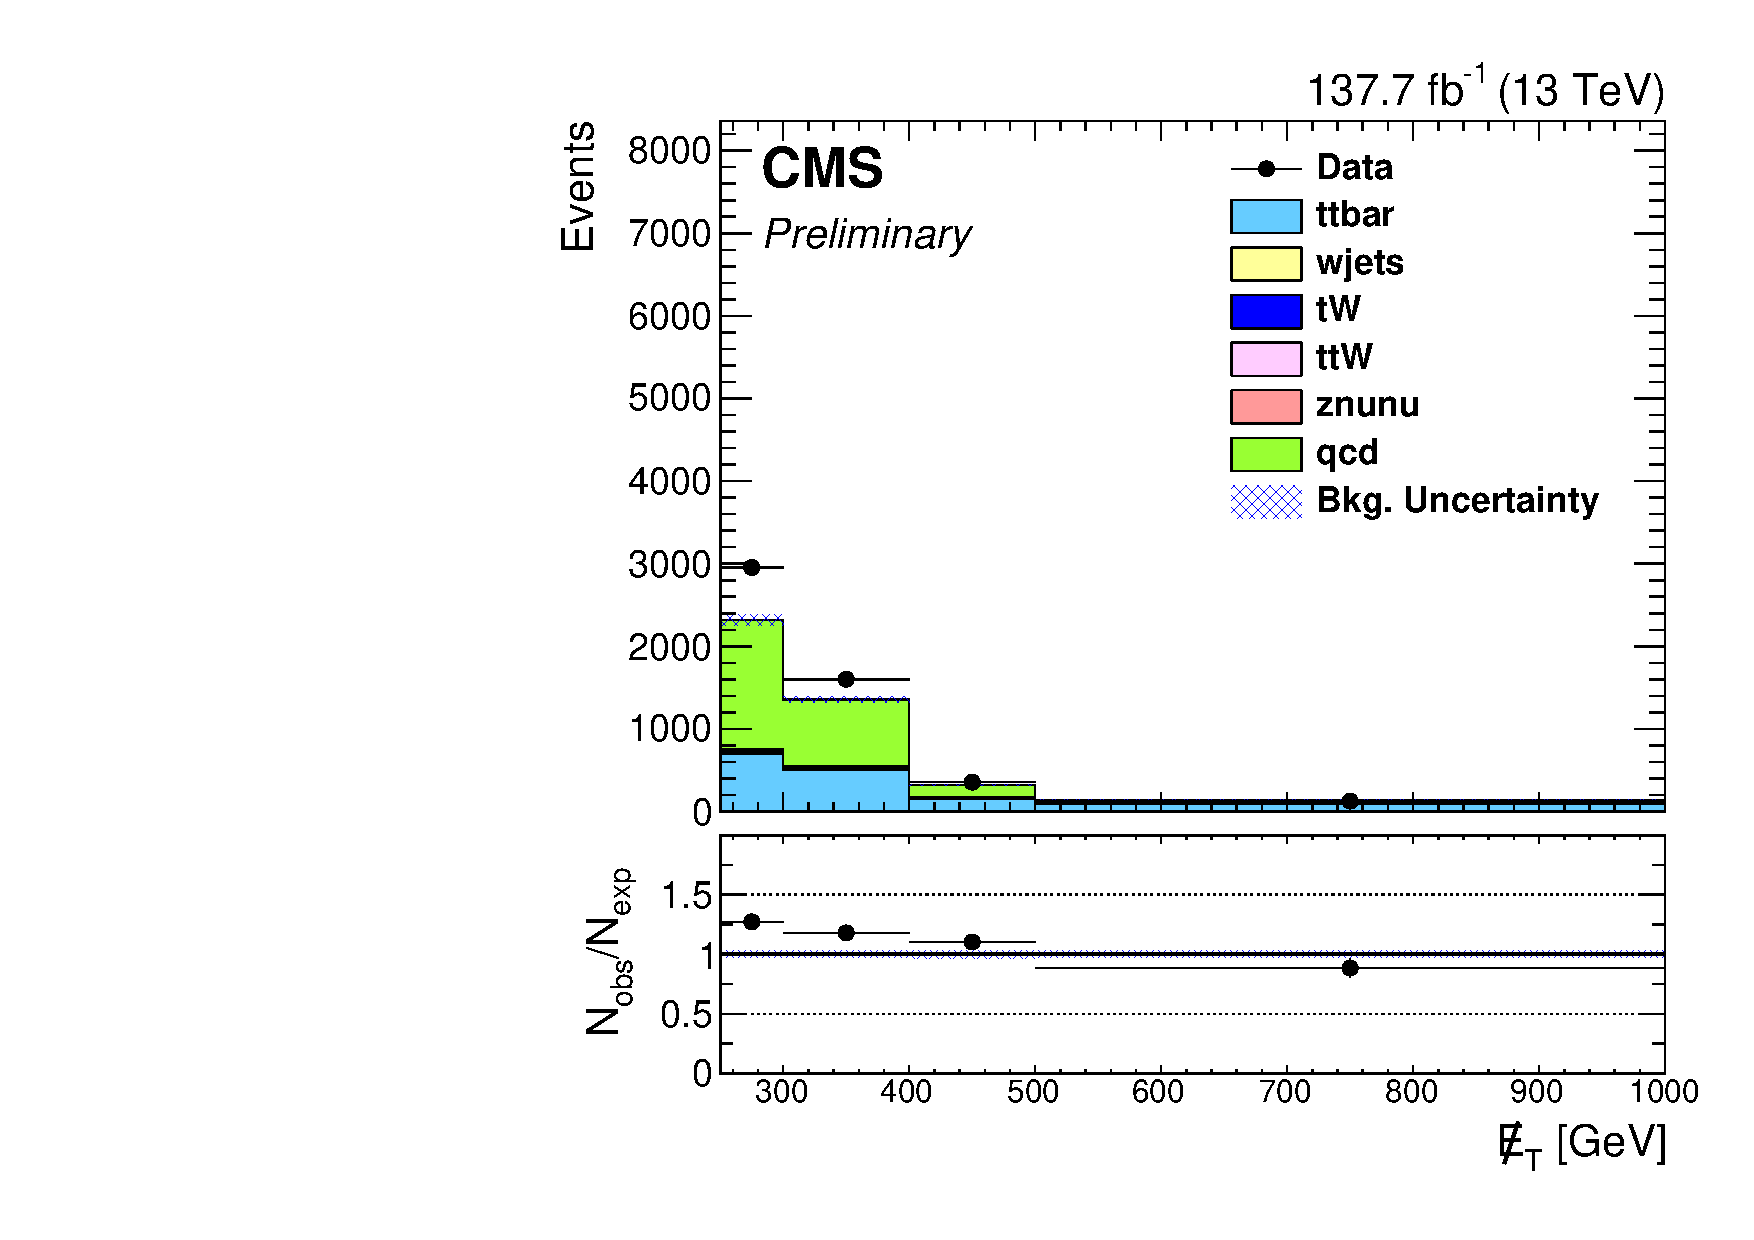
\includegraphics[width=0.32\textwidth]{../Research/SUSY/2019/LLB/lepcr_allEras/MET_pt_DataMC_hm_nb2_lowmtb_nj7_nrtgeq1__.pdf} \\
  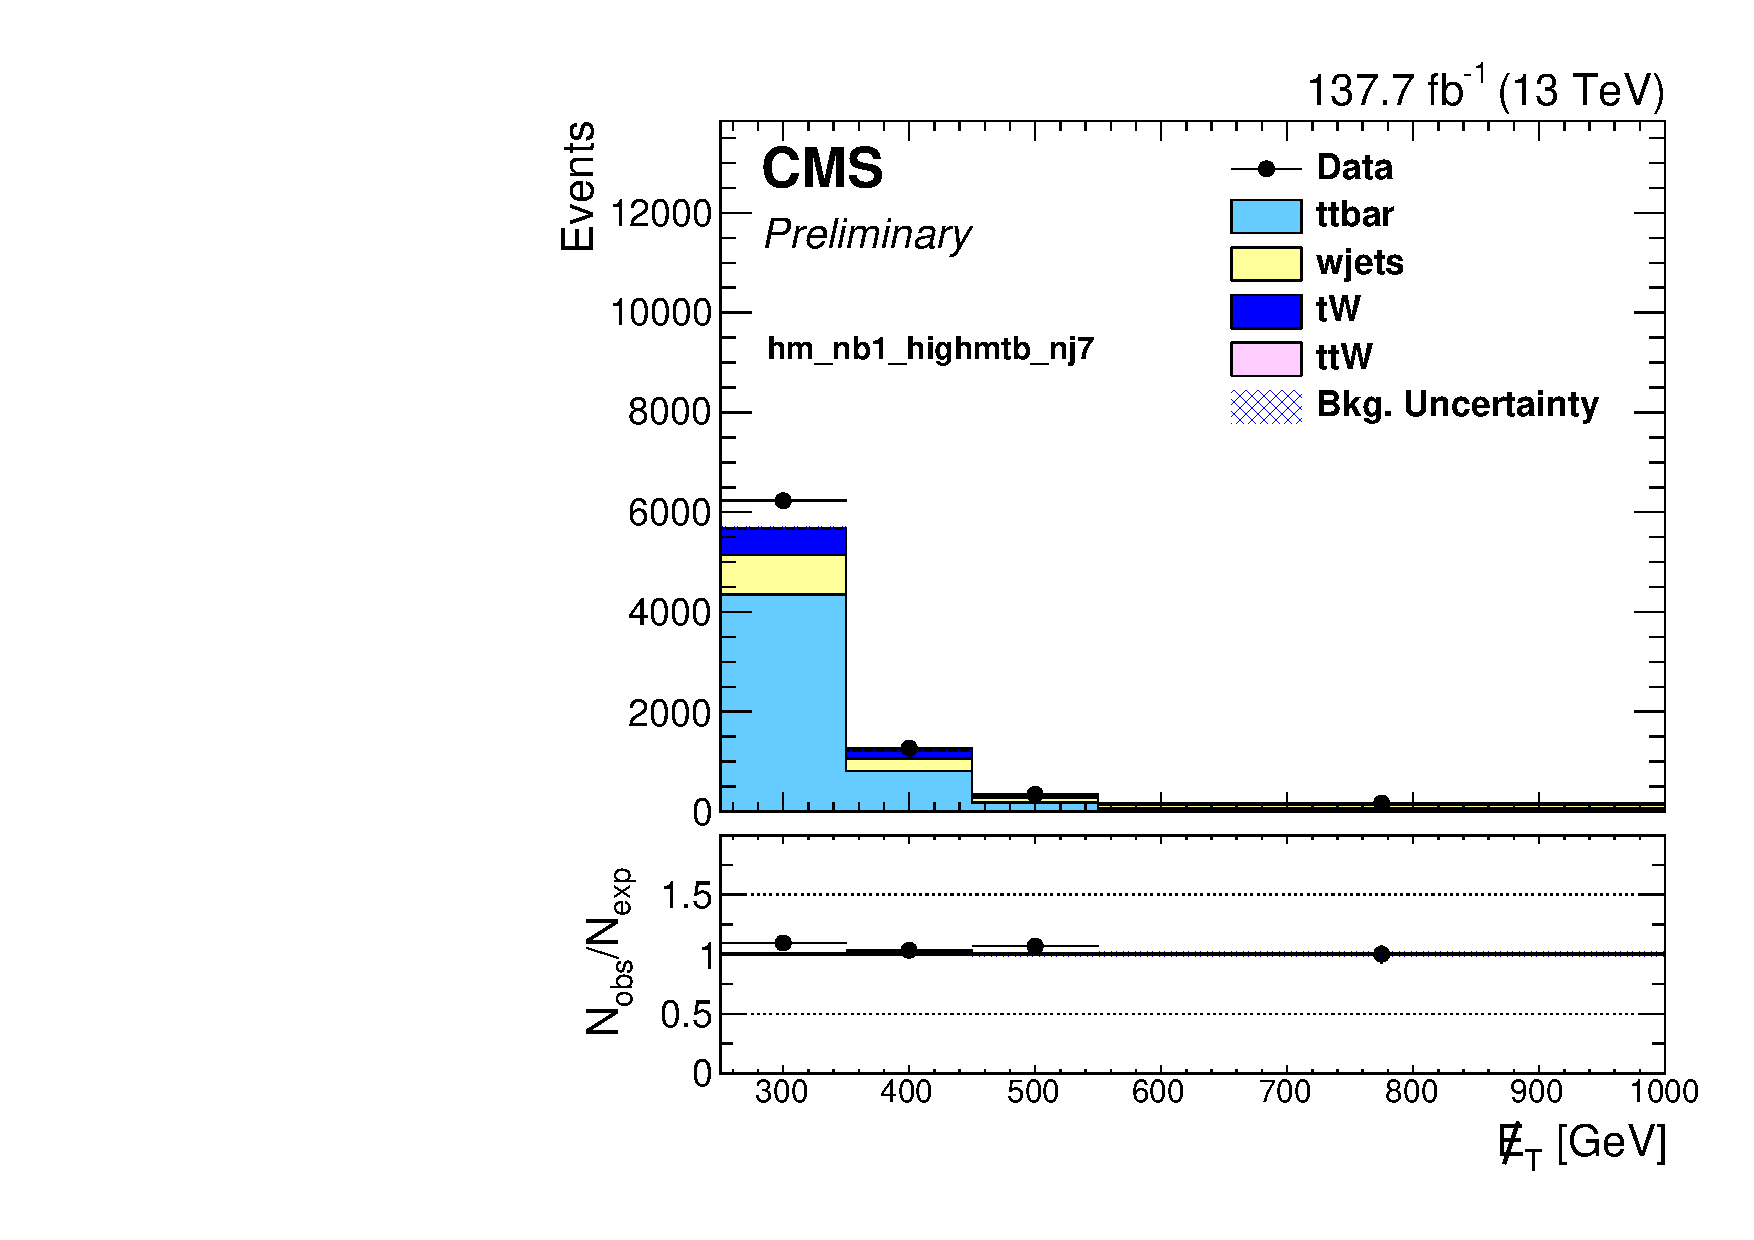
\includegraphics[width=0.32\textwidth]{../Research/SUSY/2019/LLB/lepcr_allEras/MET_pt_DataMC_hm_nb1_highmtb_nj7_nt0_nrt0_nw0__.pdf}
  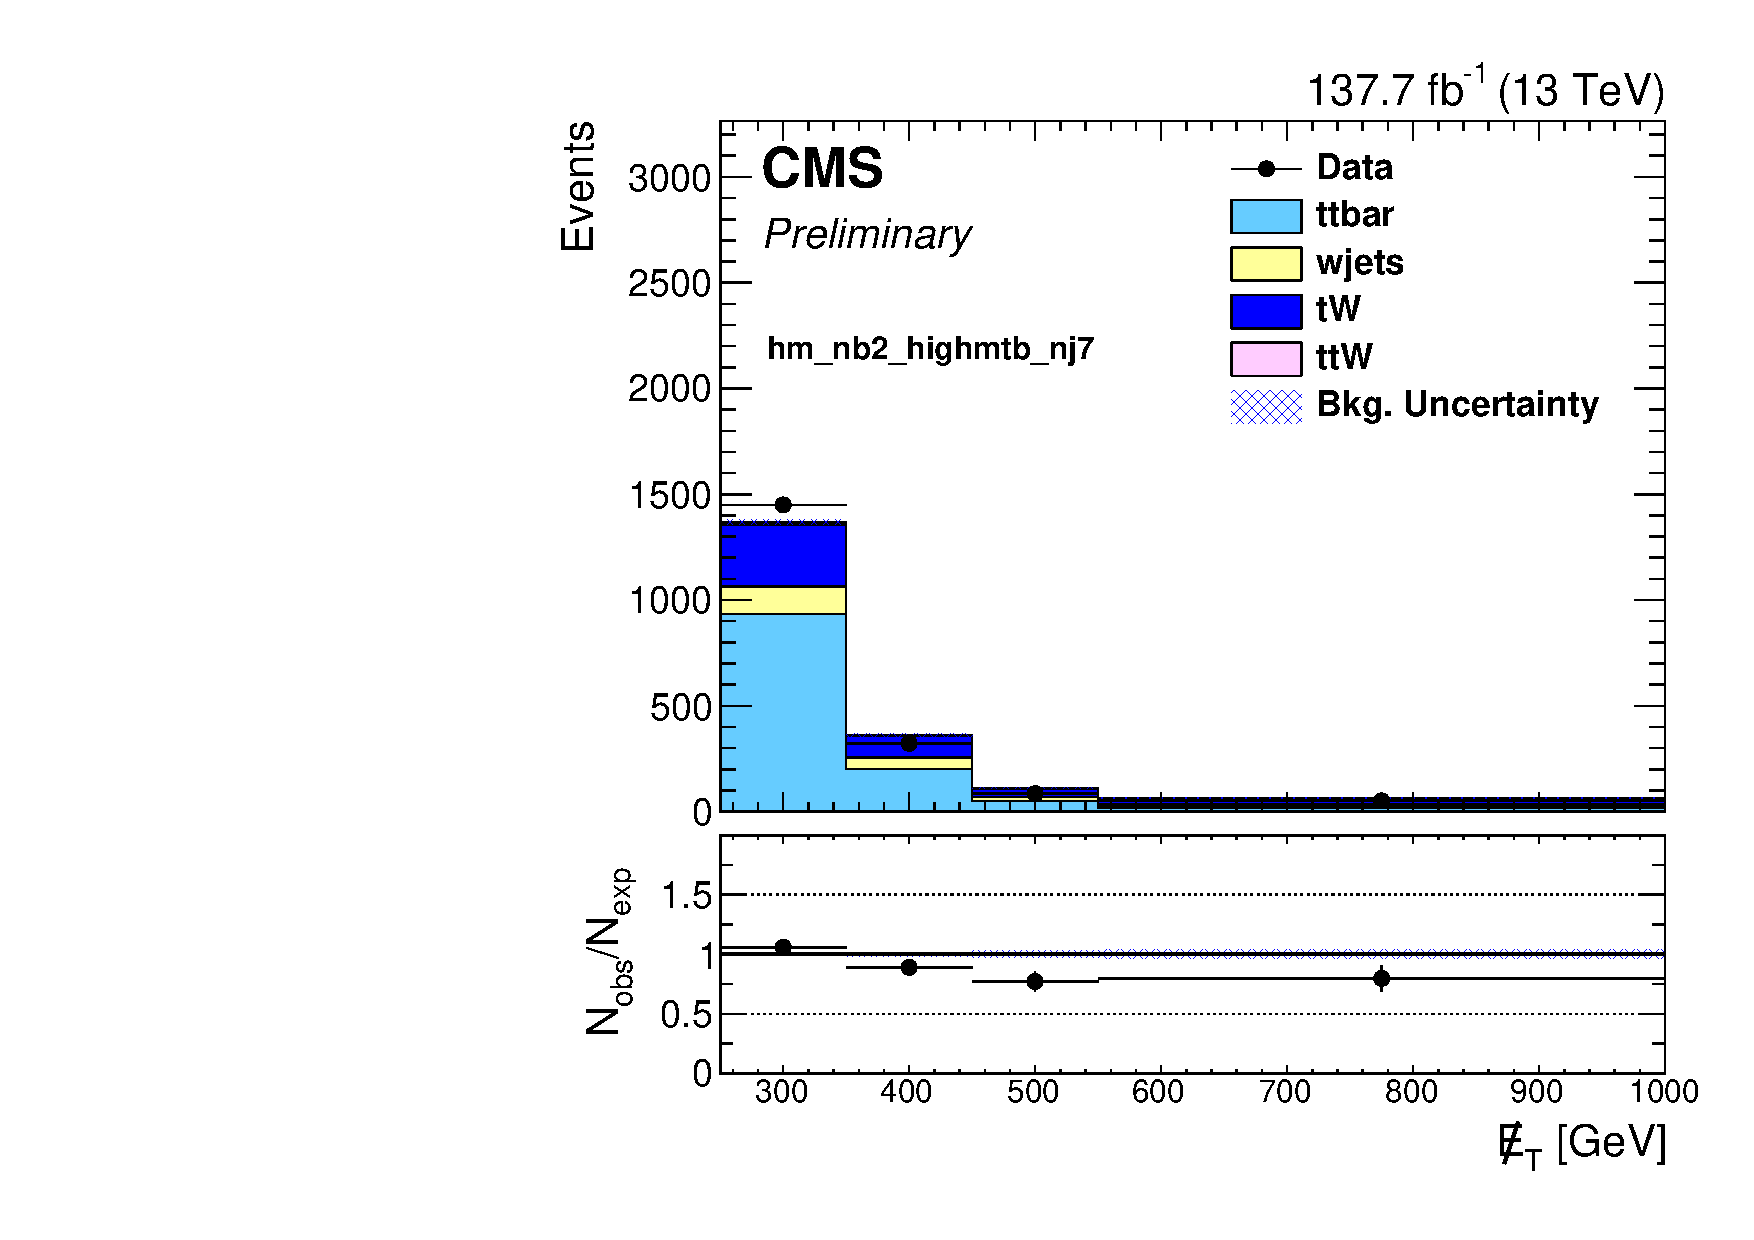
\includegraphics[width=0.32\textwidth]{../Research/SUSY/2019/LLB/lepcr_allEras/MET_pt_DataMC_hm_nb2_highmtb_nj7_nt0_nrt0_nw0__.pdf} \\
	\end{center}
	\caption{Comparison of the \met~distribution in the single-lepton sample after applying the high \dm~baseline selection in the $\mtb<175~\GeV$ and $\nt=0, \nrt=0,$ and $\nw=0$ region. Data and simulation are represented by the black points and stacked histograms, respectively. The error bars on the ratio of observed data to simulation correspond to the data statistical uncertainty and the shaded blue band represents the statistical uncertainty on the simulation. These regions are included with the search regions in the simultaneous fit for the signal extraction in order to estimate the LL contribution.
	 %               The plots in the top row are for events with $\mtb<175$~\GeV, with $5\leq\nj<7$ on the left and $\nj\geq7$ on the right. 
	 %               The plots in the middle row are for events with $\mtb>175$~\GeV and $\nt=0, \nw=0$, with $5\leq\nj<7$ on the left and $\nj\geq7$ on the right. 
	 %               The plot in the bottom row is for events with $\mtb>175$~\GeV and $\nj\geq5$, with $\nt=0, \nw\geq1$ on the left, $\nt\geq1, \nw=0$ on the middle, and $\nt\geq1$, and $\nw\geq1$ on the right.
	 }
	\label{fig:llb-1lcr-datavsmc-hm-nt0-nrt0-nw0}
\end{figure}

\begin{figure}[!htb]
	\begin{center}
  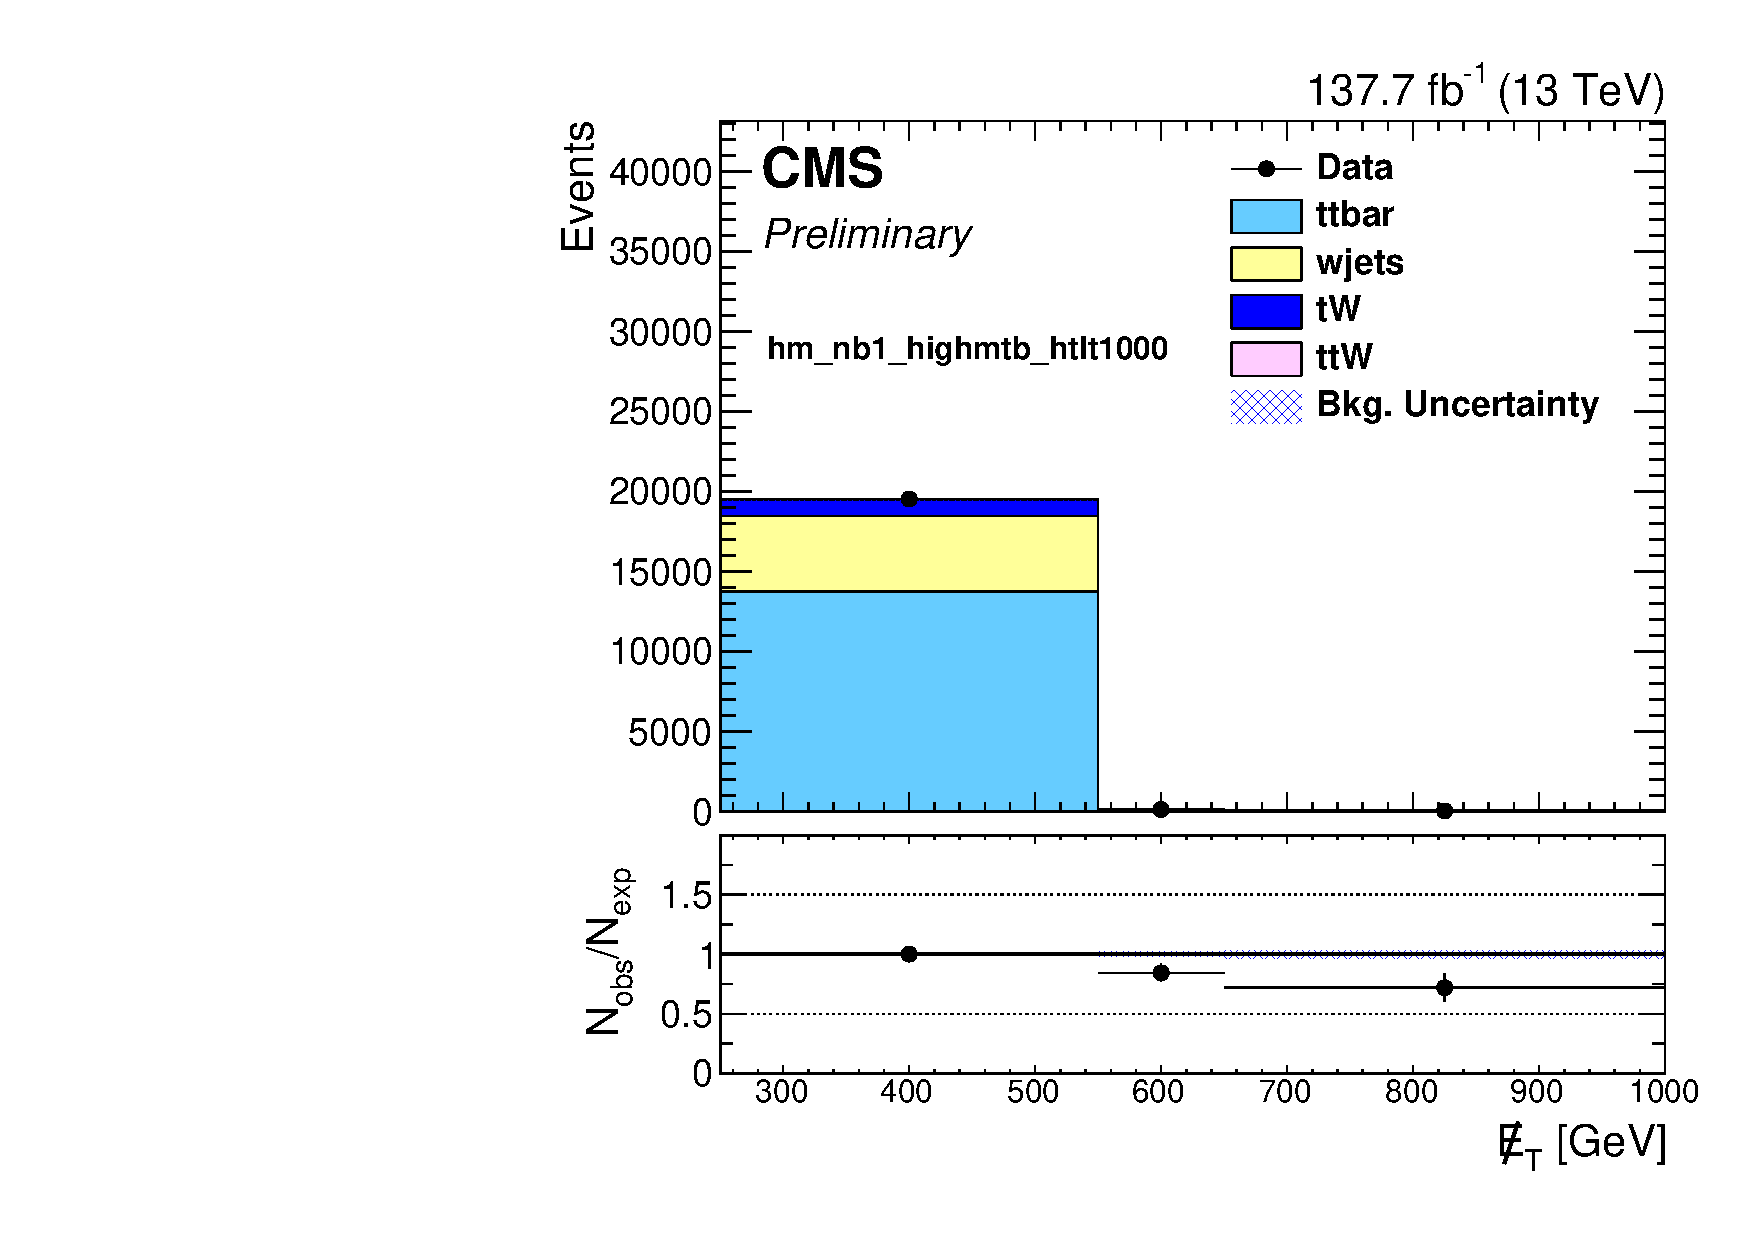
\includegraphics[width=0.32\textwidth]{../Research/SUSY/2019/LLB/lepcr_allEras/MET_pt_DataMC_hm_nb1_highmtb_ntgeq1_nrt0_nw0_htlt1000__.pdf}
  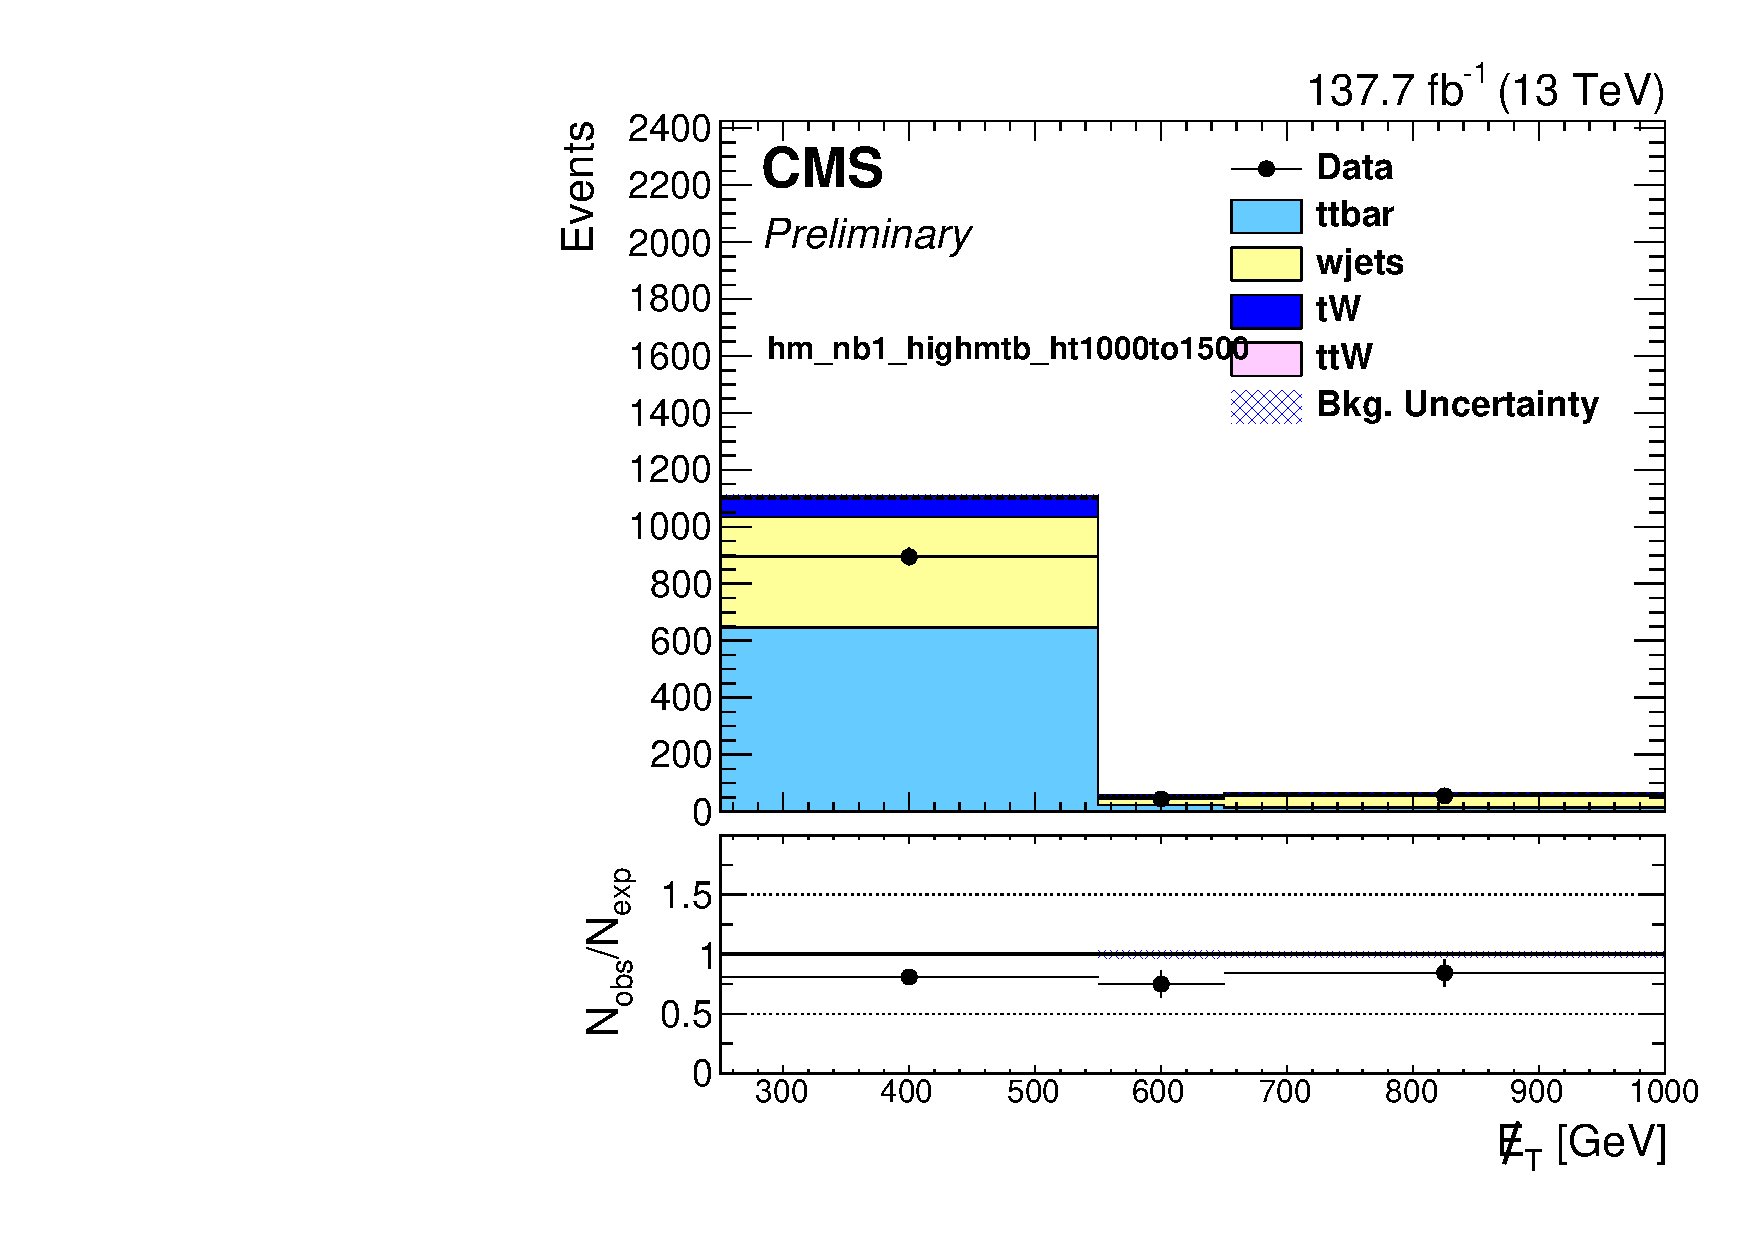
\includegraphics[width=0.32\textwidth]{../Research/SUSY/2019/LLB/lepcr_allEras/MET_pt_DataMC_hm_nb1_highmtb_ntgeq1_nrt0_nw0_ht1000to1500__.pdf}
  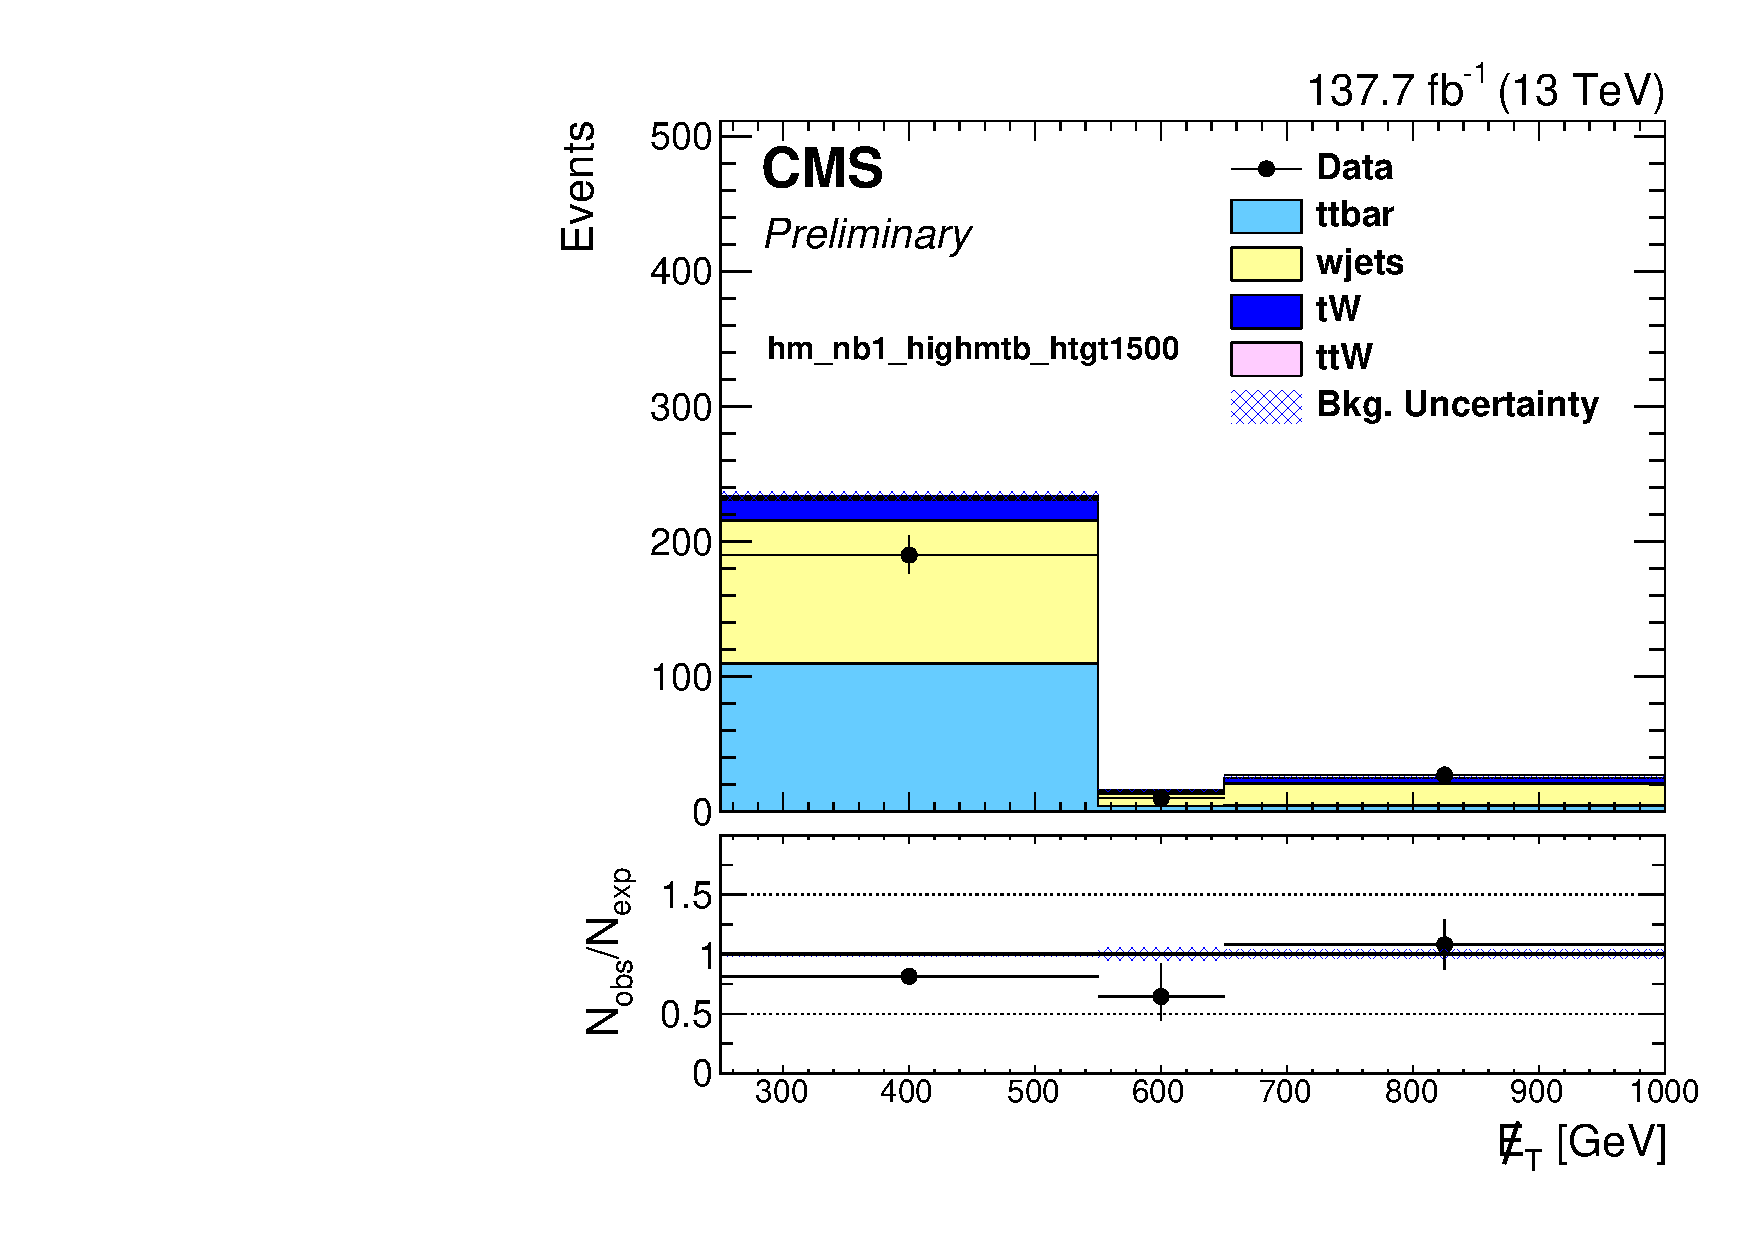
\includegraphics[width=0.32\textwidth]{../Research/SUSY/2019/LLB/lepcr_allEras/MET_pt_DataMC_hm_nb1_highmtb_ntgeq1_nrt0_nw0_htgt1500__.pdf} \\
  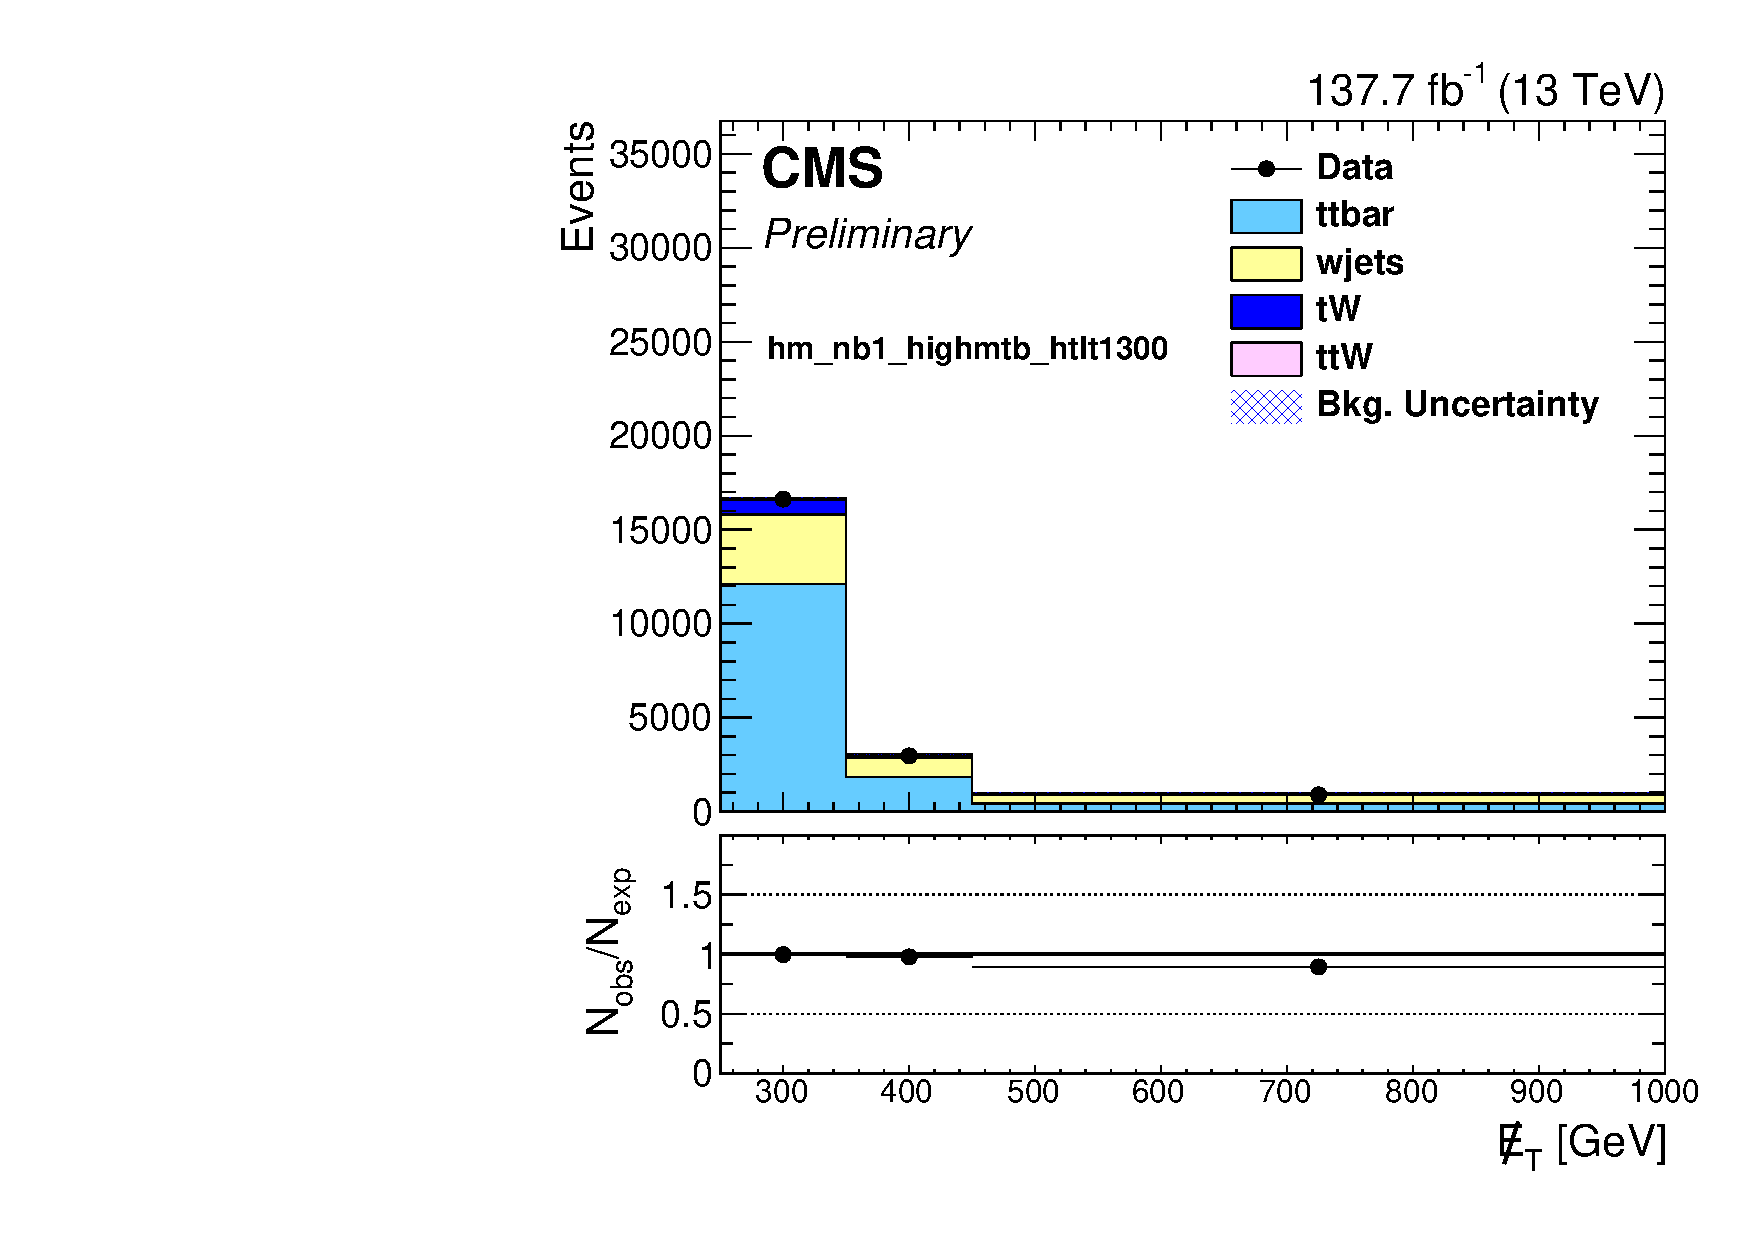
\includegraphics[width=0.32\textwidth]{../Research/SUSY/2019/LLB/lepcr_allEras/MET_pt_DataMC_hm_nb1_highmtb_nt0_nrt0_nwgeq1_htlt1300__.pdf} 
  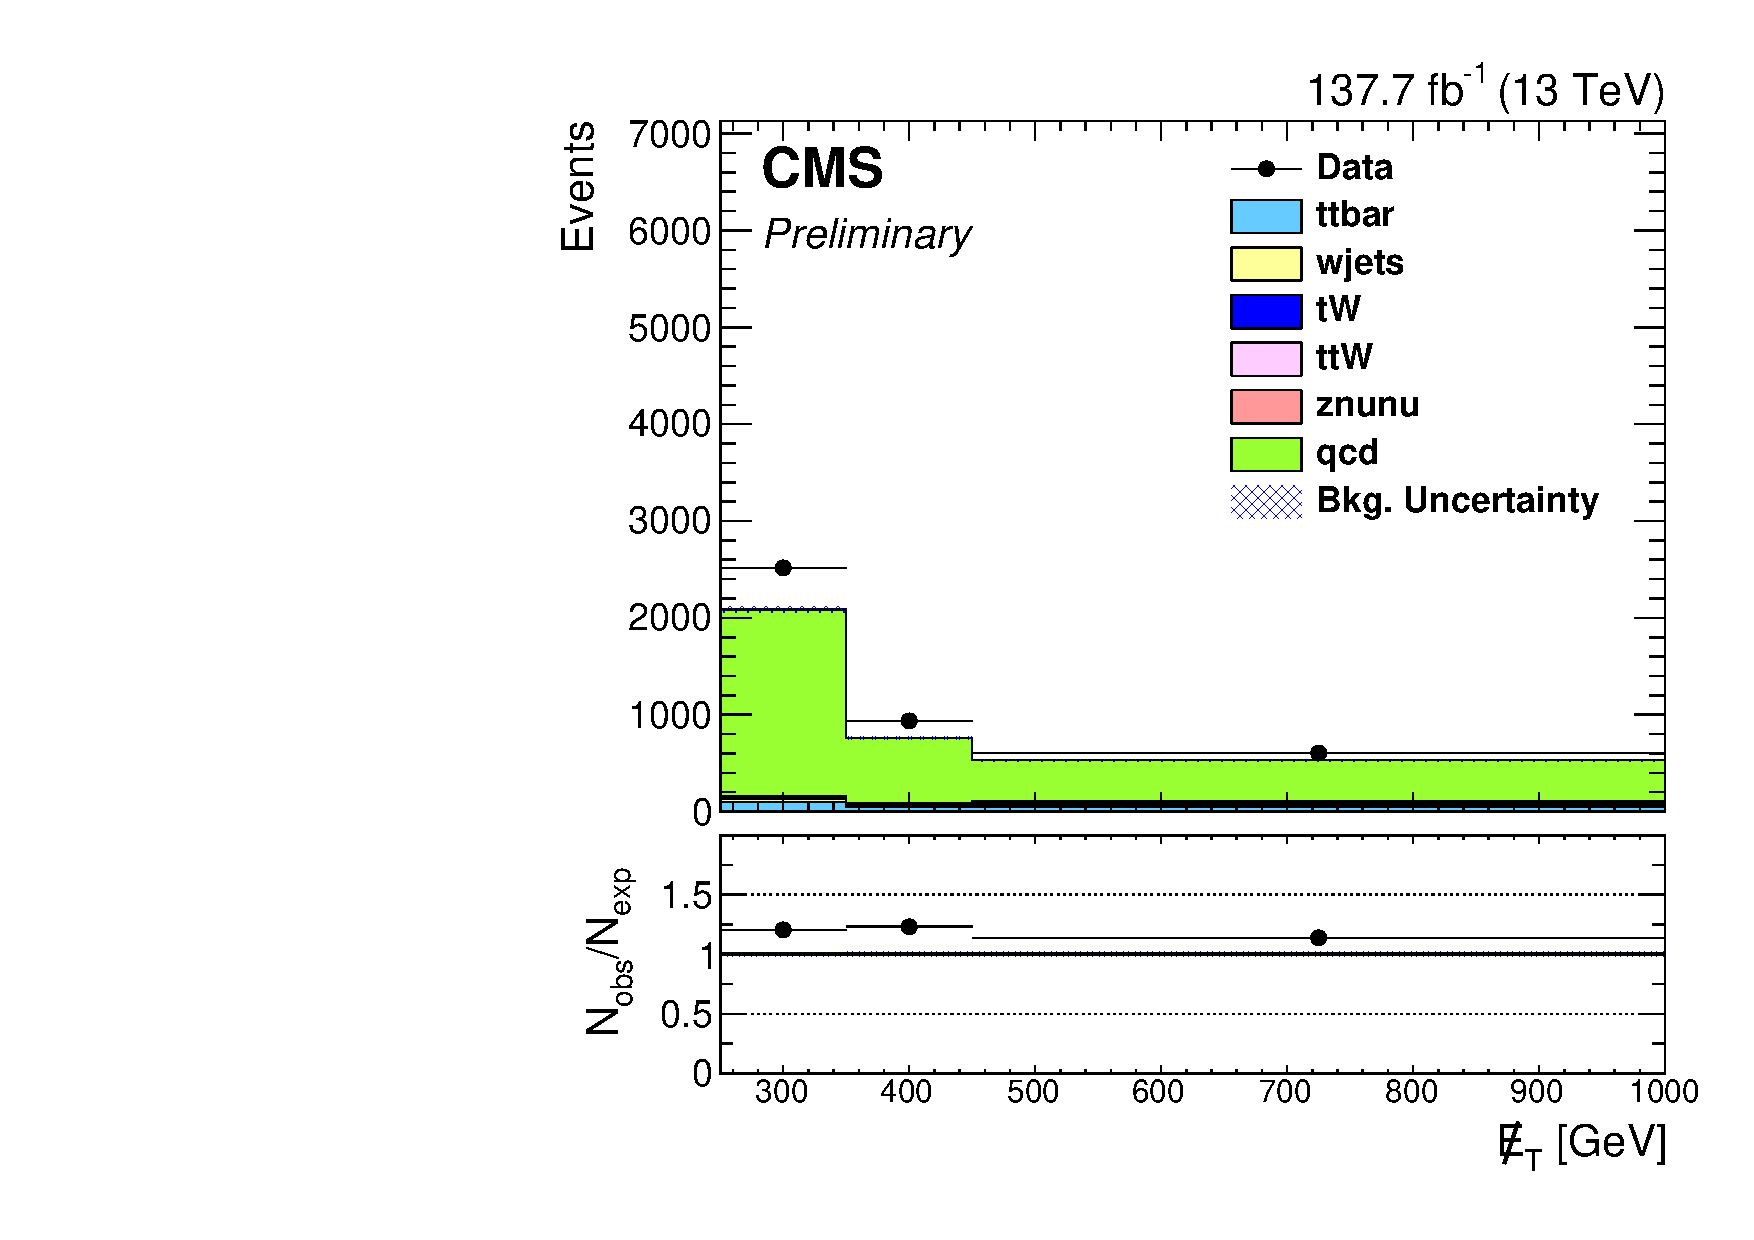
\includegraphics[width=0.32\textwidth]{../Research/SUSY/2019/LLB/lepcr_allEras/MET_pt_DataMC_hm_nb1_highmtb_nt0_nrt0_nwgeq1_htgt1300__.pdf} \\
  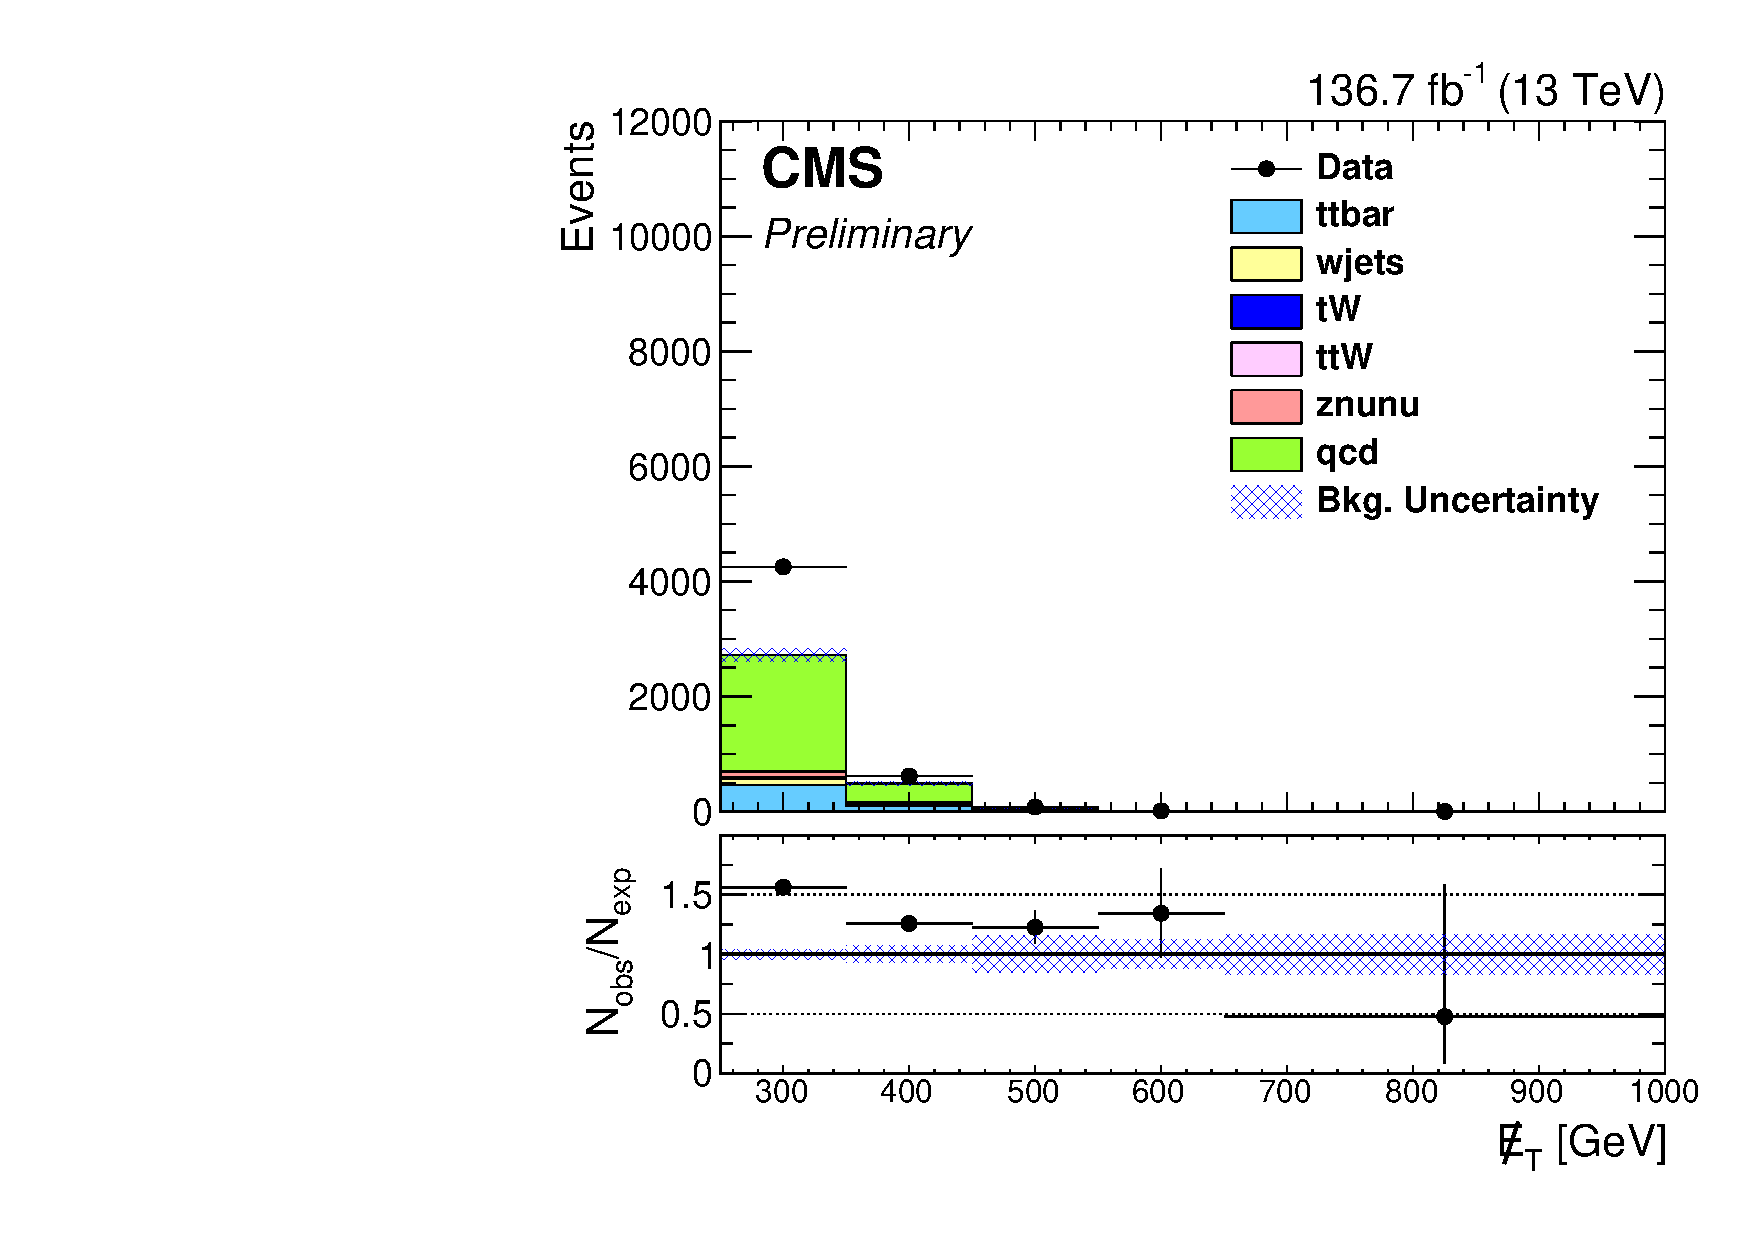
\includegraphics[width=0.32\textwidth]{../Research/SUSY/2019/LLB/lepcr_allEras/MET_pt_DataMC_hm_nb1_highmtb_nt0_nrtgeq1_nw0_htlt1000__.pdf} 
  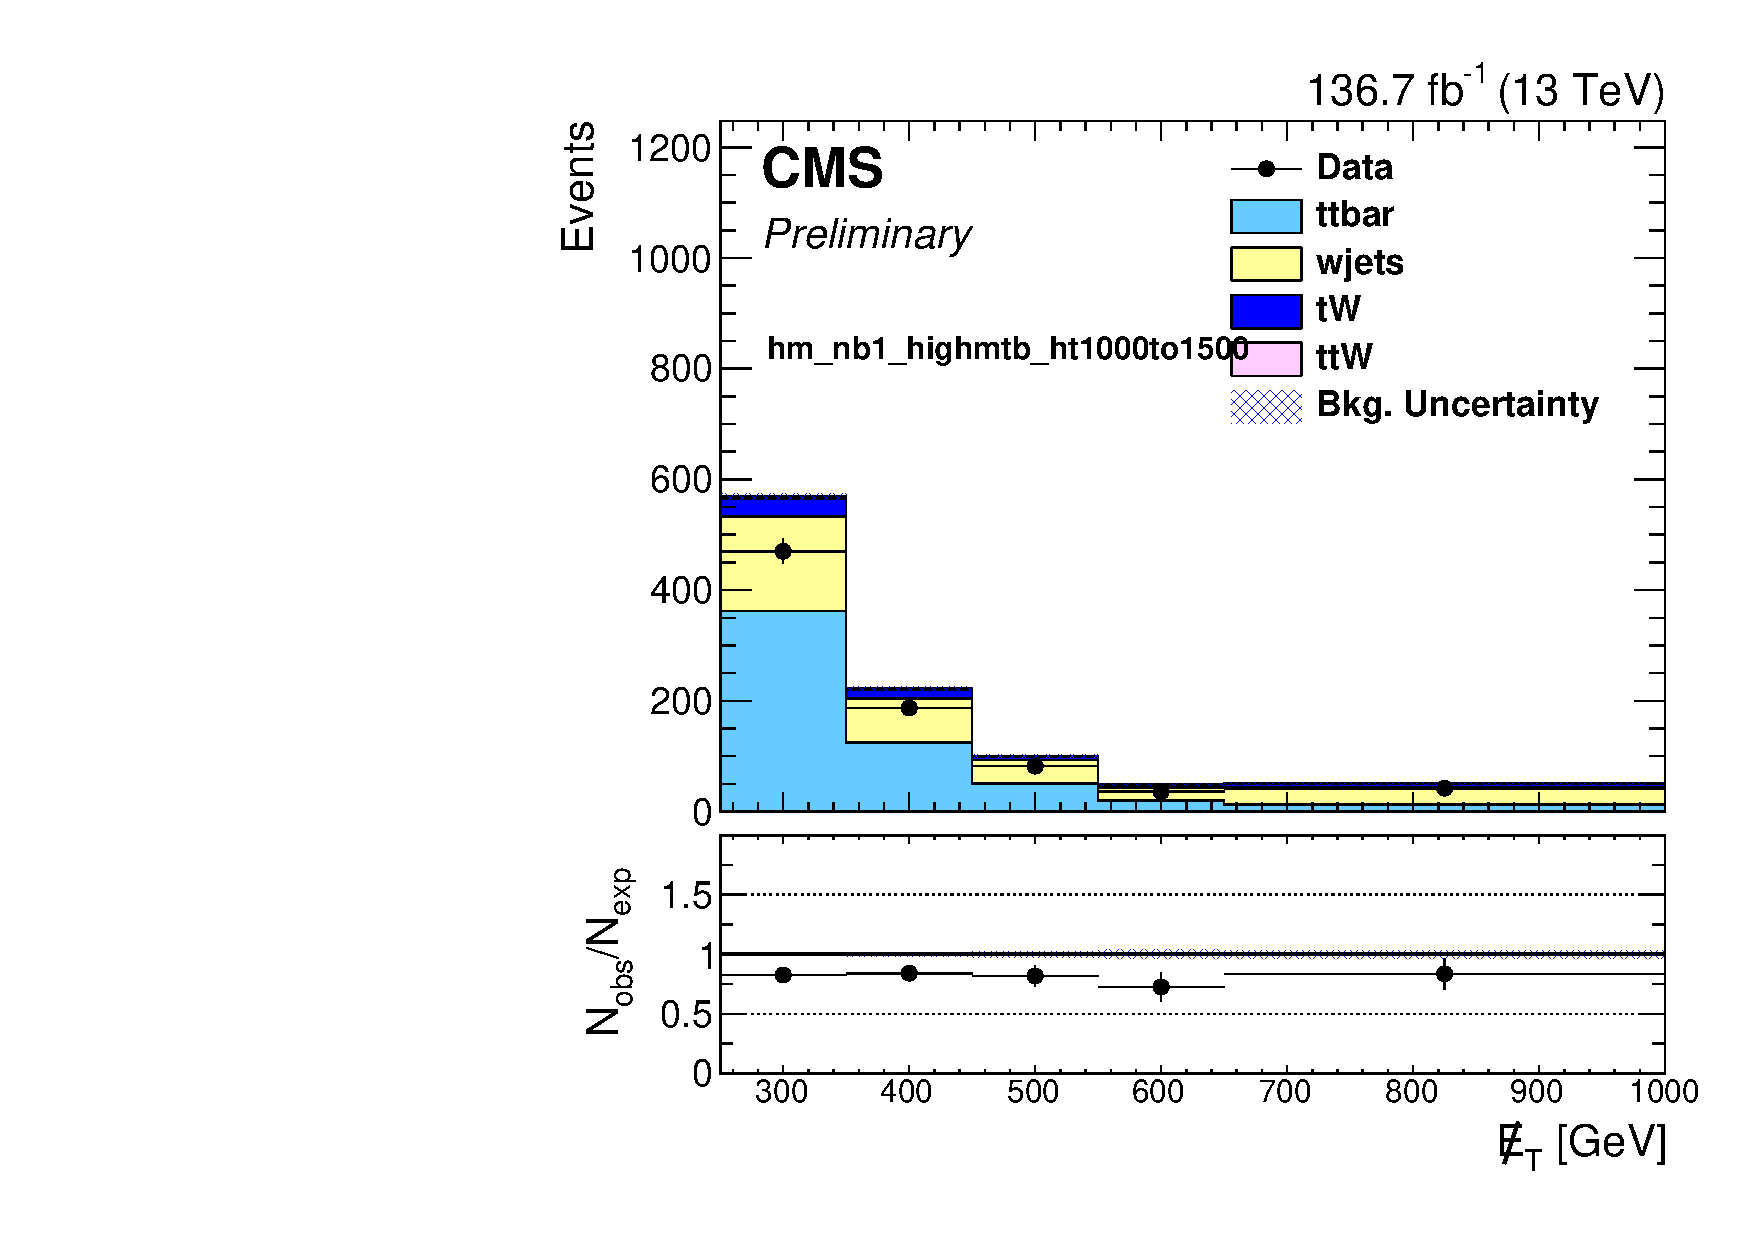
\includegraphics[width=0.32\textwidth]{../Research/SUSY/2019/LLB/lepcr_allEras/MET_pt_DataMC_hm_nb1_highmtb_nt0_nrtgeq1_nw0_ht1000to1500__.pdf} 
  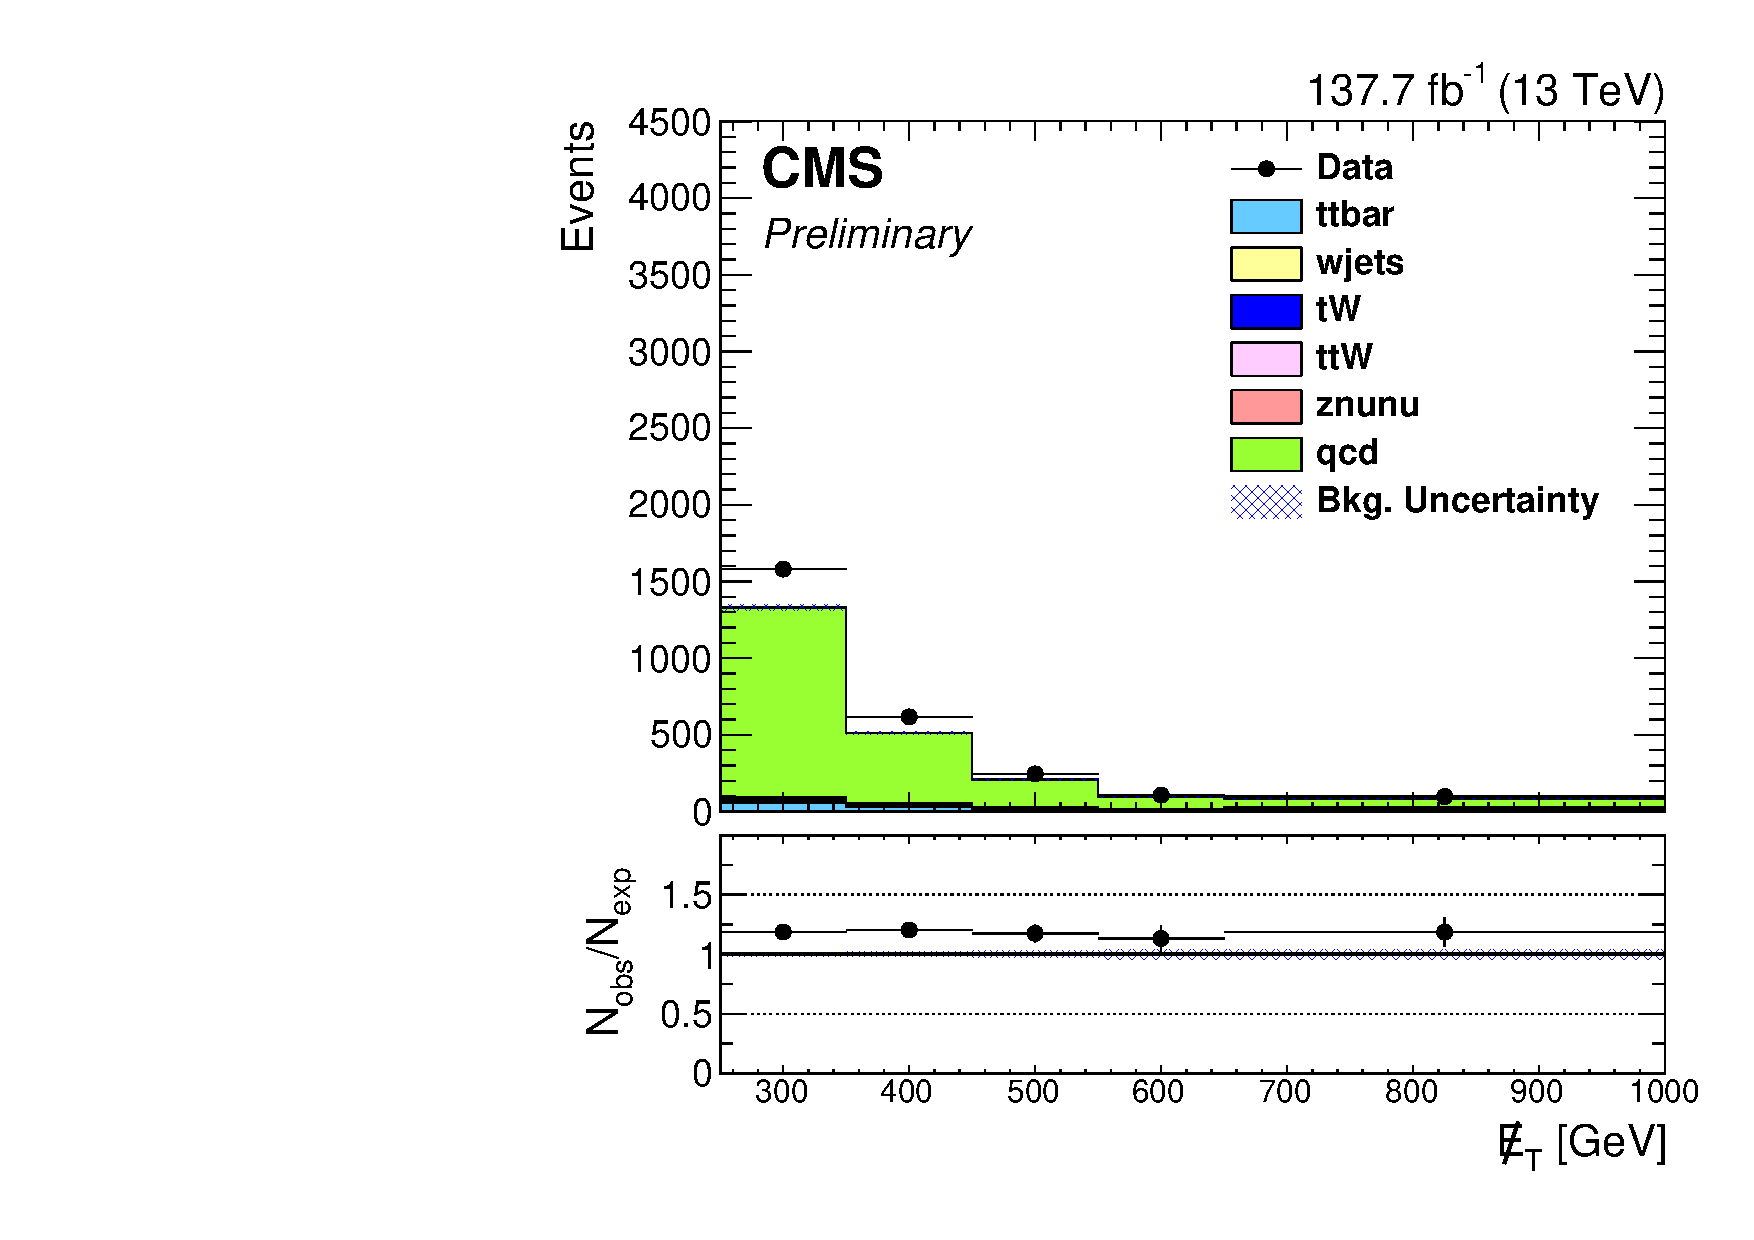
\includegraphics[width=0.32\textwidth]{../Research/SUSY/2019/LLB/lepcr_allEras/MET_pt_DataMC_hm_nb1_highmtb_nt0_nrtgeq1_nw0_htgt1500__.pdf} \\
  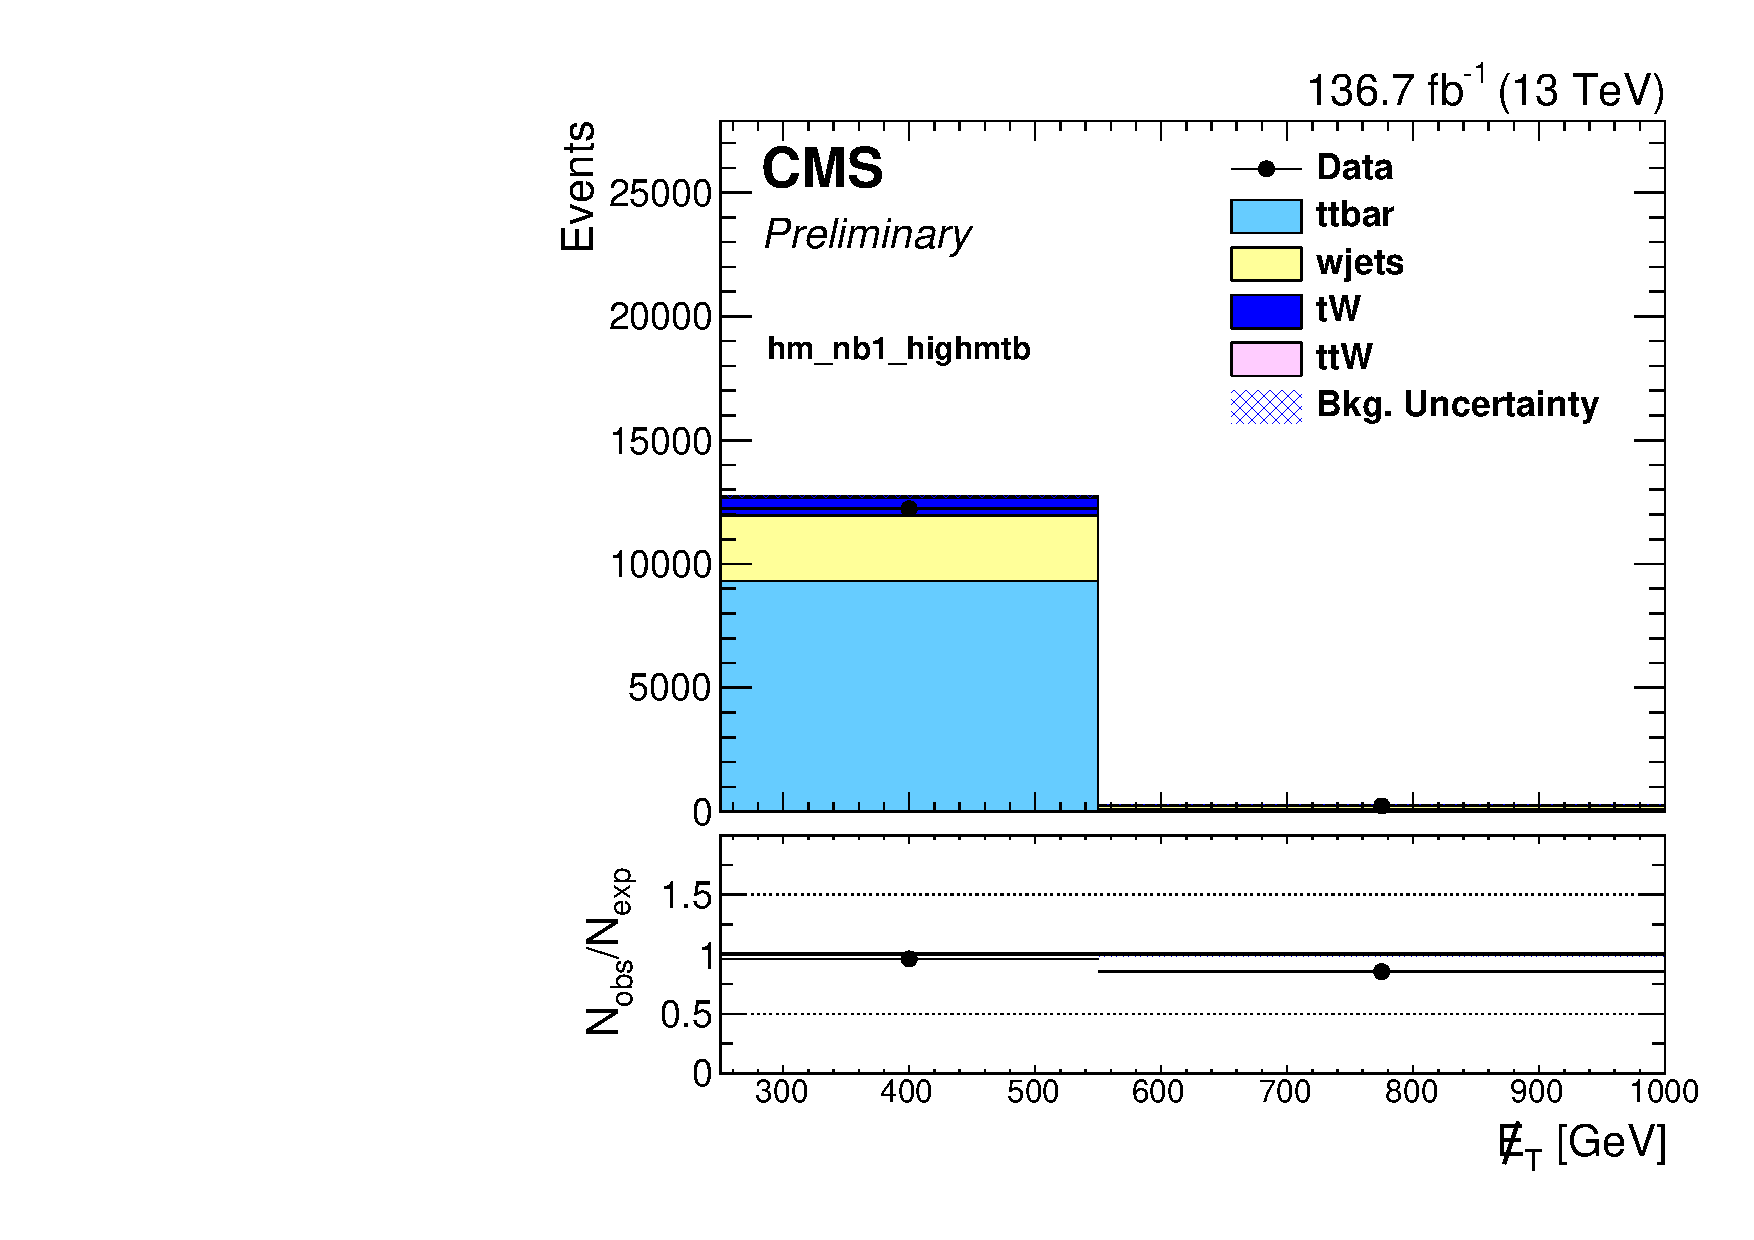
\includegraphics[width=0.32\textwidth]{../Research/SUSY/2019/LLB/lepcr_allEras/MET_pt_DataMC_hm_nb1_highmtb_ntgeq1_nrt0_nwgeq1__.pdf} 
  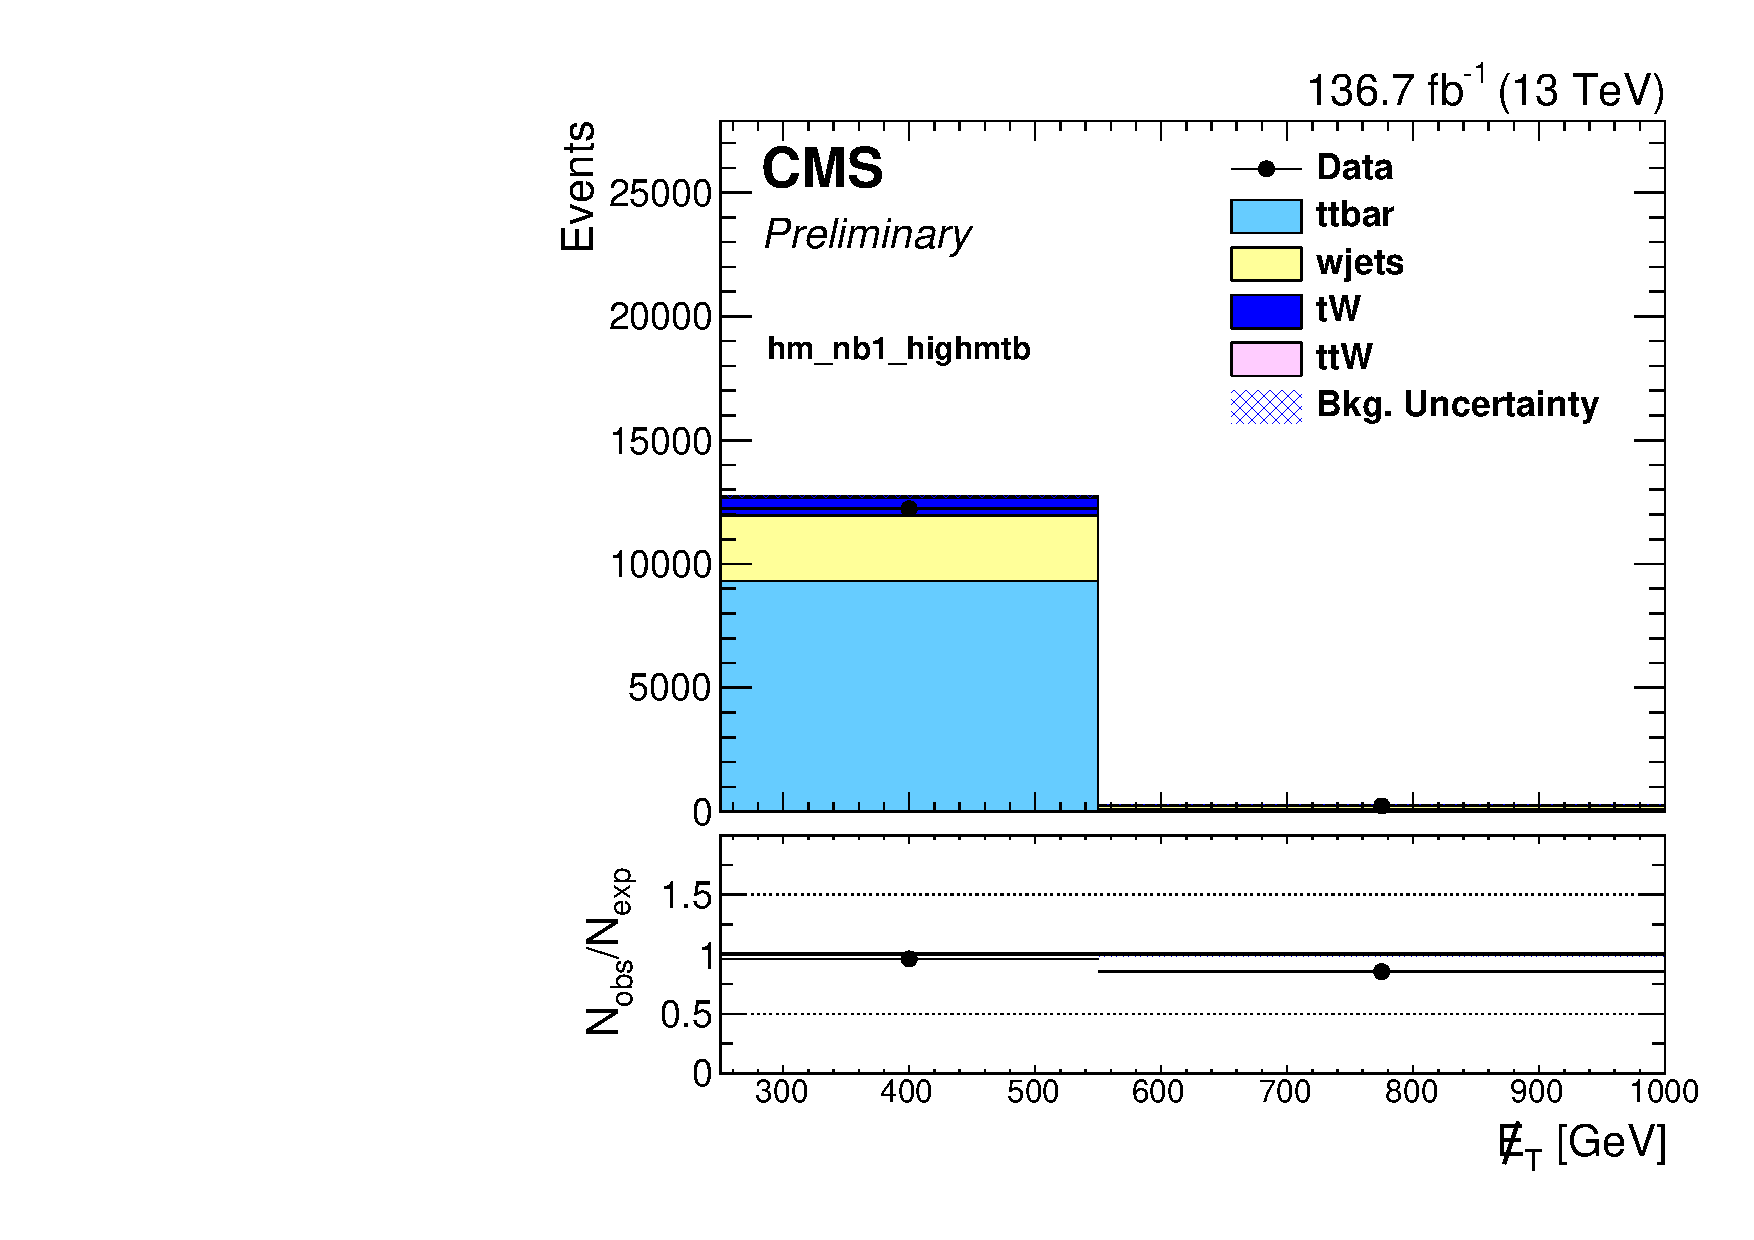
\includegraphics[width=0.32\textwidth]{../Research/SUSY/2019/LLB/lepcr_allEras/MET_pt_DataMC_hm_nb1_highmtb_ntgeq1_nrtgeq1_nw0__.pdf} 
  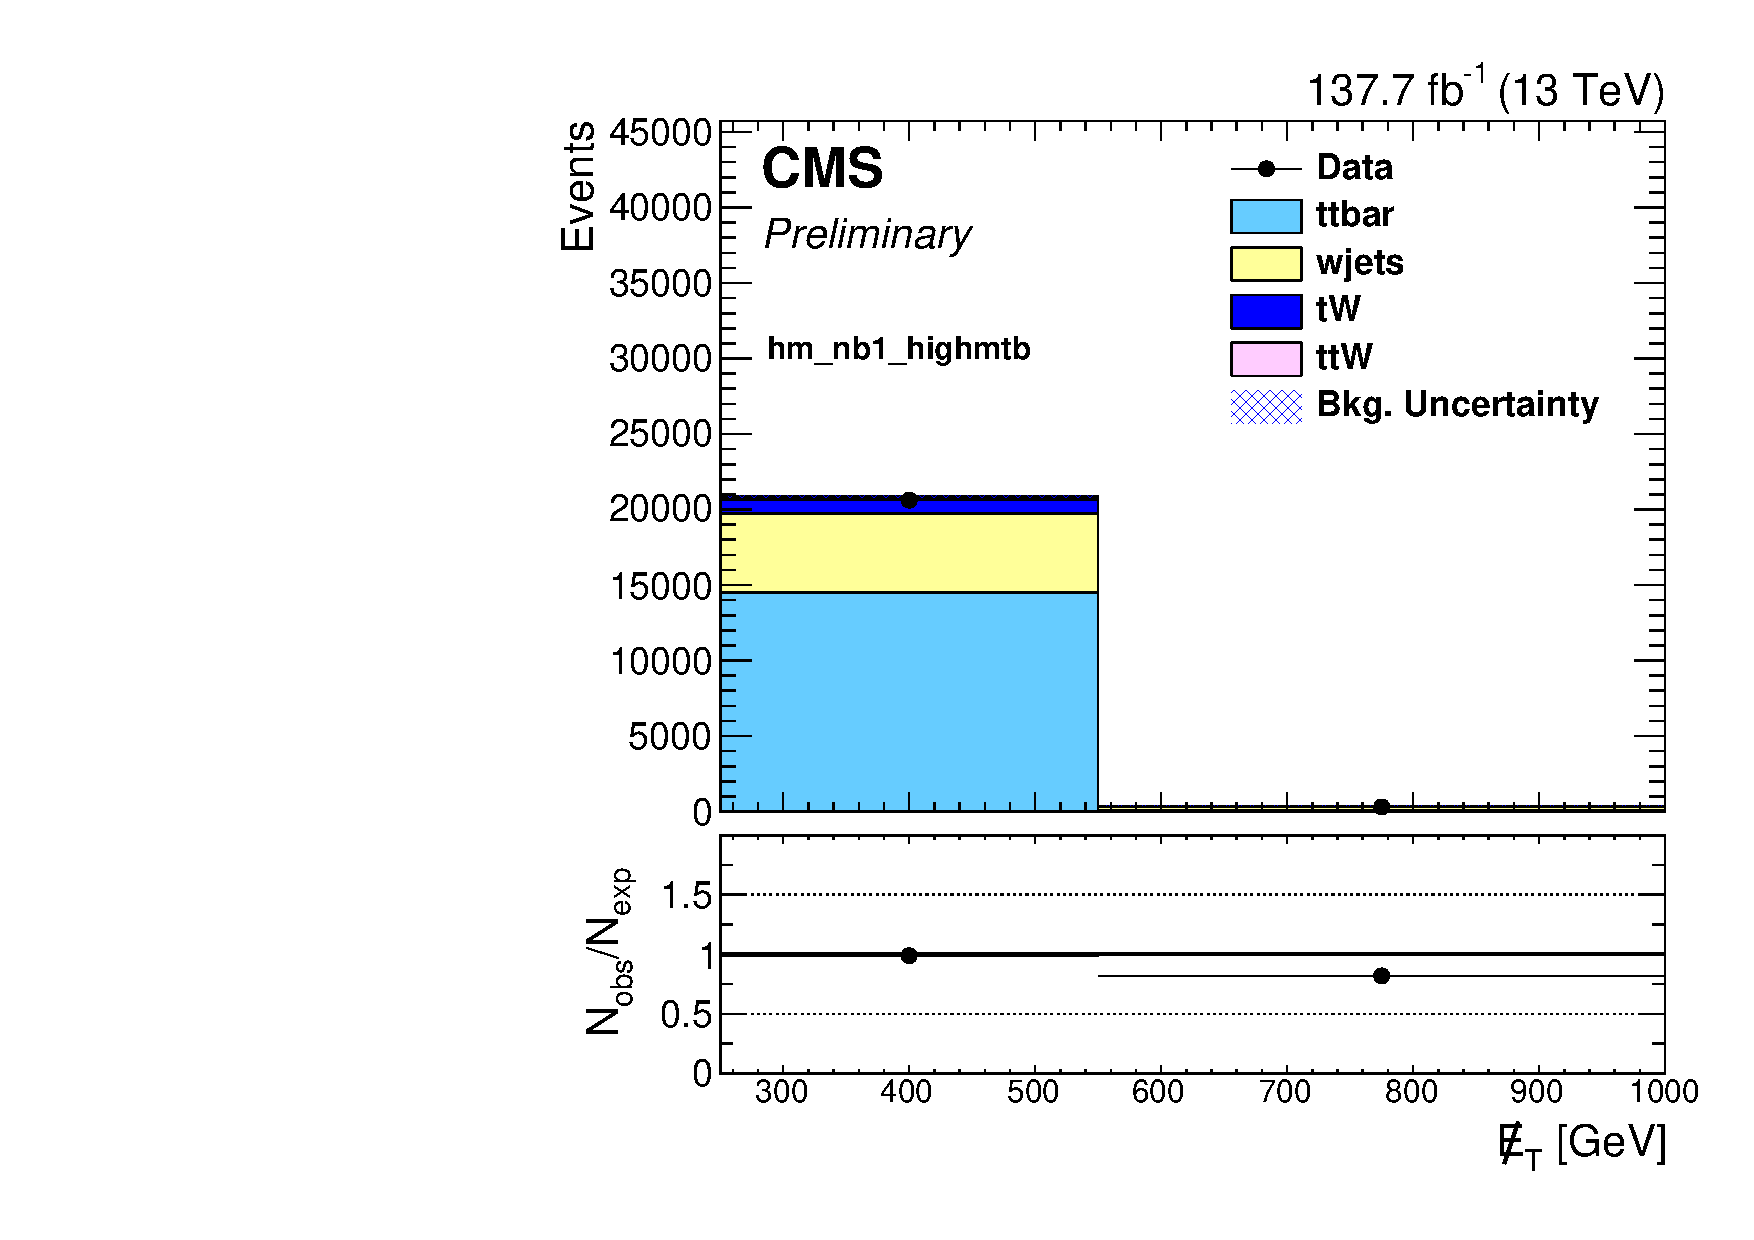
\includegraphics[width=0.32\textwidth]{../Research/SUSY/2019/LLB/lepcr_allEras/MET_pt_DataMC_hm_nb1_highmtb_nt0_nrtgeq1_nwgeq1__.pdf} \\
	\end{center}
	\caption{Comparison of the \met~distribution in the single-lepton sample after applying the high \dm~baseline selection in the $\nb=1$ region where there are $\geq1$ heavy object tags. Data and simulation are represented by the black points and stacked histograms, respectively. The error bars on the ratio of observed data to simulation correspo    nd to the data statistical uncertainty and the shaded blue band represents the statistical uncertainty on the simulation. These regions are included with the search regions in the simultaneous fit for the signal extraction in order to estimate the LL contribution.
	 %               The plots in the top row are for events with $\mtb<175$~\GeV, with $5\leq\nj<7$ on the left and $\nj\geq7$ on the right. 
	 %               The plots in the middle row are for events with $\mtb>175$~\GeV and $\nt=0, \nw=0$, with $5\leq\nj<7$ on the left and $\nj\geq7$ on the right. 
	 %               The plot in the bottom row is for events with $\mtb>175$~\GeV and $\nj\geq5$, with $\nt=0, \nw\geq1$ on the left, $\nt\geq1, \nw=0$ on the middle, and $\nt\geq1$, and $\nw\geq1$ on the right.
	 }
	\label{fig:llb-1lcr-datavsmc-hm-nb1}
\end{figure}

\begin{figure}[!htb]
	\begin{center}
  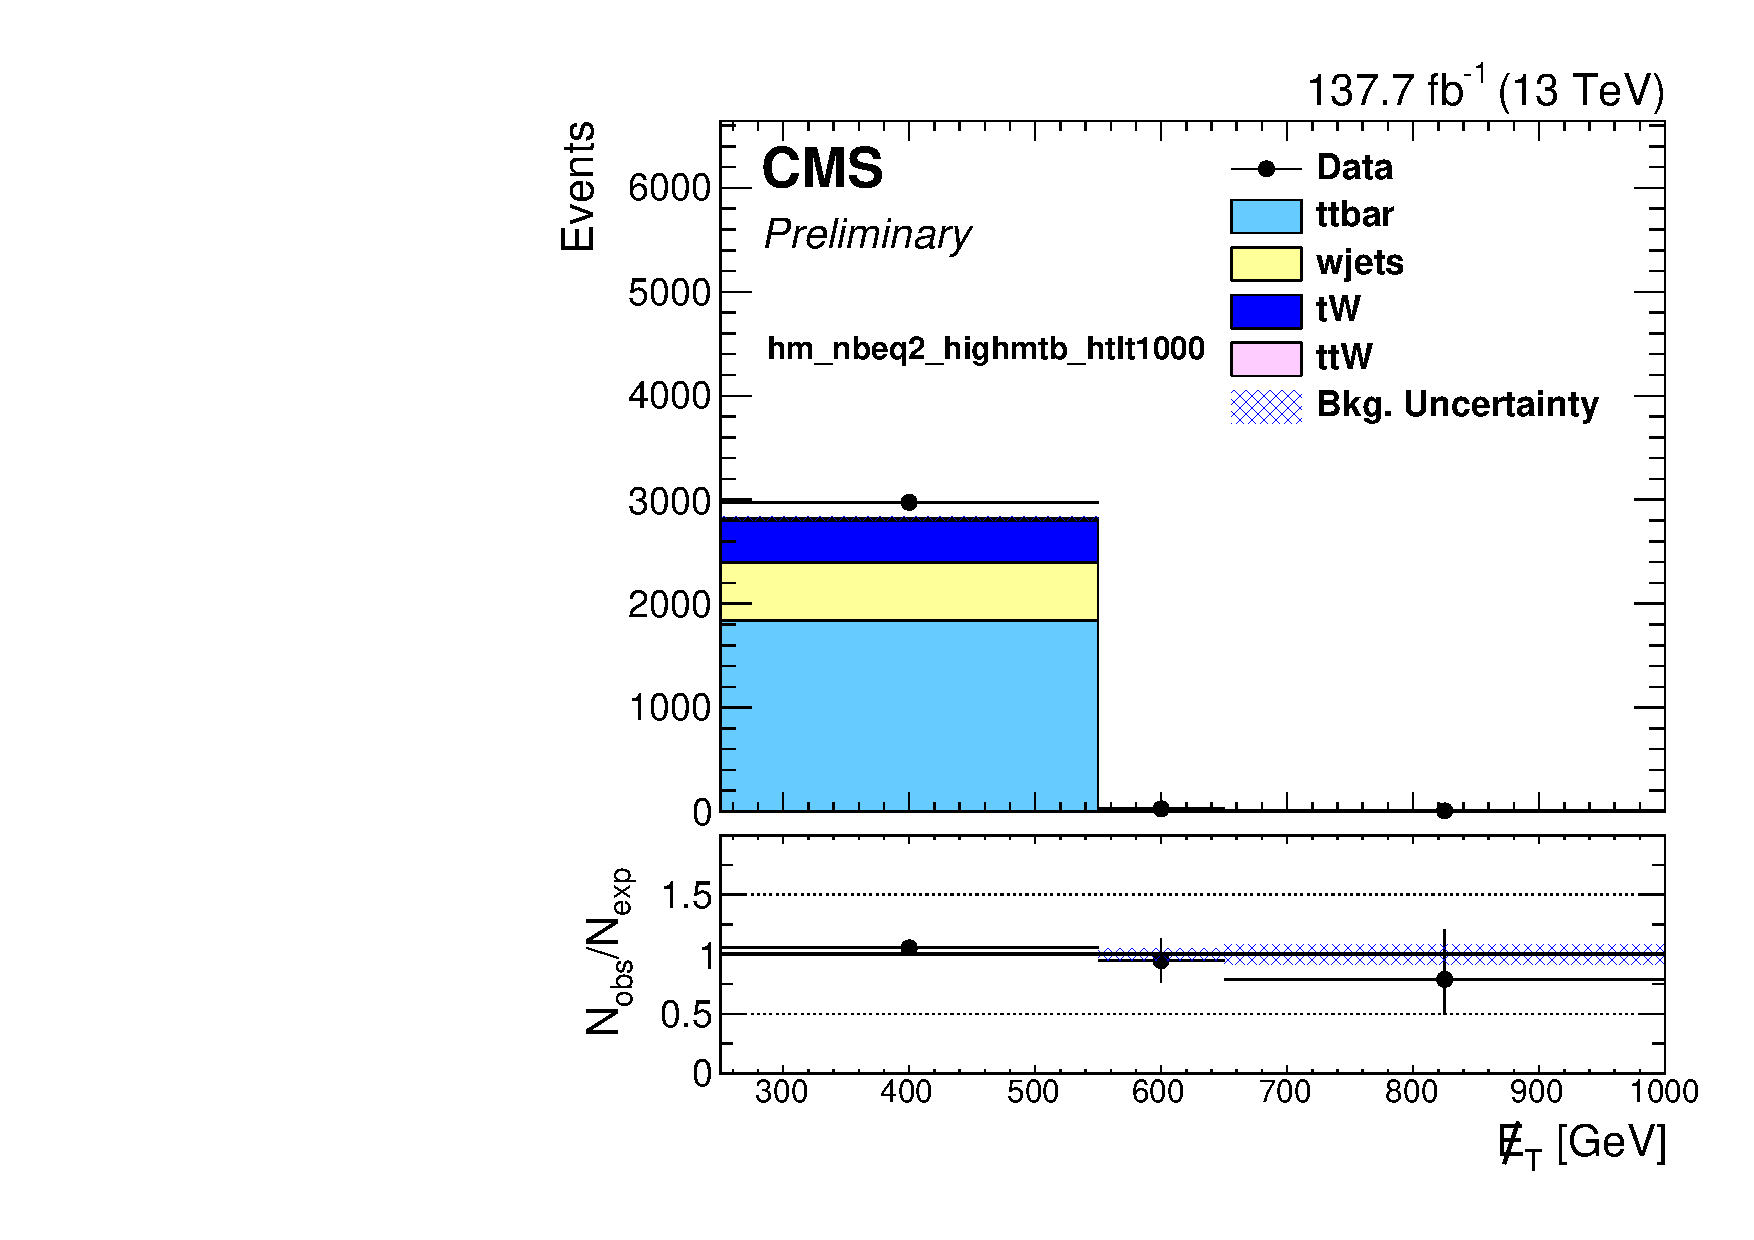
\includegraphics[width=0.32\textwidth]{../Research/SUSY/2019/LLB/lepcr_allEras/MET_pt_DataMC_hm_nbeq2_highmtb_nt1_nrt0_nw0_htlt1000__.pdf}
  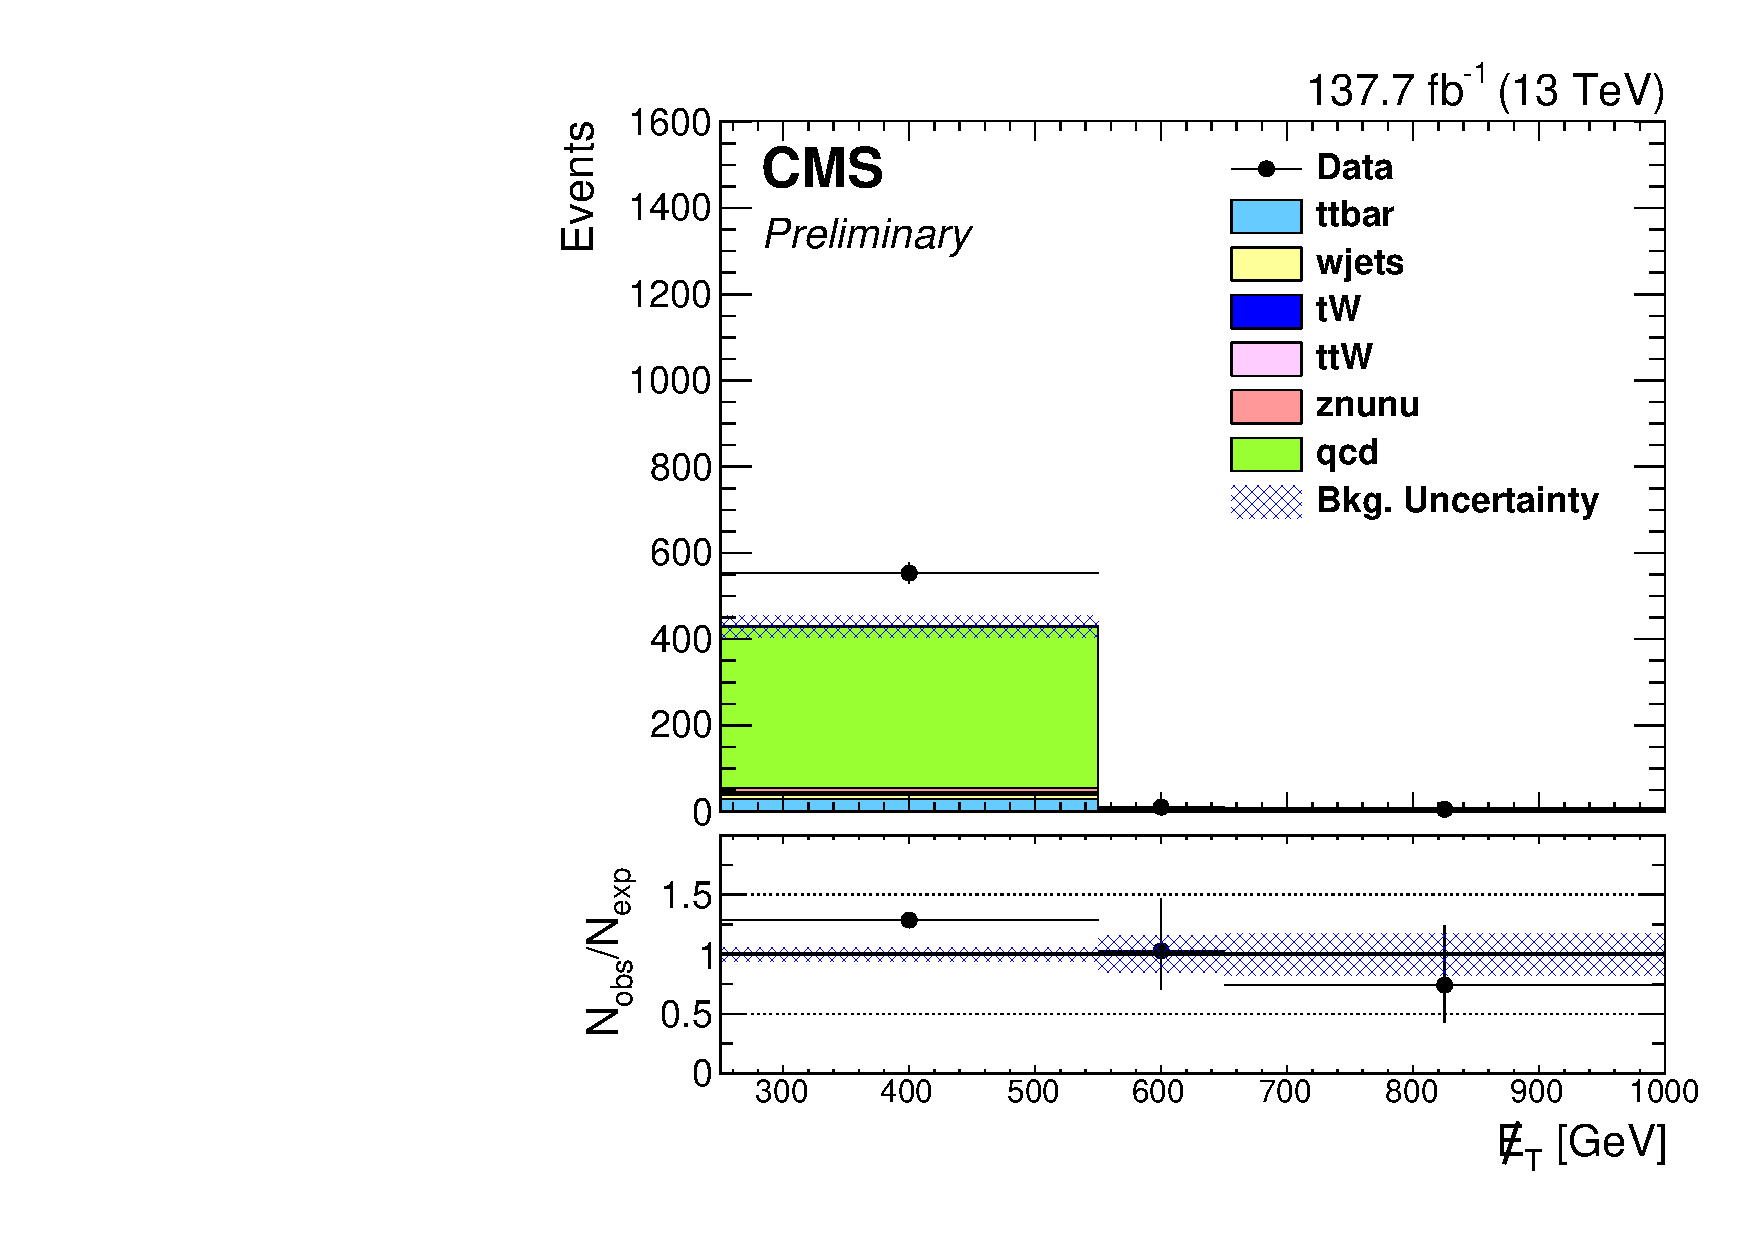
\includegraphics[width=0.32\textwidth]{../Research/SUSY/2019/LLB/lepcr_allEras/MET_pt_DataMC_hm_nbeq2_highmtb_nt1_nrt0_nw0_ht1000to1500__.pdf}
  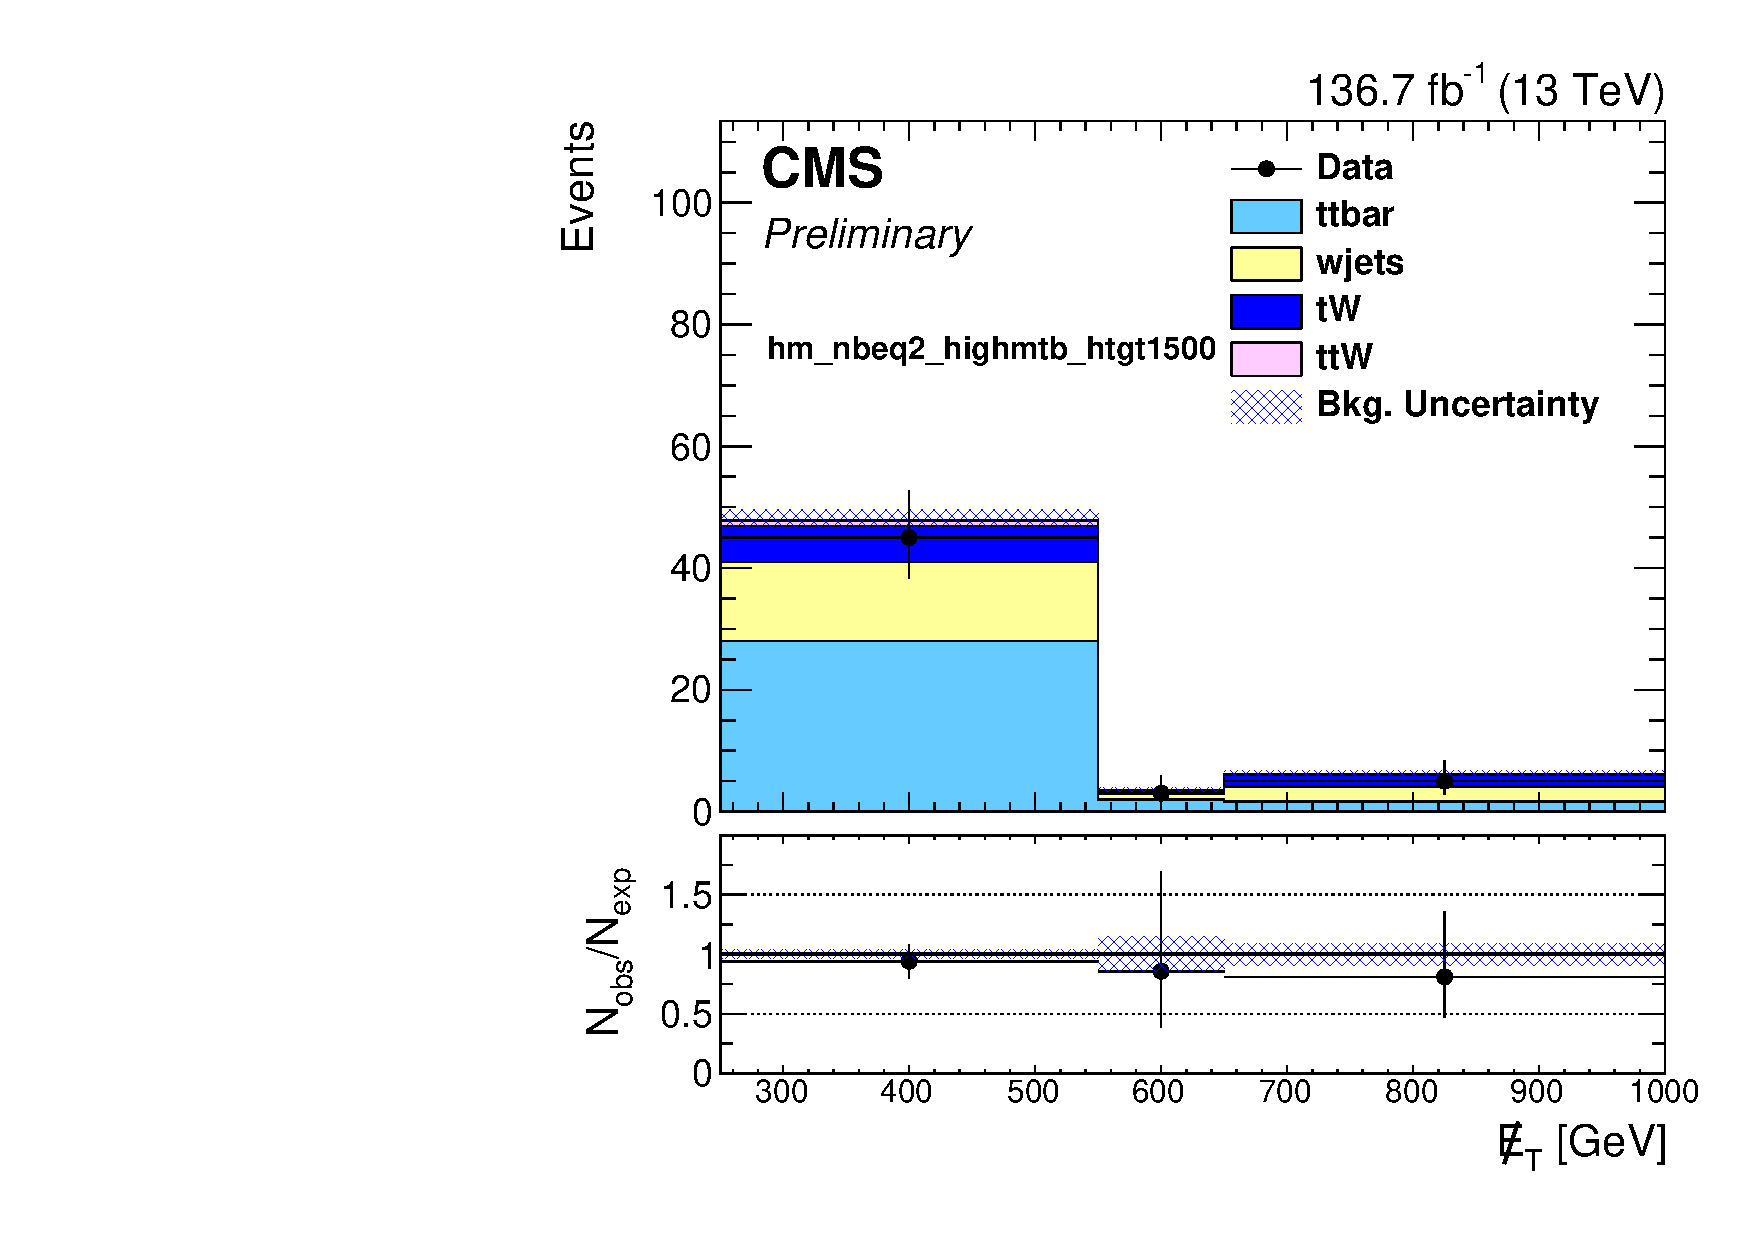
\includegraphics[width=0.32\textwidth]{../Research/SUSY/2019/LLB/lepcr_allEras/MET_pt_DataMC_hm_nbeq2_highmtb_nt1_nrt0_nw0_htgt1500__.pdf} \\
  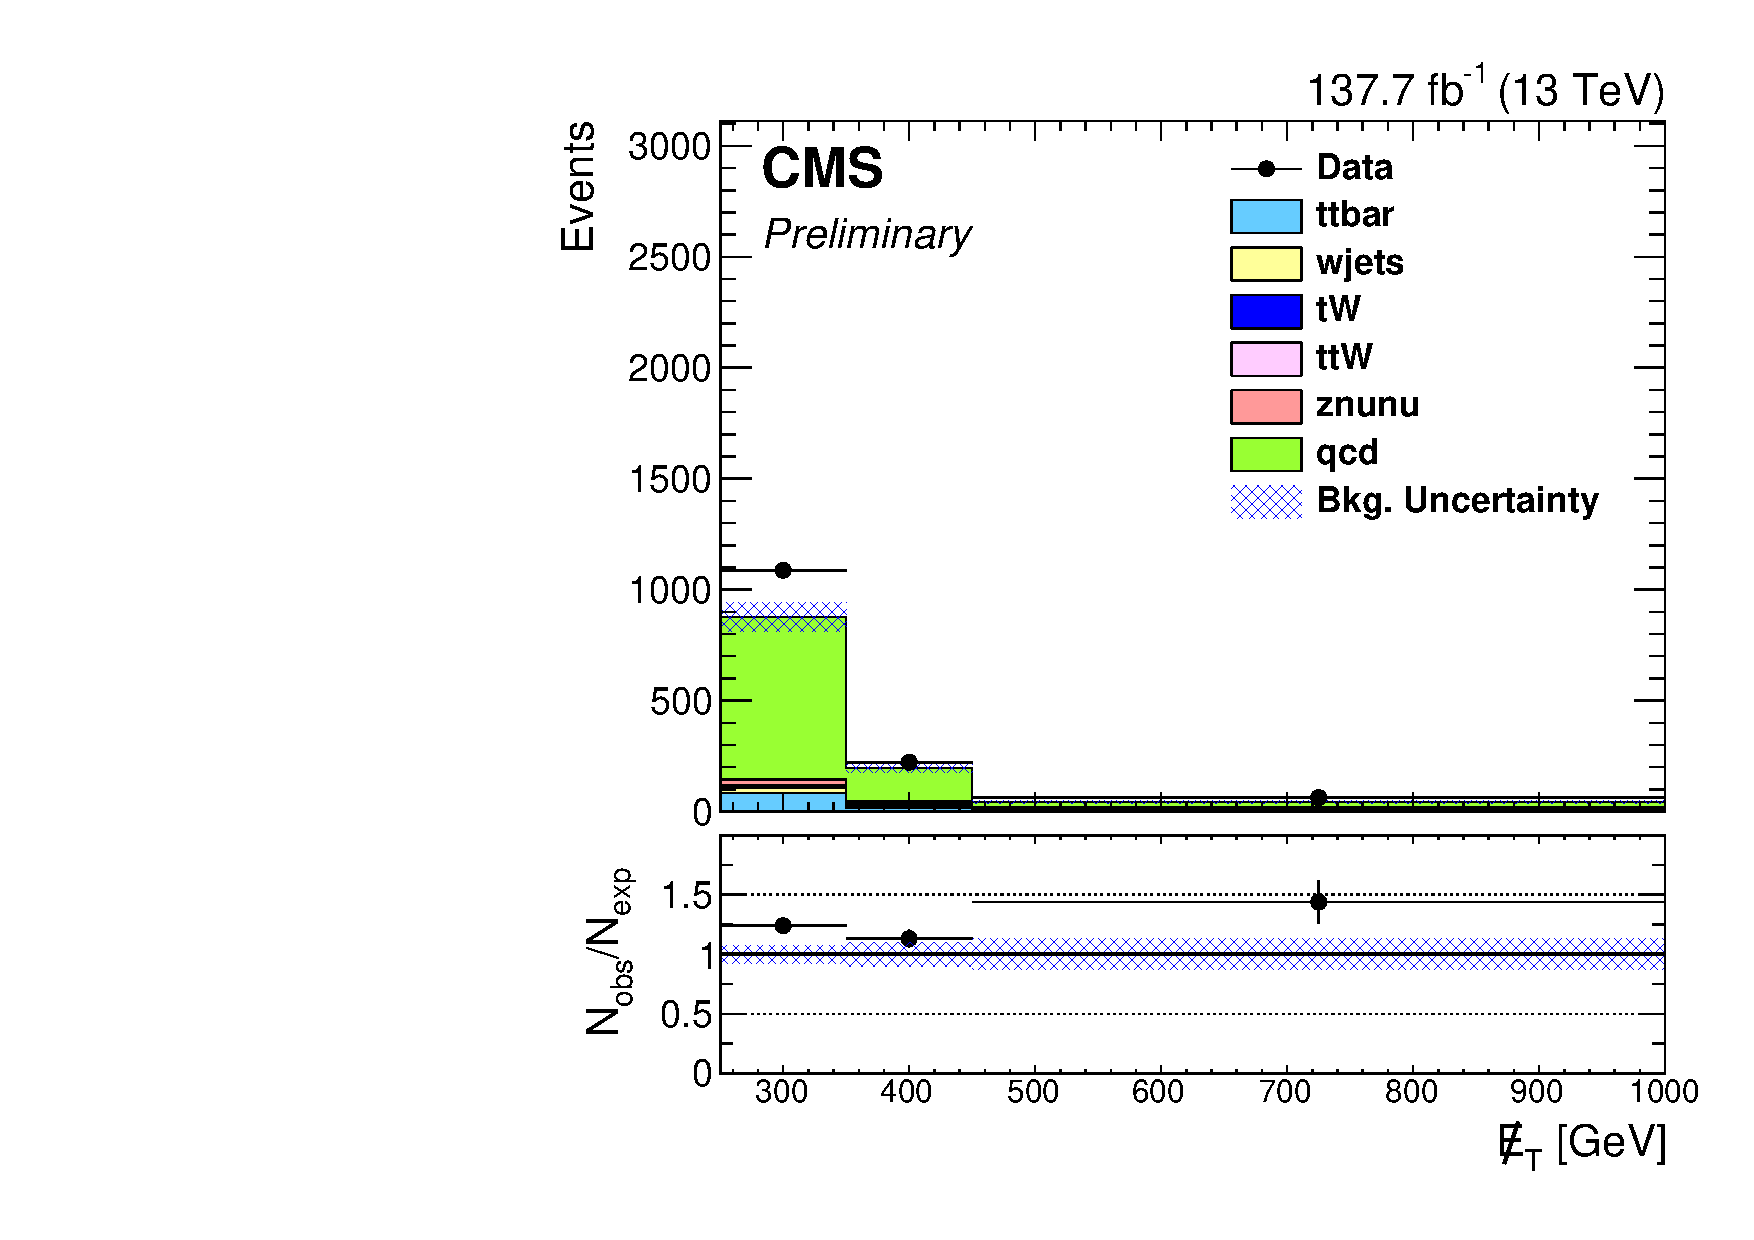
\includegraphics[width=0.32\textwidth]{../Research/SUSY/2019/LLB/lepcr_allEras/MET_pt_DataMC_hm_nbeq2_highmtb_nt0_nrt0_nw1_htlt1300__.pdf} 
  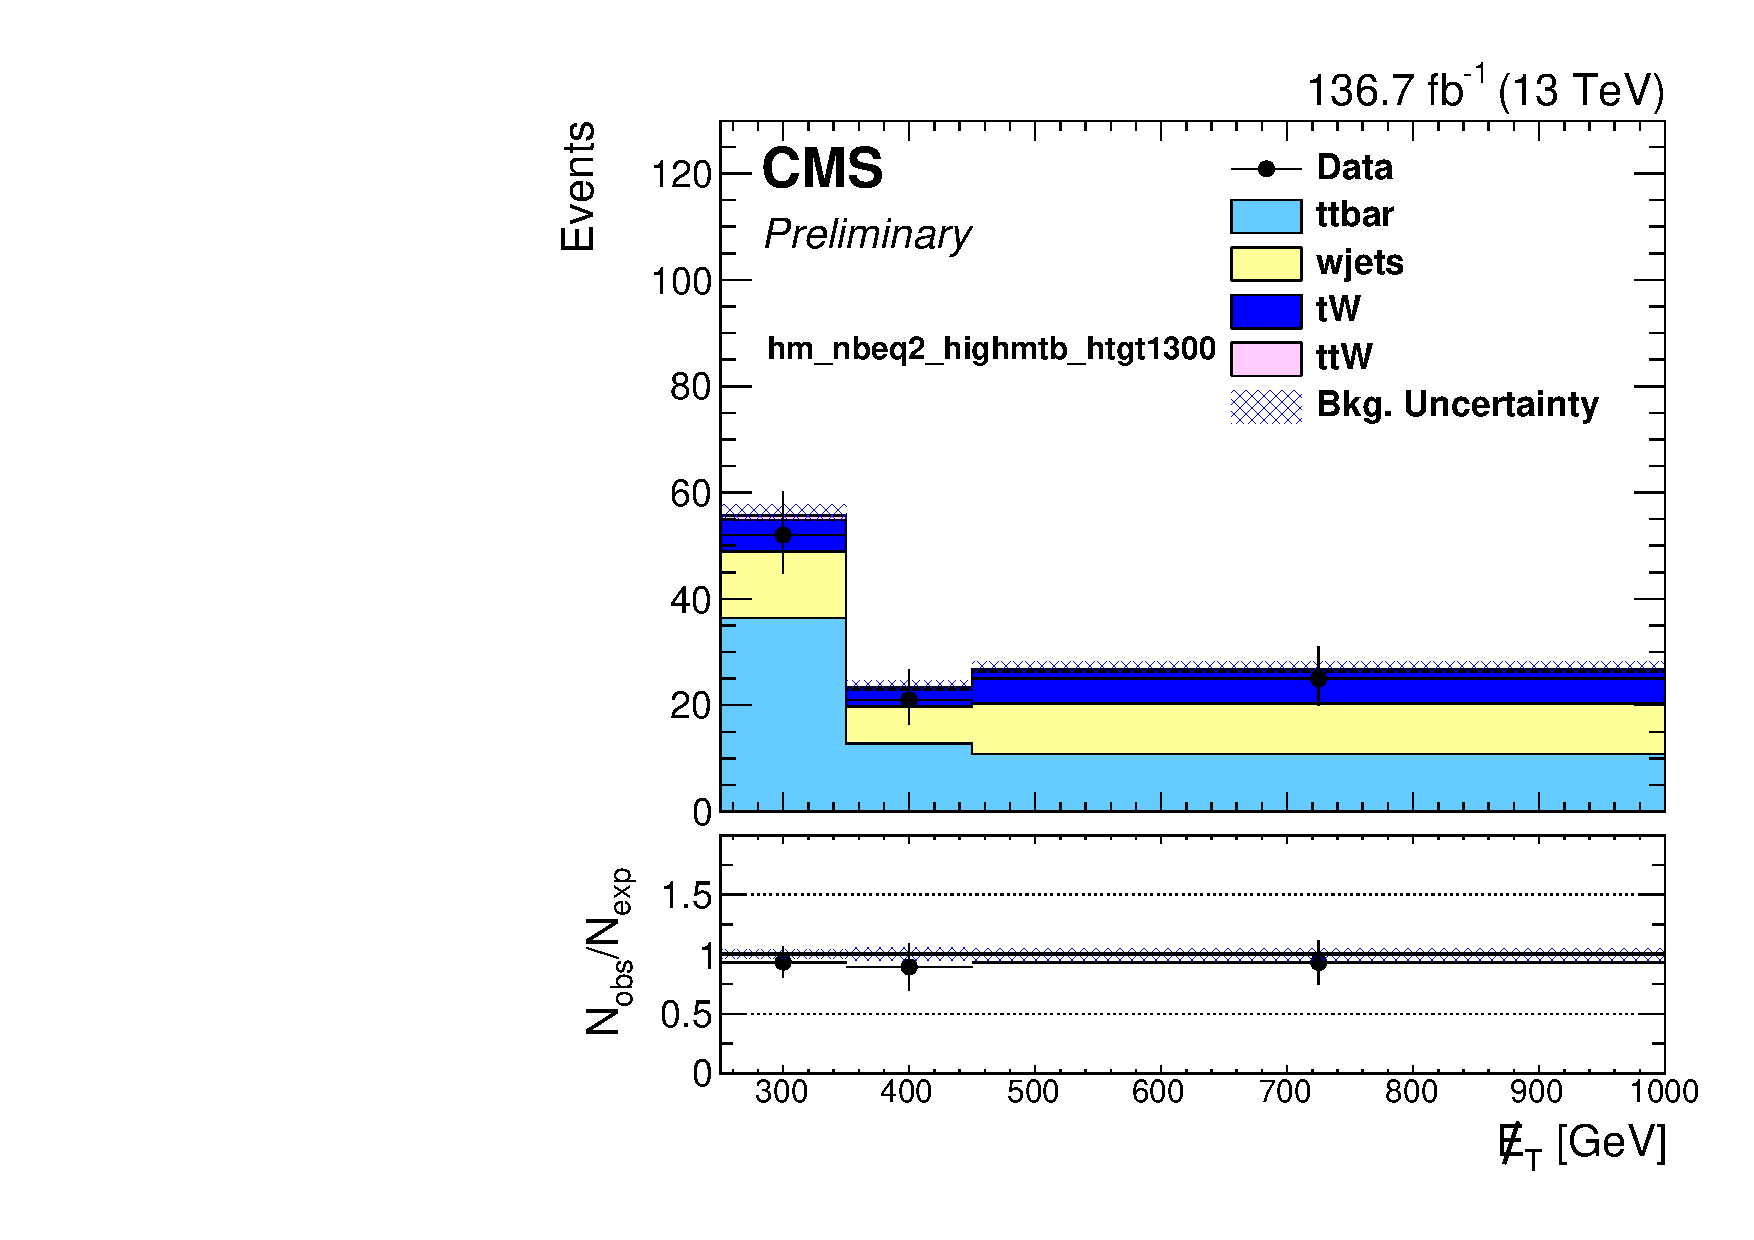
\includegraphics[width=0.32\textwidth]{../Research/SUSY/2019/LLB/lepcr_allEras/MET_pt_DataMC_hm_nbeq2_highmtb_nt0_nrt0_nw1_htgt1300__.pdf} \\
  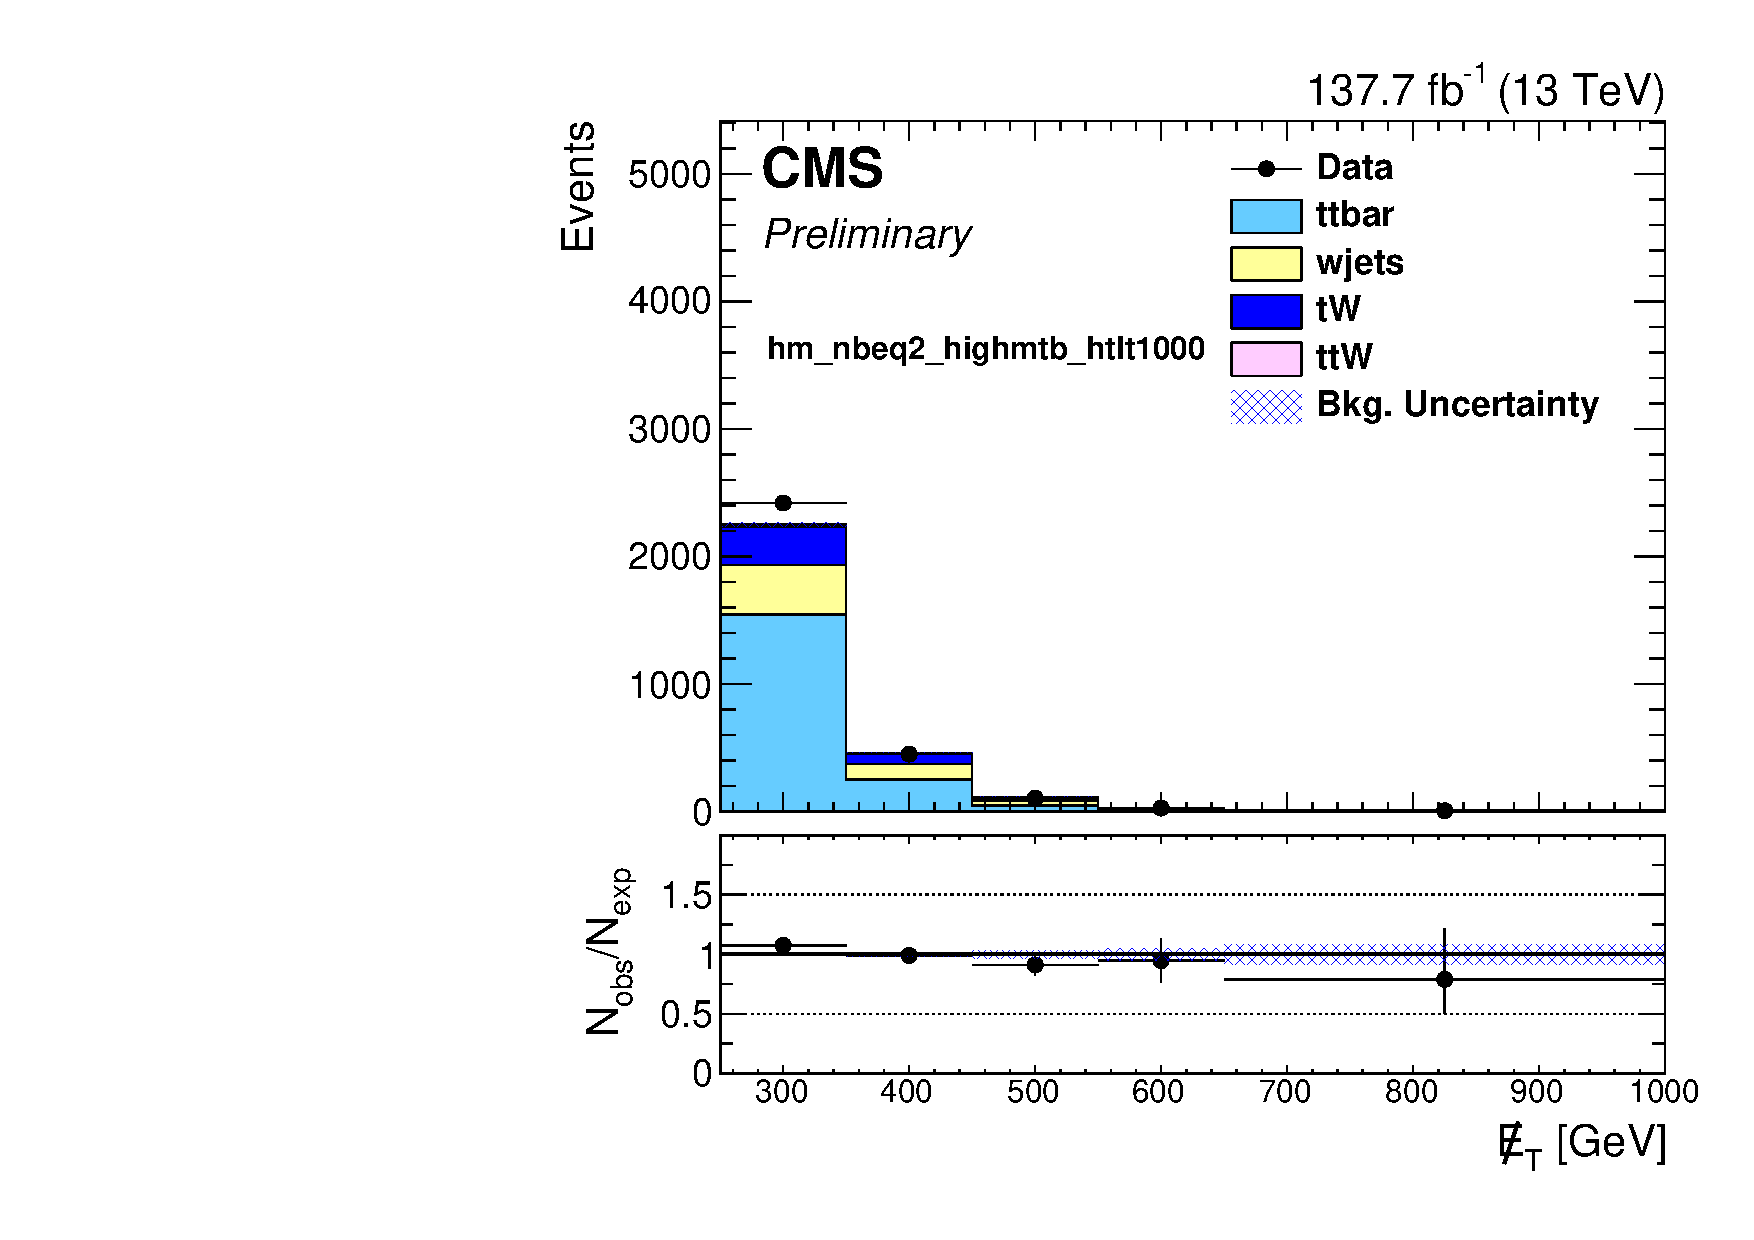
\includegraphics[width=0.32\textwidth]{../Research/SUSY/2019/LLB/lepcr_allEras/MET_pt_DataMC_hm_nbeq2_highmtb_nt0_nrt1_nw0_htlt1000__.pdf} 
  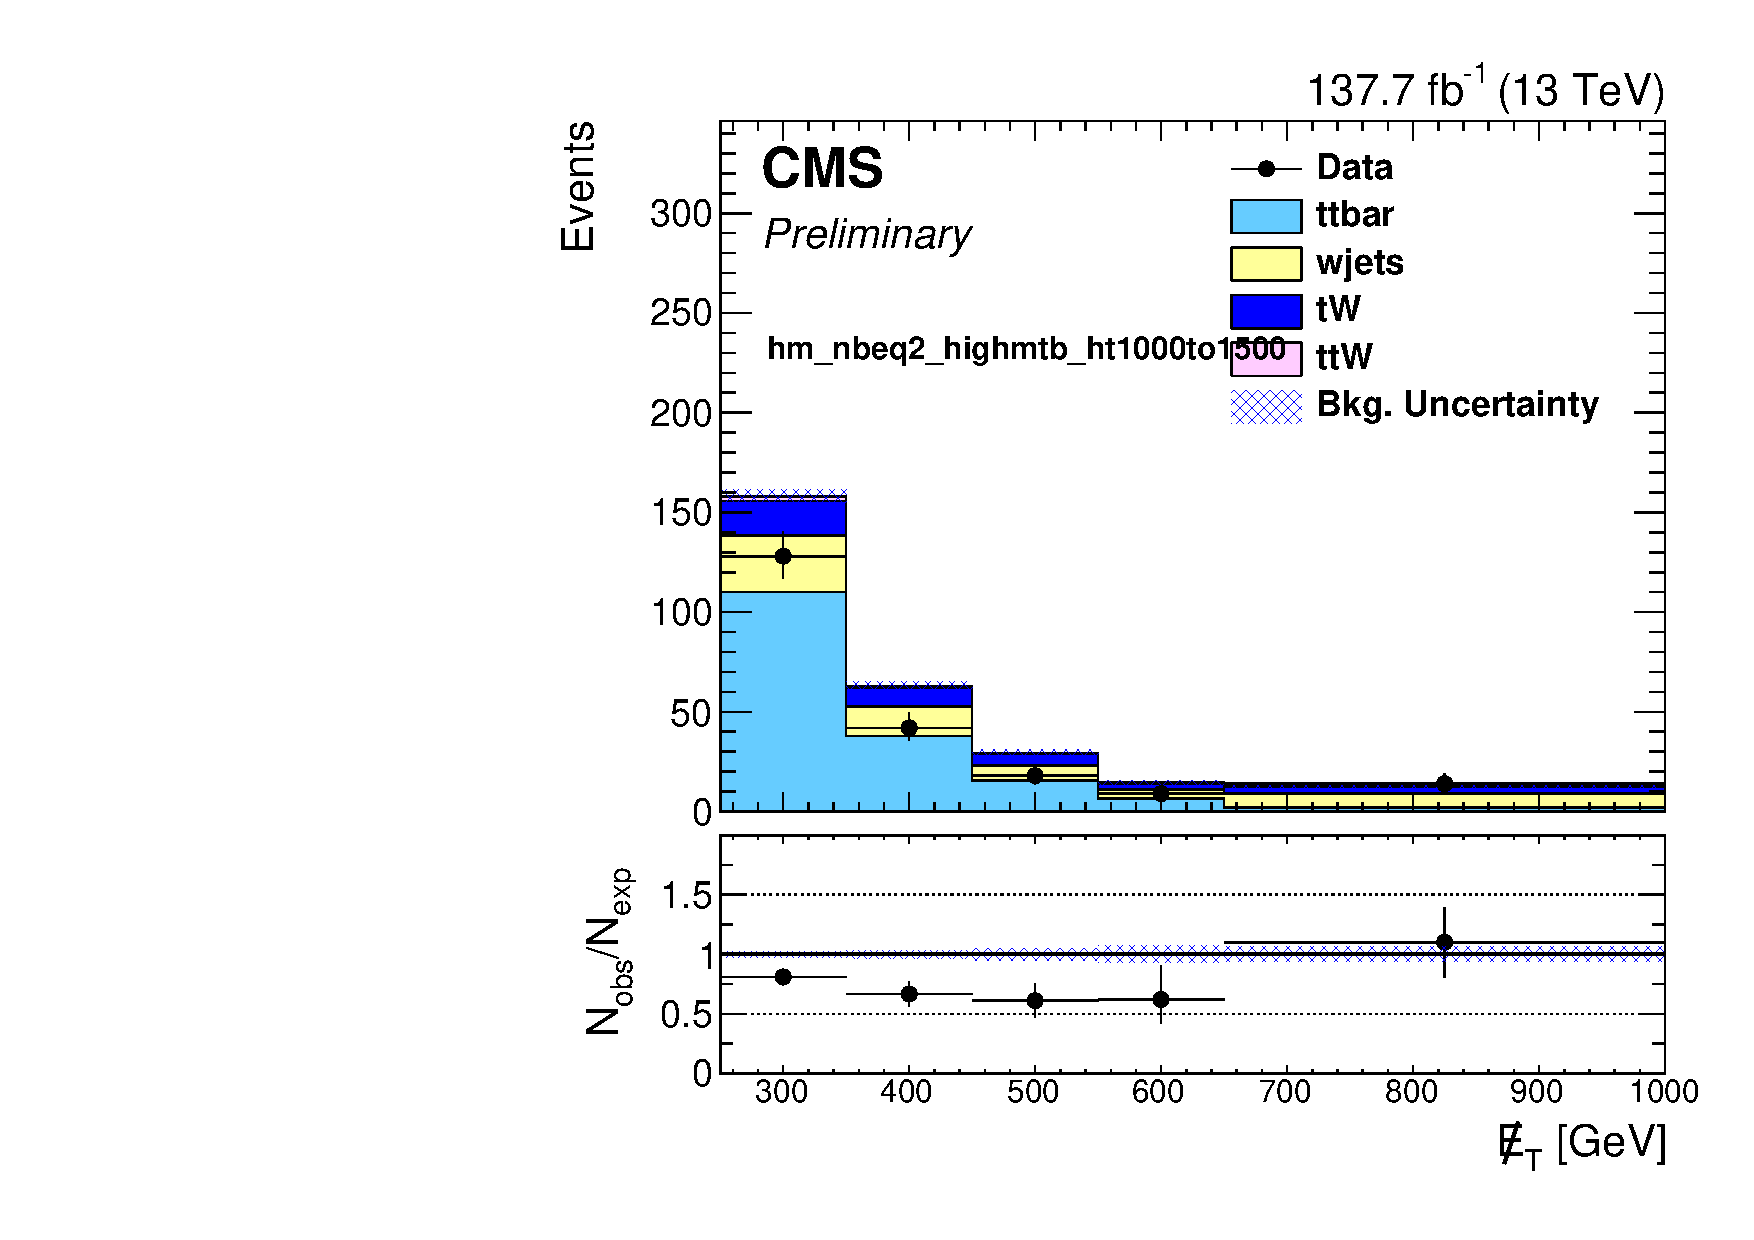
\includegraphics[width=0.32\textwidth]{../Research/SUSY/2019/LLB/lepcr_allEras/MET_pt_DataMC_hm_nbeq2_highmtb_nt0_nrt1_nw0_ht1000to1500__.pdf} 
  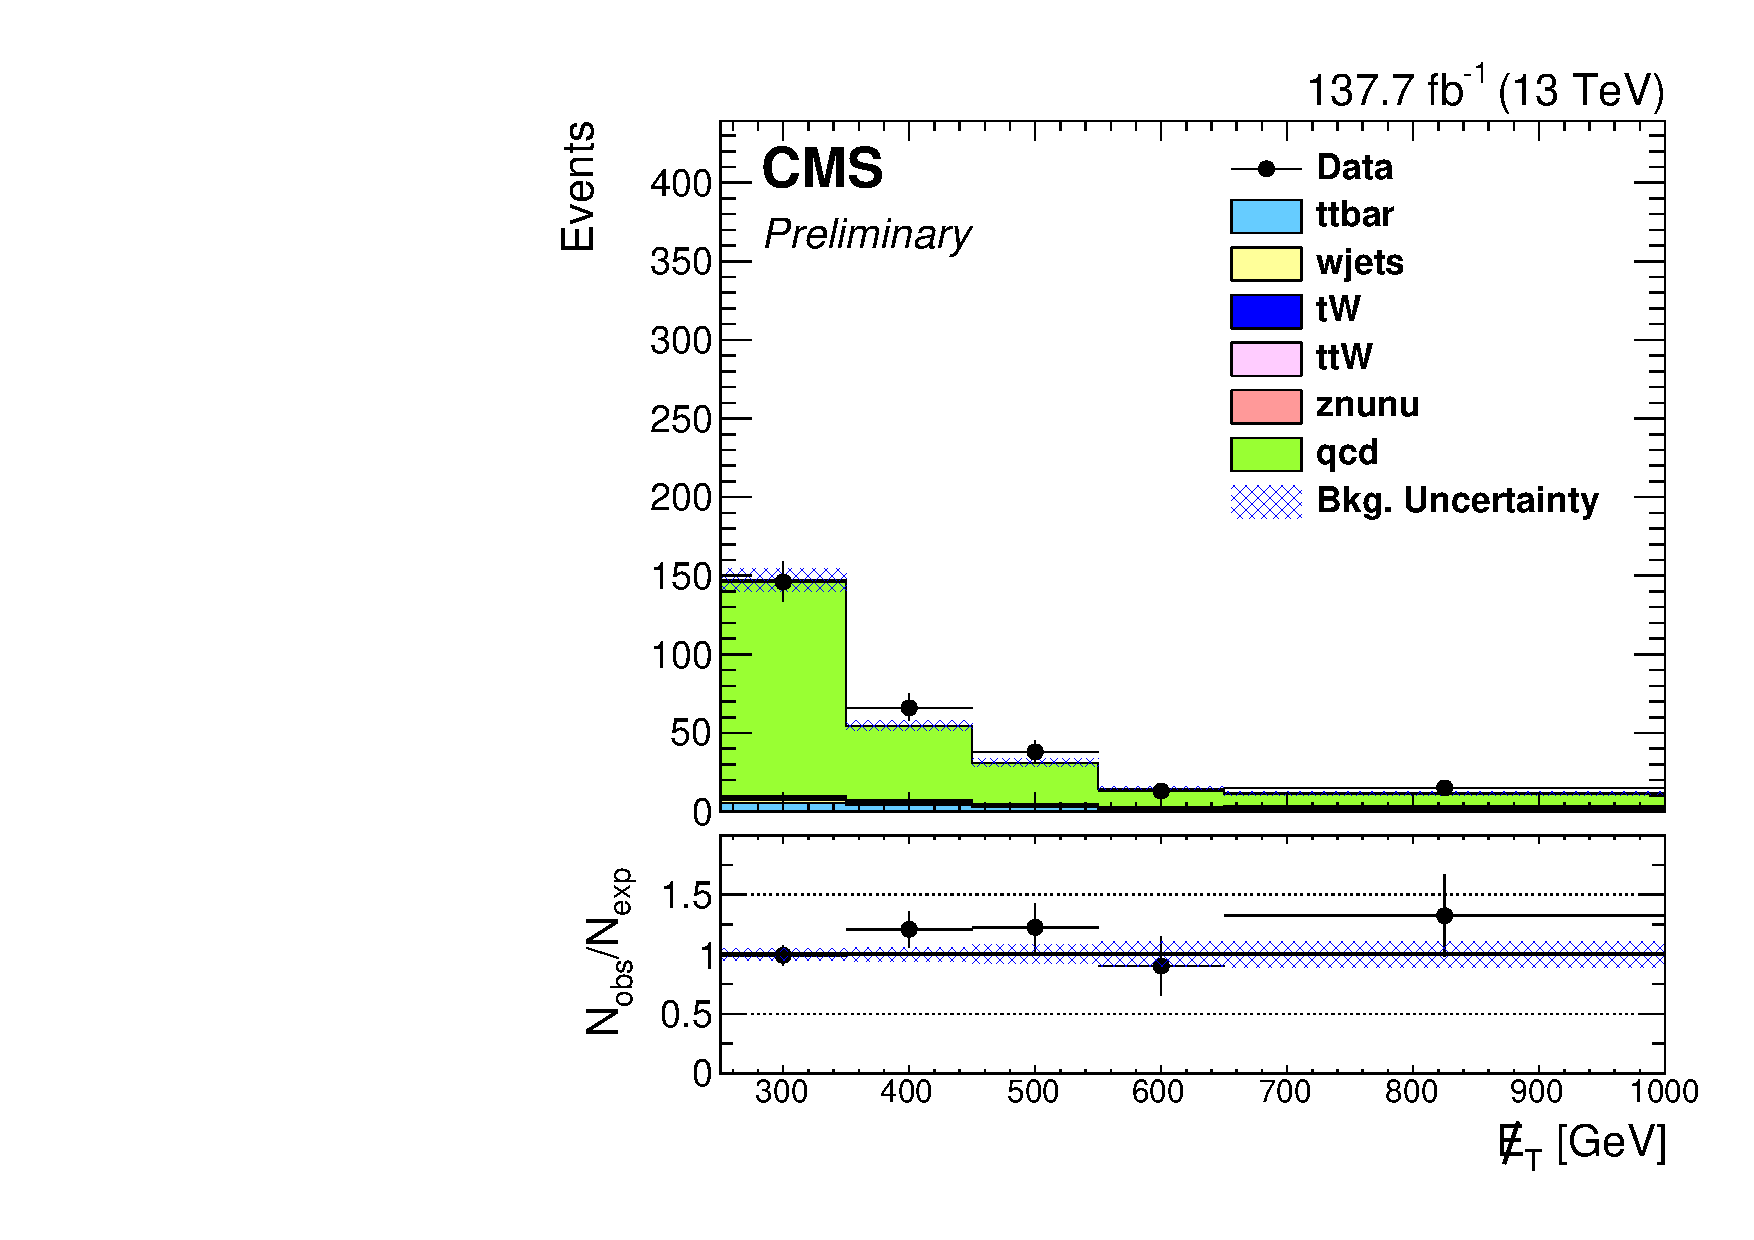
\includegraphics[width=0.32\textwidth]{../Research/SUSY/2019/LLB/lepcr_allEras/MET_pt_DataMC_hm_nbeq2_highmtb_nt0_nrt1_nw0_htgt1500__.pdf} \\
  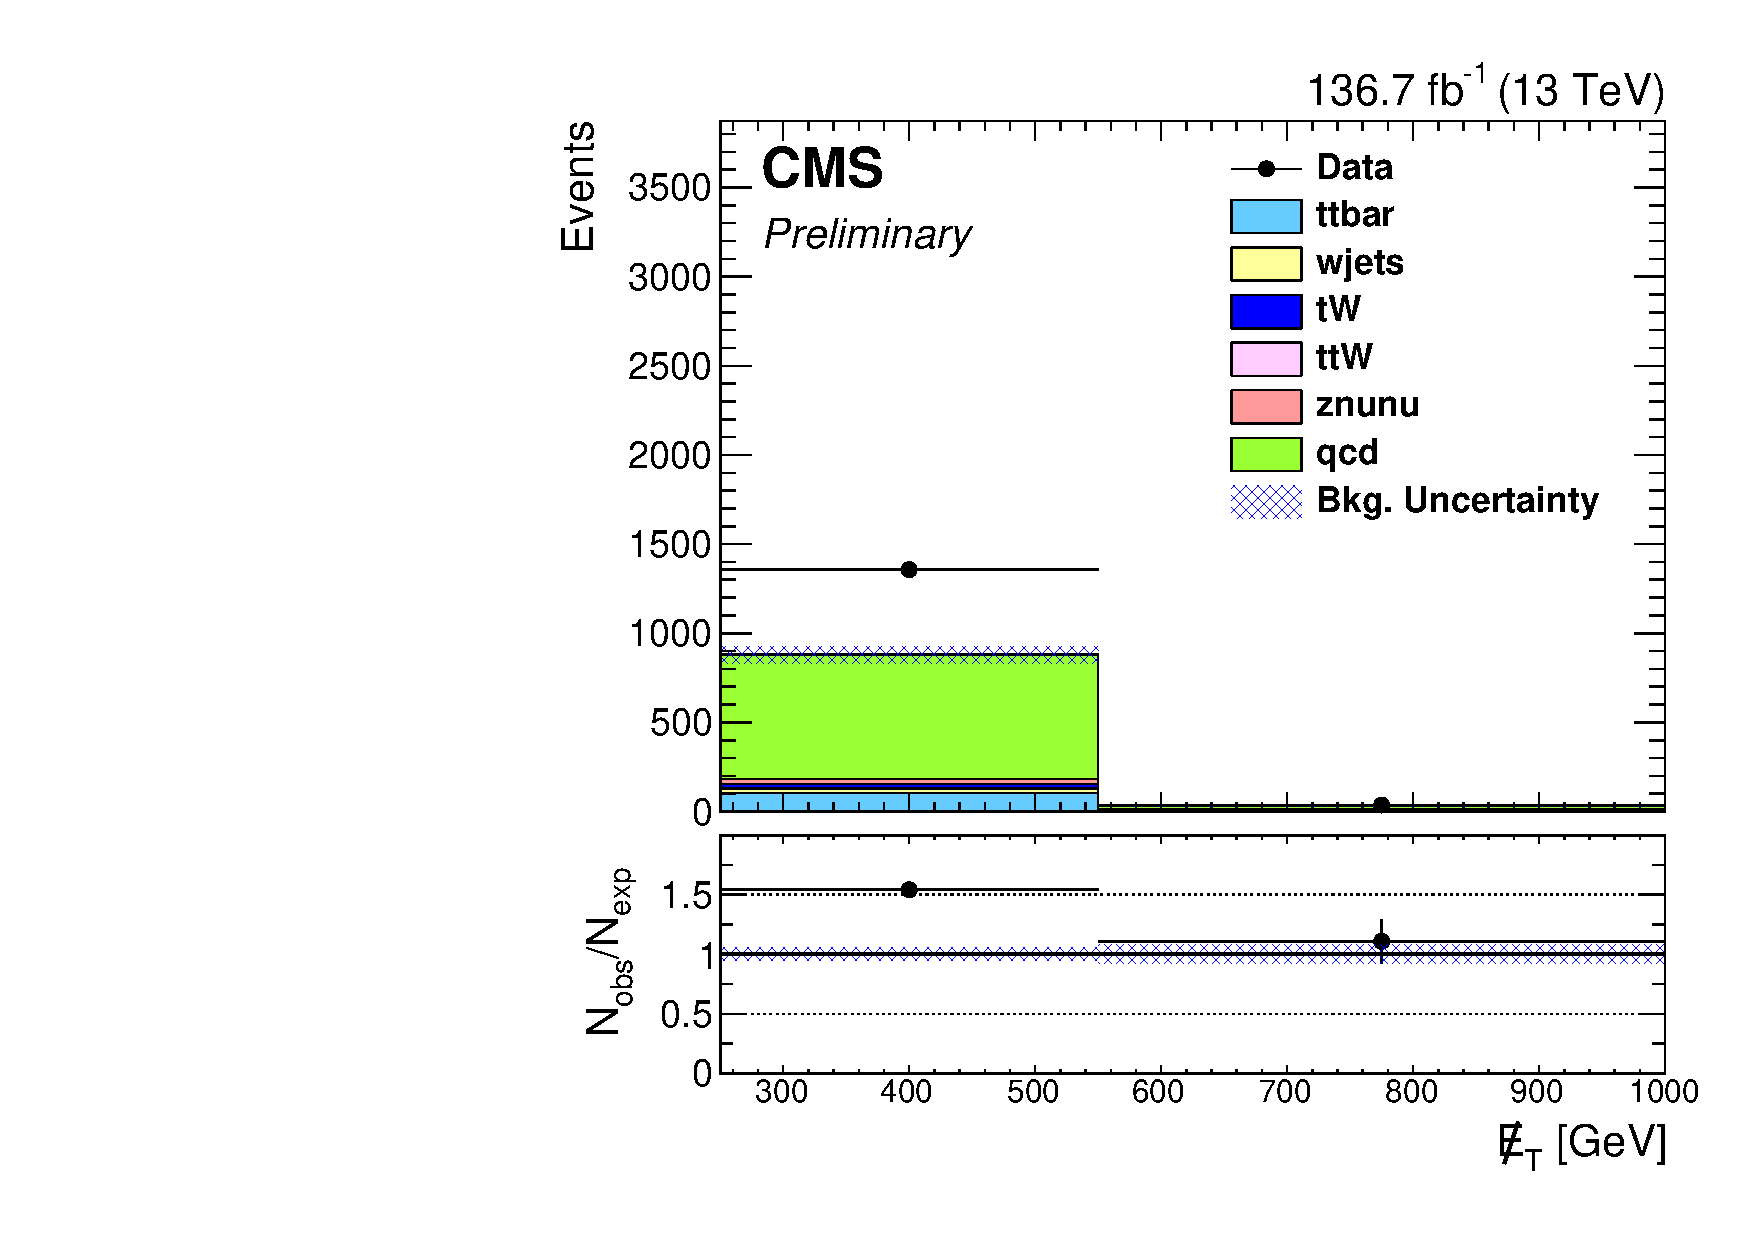
\includegraphics[width=0.32\textwidth]{../Research/SUSY/2019/LLB/lepcr_allEras/MET_pt_DataMC_hm_nbeq2_highmtb_nt1_nrt0_nw1__.pdf} 
  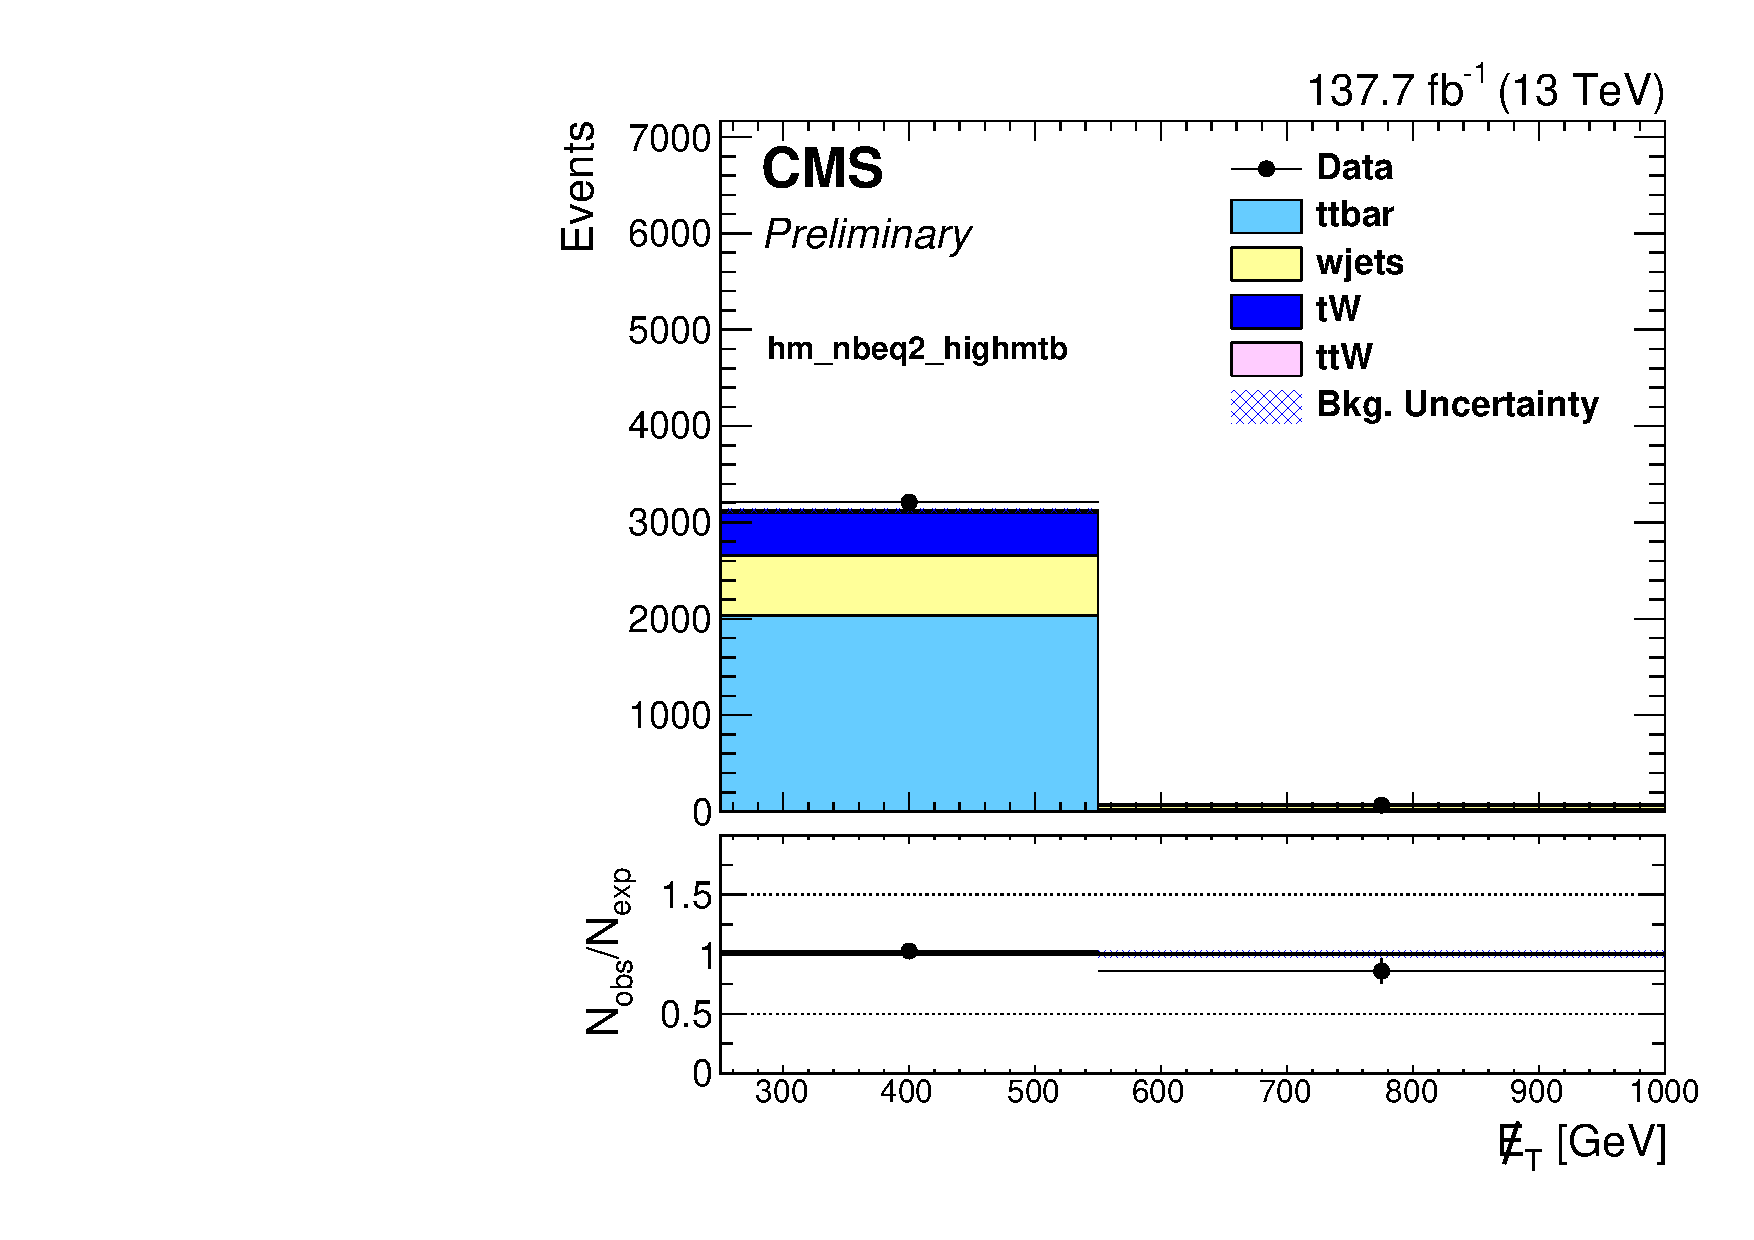
\includegraphics[width=0.32\textwidth]{../Research/SUSY/2019/LLB/lepcr_allEras/MET_pt_DataMC_hm_nbeq2_highmtb_nt0_nrt1_nw1__.pdf} \\
	\end{center}
	\caption{Comparison of the \met~distribution in the single-lepton sample after applying the high \dm~baseline selection in the $\nb=2$ and $\nt=1, \nrt=1,$ or $\nw=1$ regions. Data and simulation are represented by the black points and stacked histograms, respectively. The error bars on the ratio of observed data to simulation correspo    nd to the data statistical uncertainty and the shaded blue band represents the statistical uncertainty on the simulation. These regions are included with the search regions in the simultaneous fit for the signal extraction in order to estimate the LL contribution.
	 %               The plots in the top row are for events with $\mtb<175$~\GeV, with $5\leq\nj<7$ on the left and $\nj\geq7$ on the right. 
	 %               The plots in the middle row are for events with $\mtb>175$~\GeV and $\nt=0, \nw=0$, with $5\leq\nj<7$ on the left and $\nj\geq7$ on the right. 
	 %               The plot in the bottom row is for events with $\mtb>175$~\GeV and $\nj\geq5$, with $\nt=0, \nw\geq1$ on the left, $\nt\geq1, \nw=0$ on the middle, and $\nt\geq1$, and $\nw\geq1$ on the right.
	 }
	\label{fig:llb-1lcr-datavsmc-hm-nb2-1}
\end{figure}

\begin{figure}[!htb]
	\begin{center}
  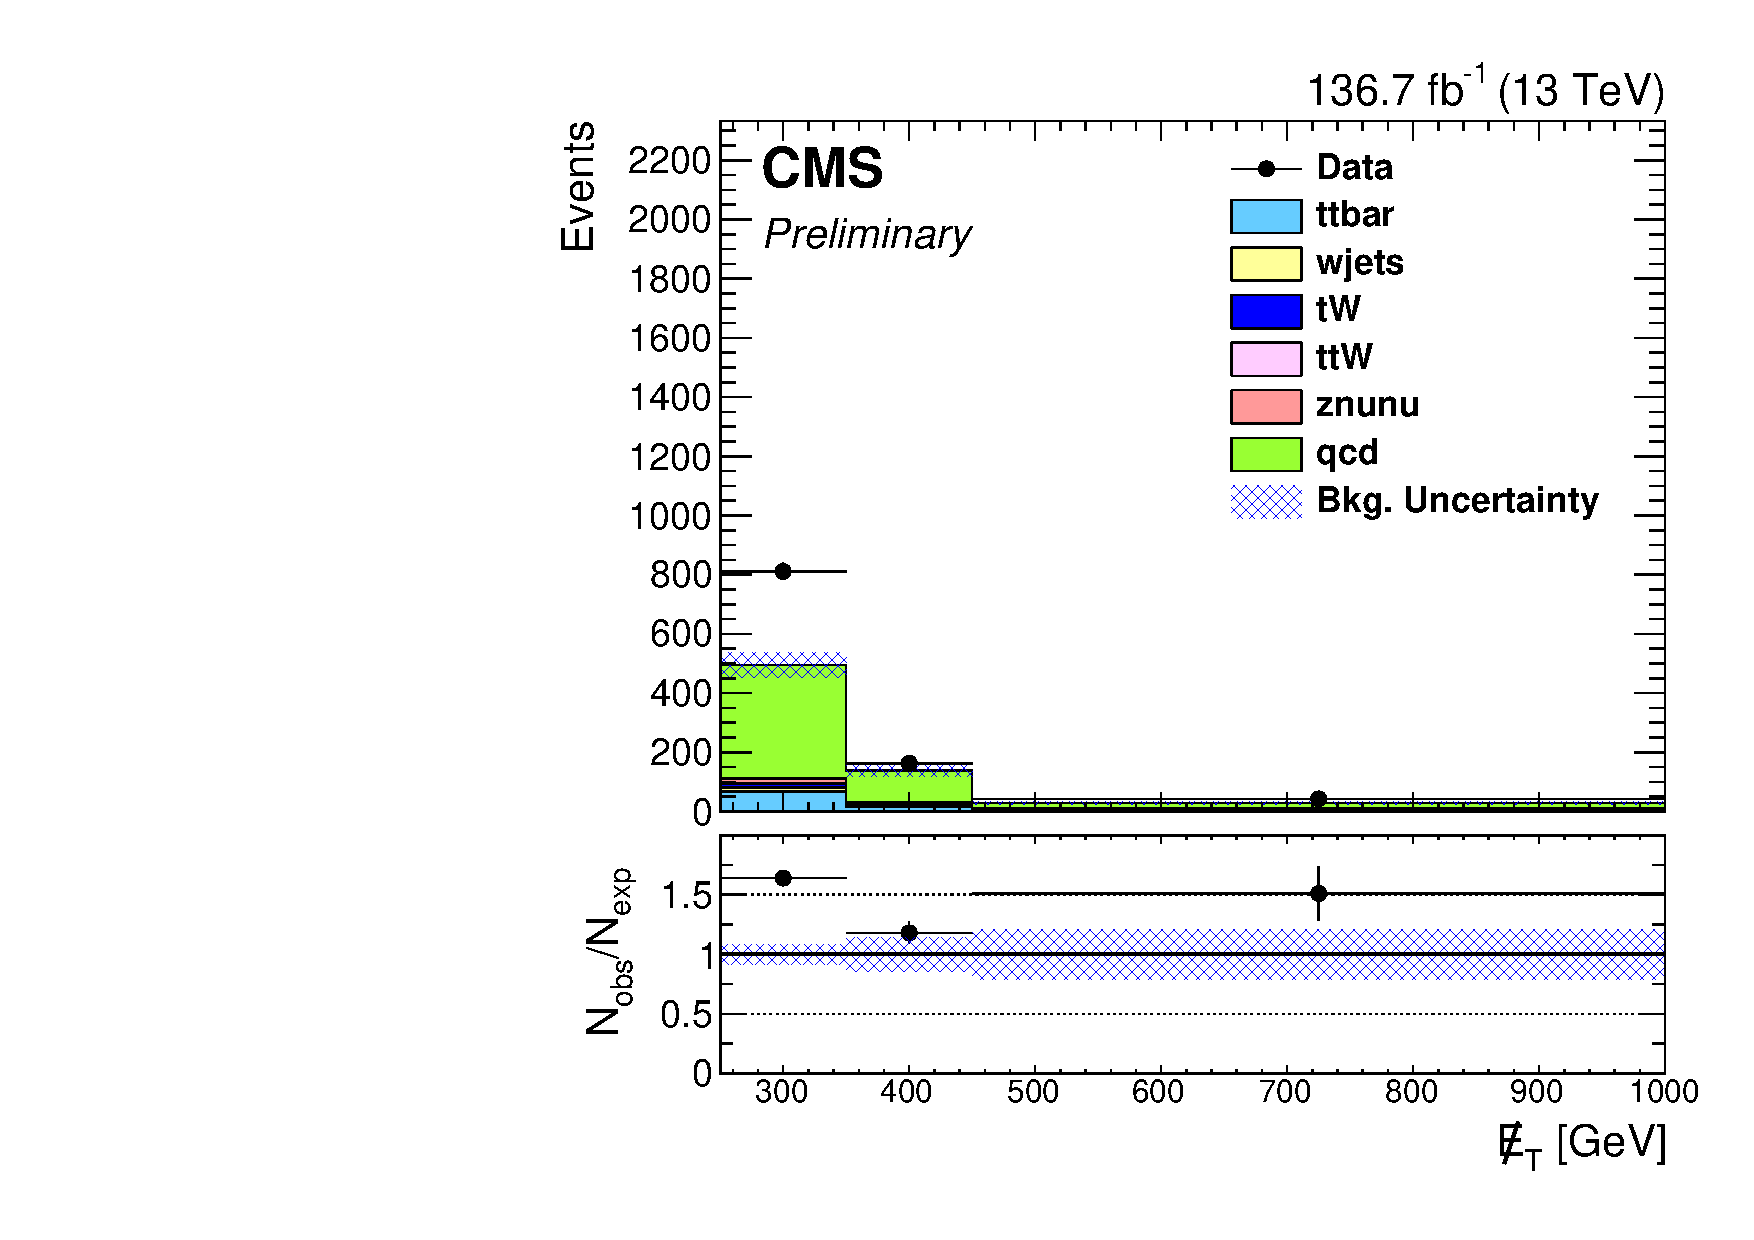
\includegraphics[width=0.32\textwidth]{../Research/SUSY/2019/LLB/lepcr_allEras/MET_pt_DataMC_hm_nbeq2_highmtb_nt1_nrt1_nw0_htlt1300__.pdf}
  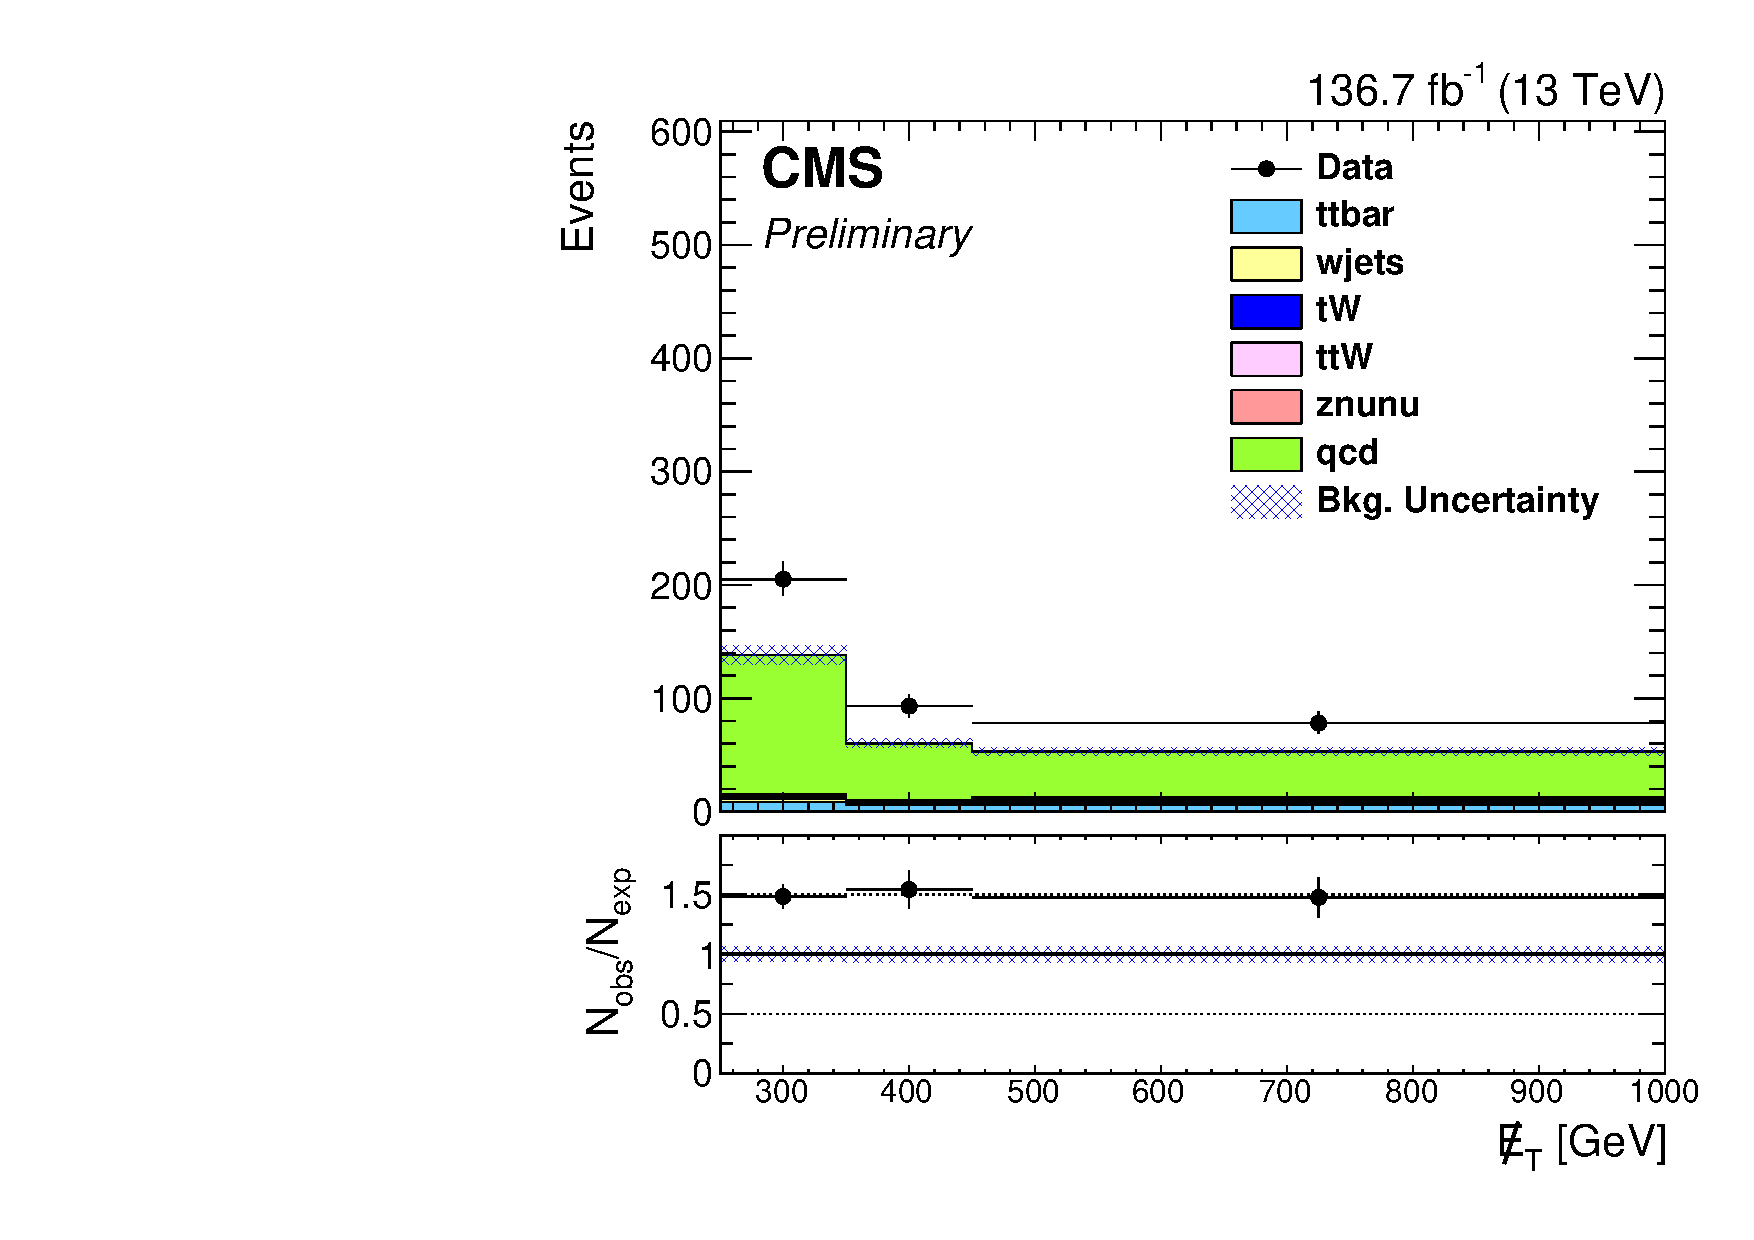
\includegraphics[width=0.32\textwidth]{../Research/SUSY/2019/LLB/lepcr_allEras/MET_pt_DataMC_hm_nbeq2_highmtb_nt1_nrt1_nw0_htgt1300__.pdf} \\
  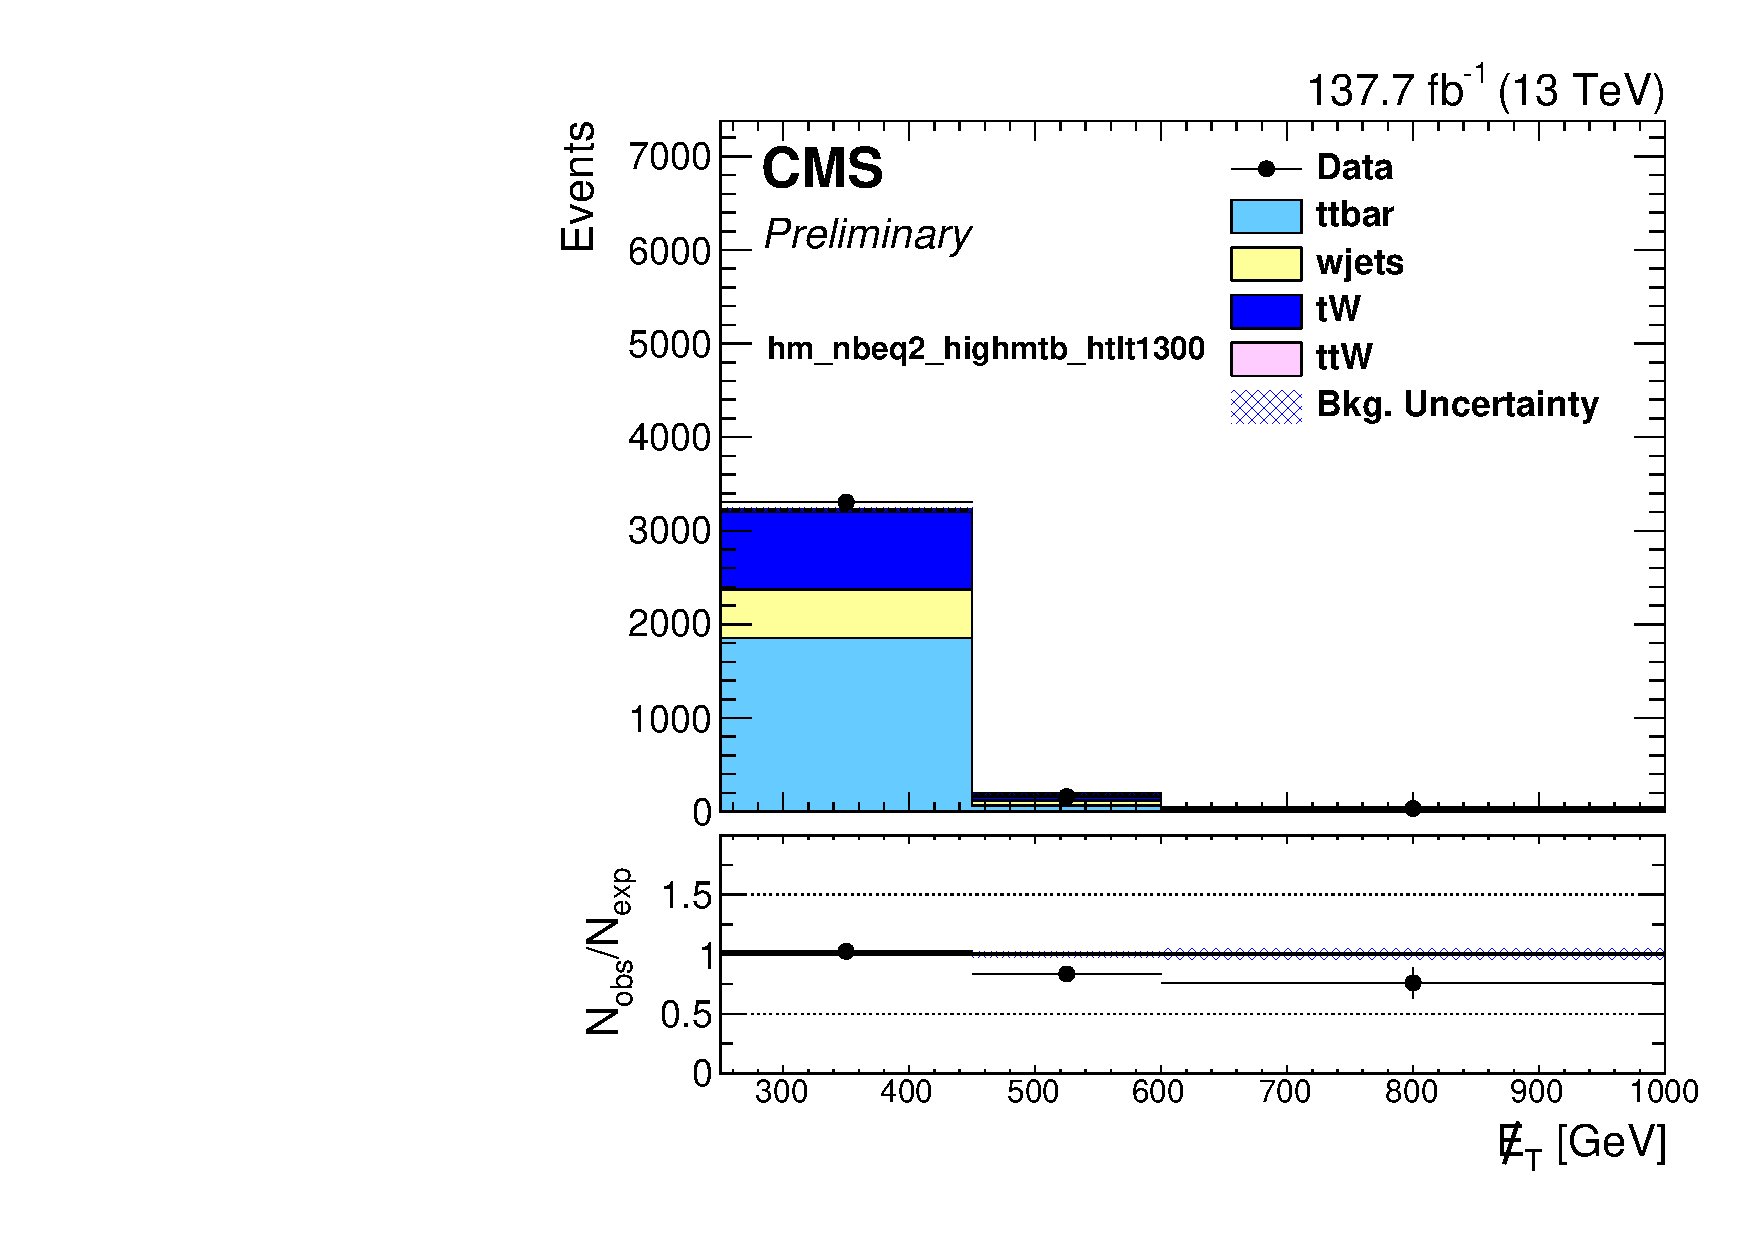
\includegraphics[width=0.32\textwidth]{../Research/SUSY/2019/LLB/lepcr_allEras/MET_pt_DataMC_hm_nbeq2_highmtb_nt2_nrt0_nw0_htlt1300__.pdf}
  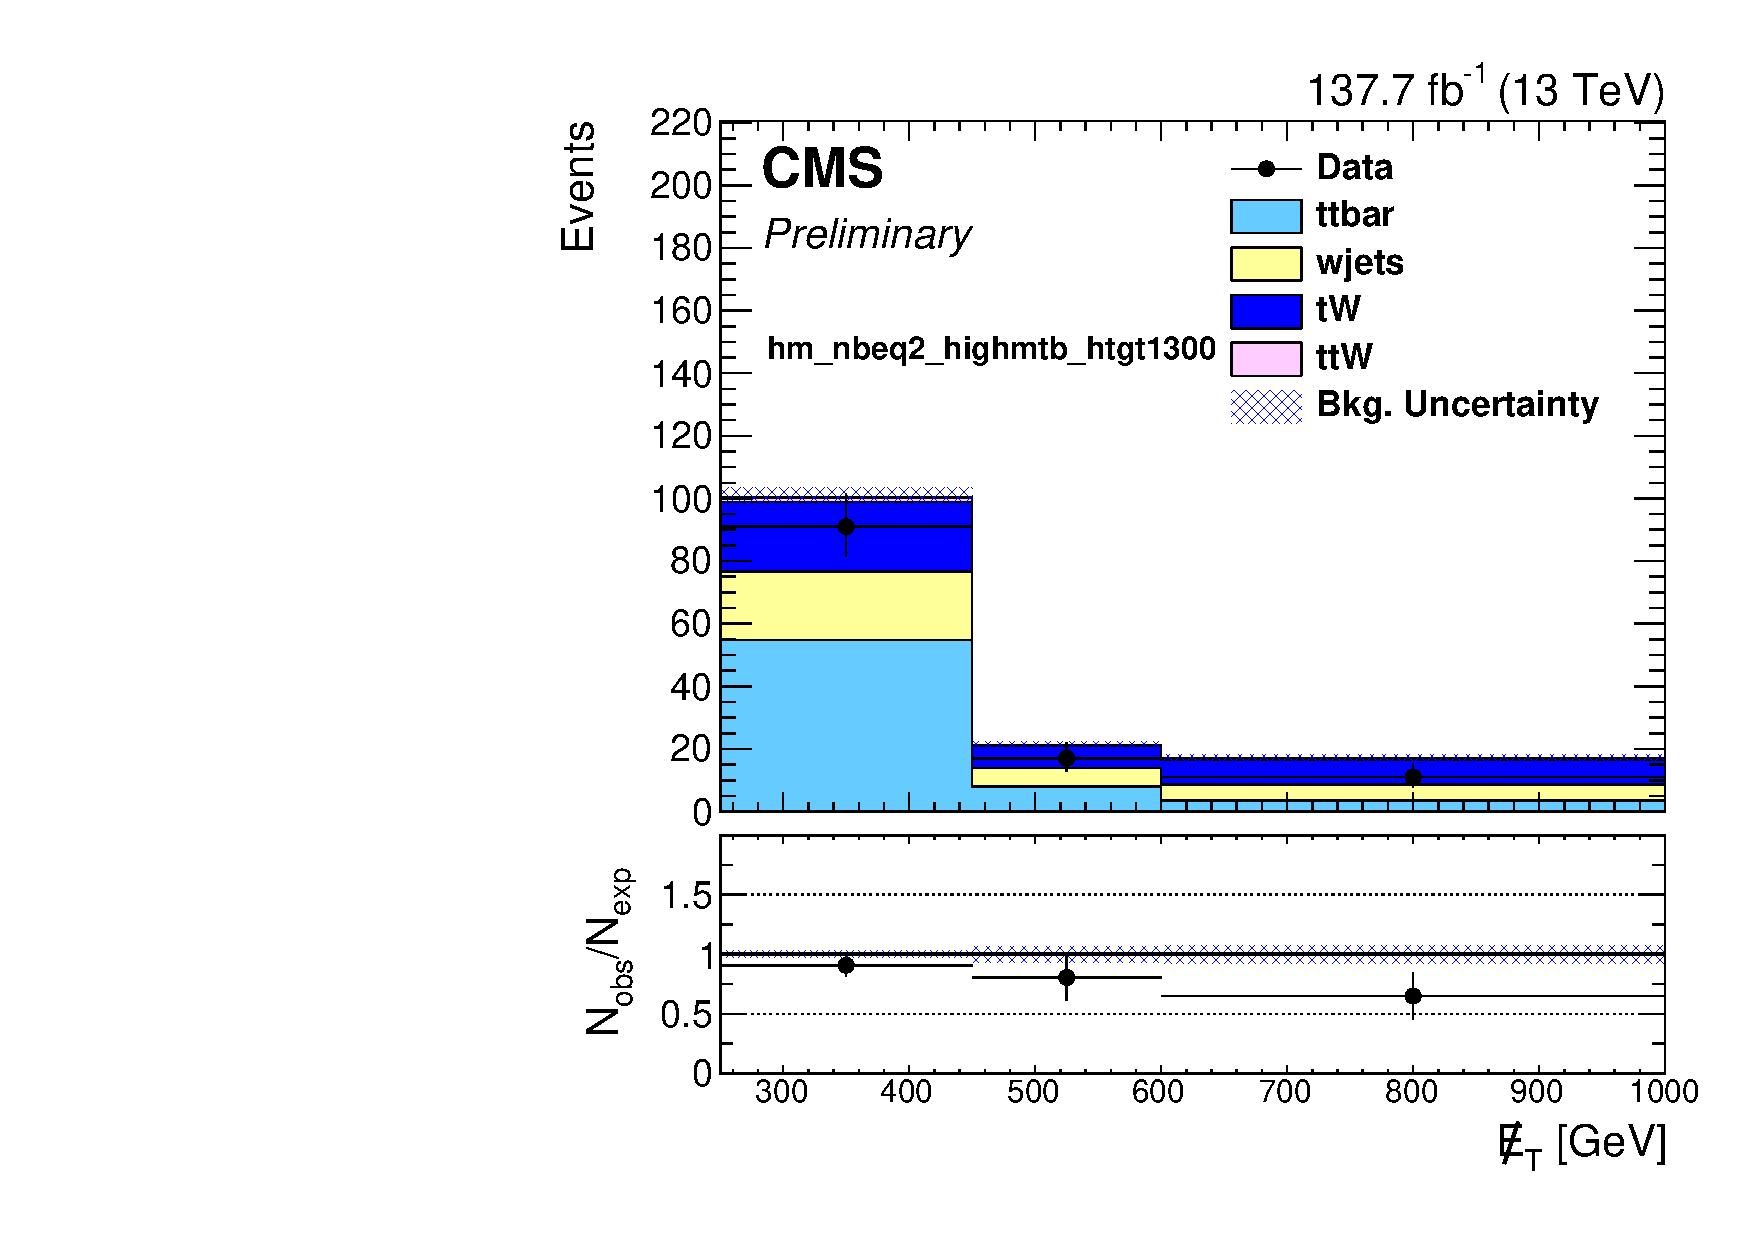
\includegraphics[width=0.32\textwidth]{../Research/SUSY/2019/LLB/lepcr_allEras/MET_pt_DataMC_hm_nbeq2_highmtb_nt2_nrt0_nw0_htgt1300__.pdf} 
  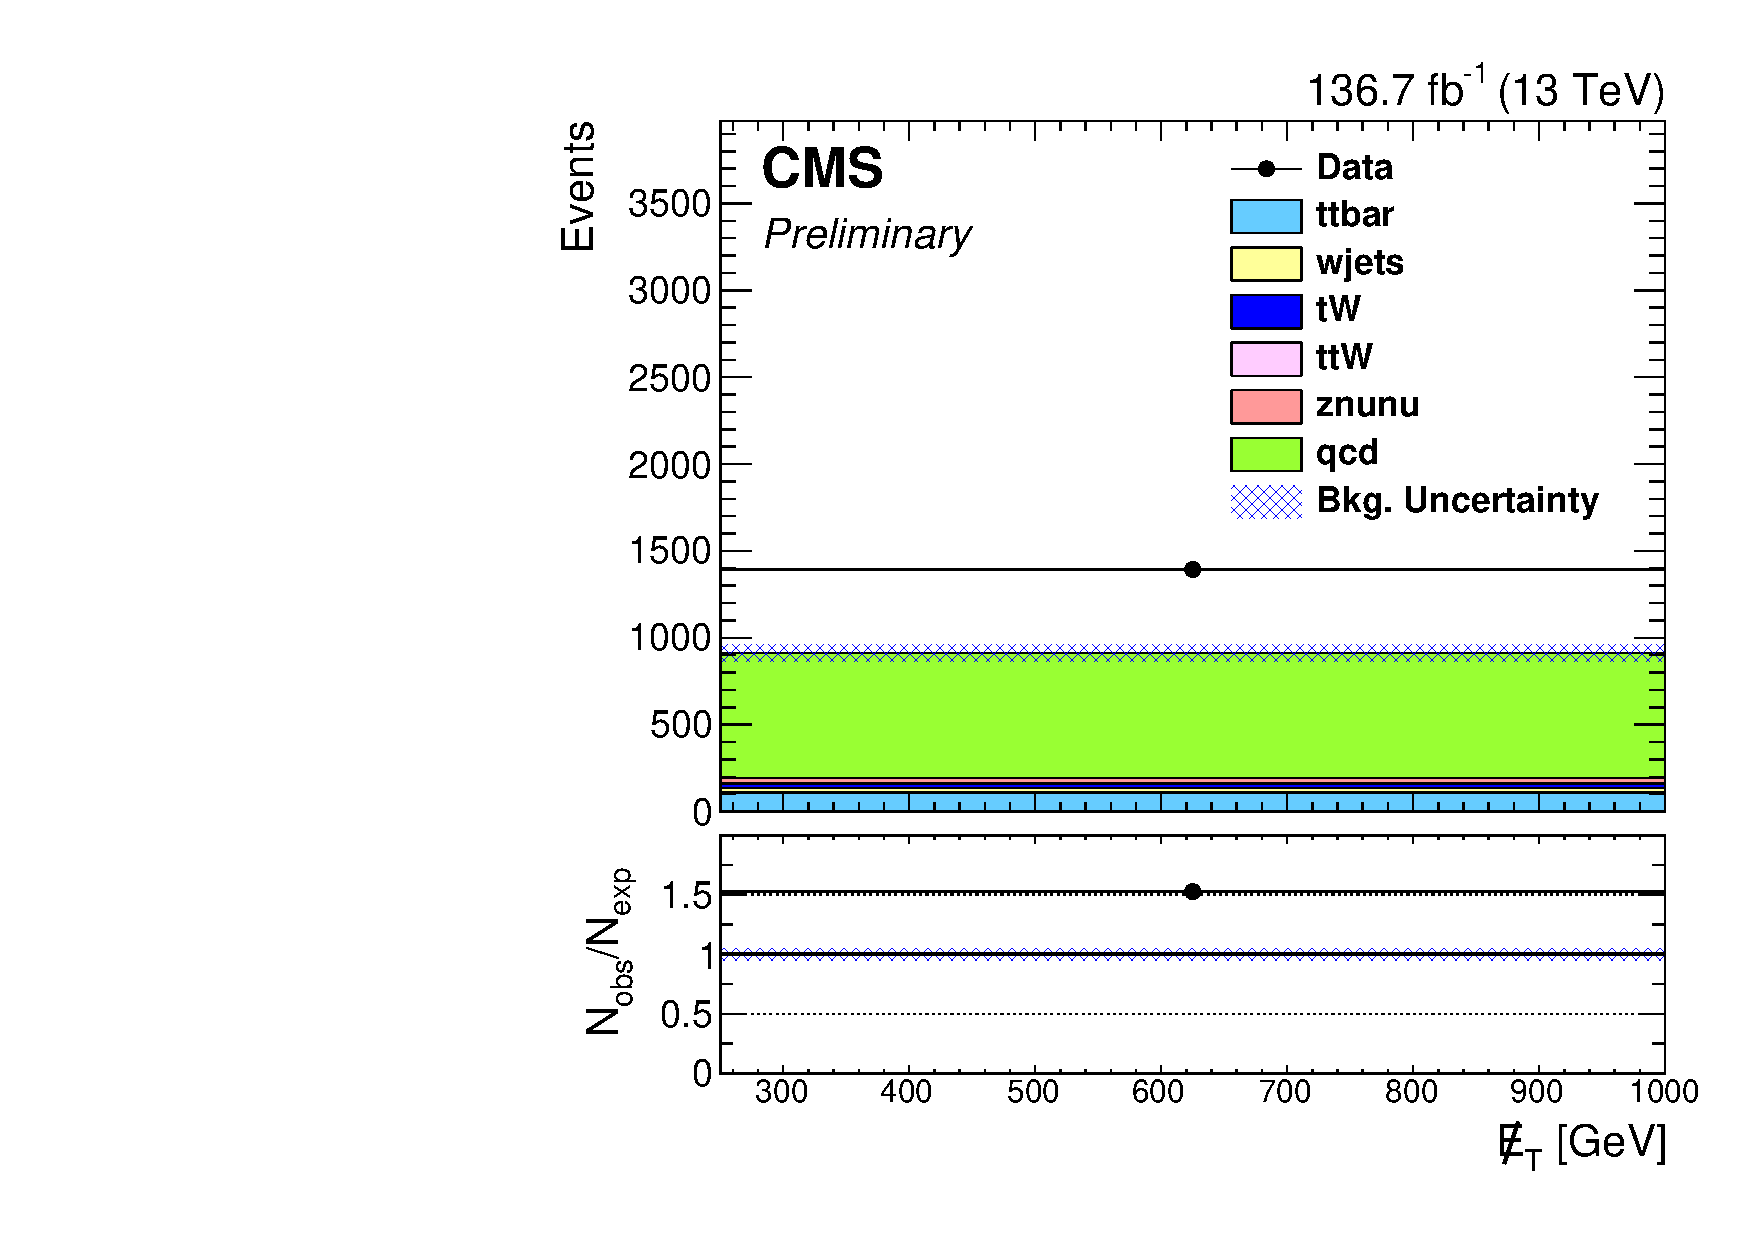
\includegraphics[width=0.32\textwidth]{../Research/SUSY/2019/LLB/lepcr_allEras/MET_pt_DataMC_hm_nbeq2_highmtb_nt0_nrt0_nw2__.pdf} \\
  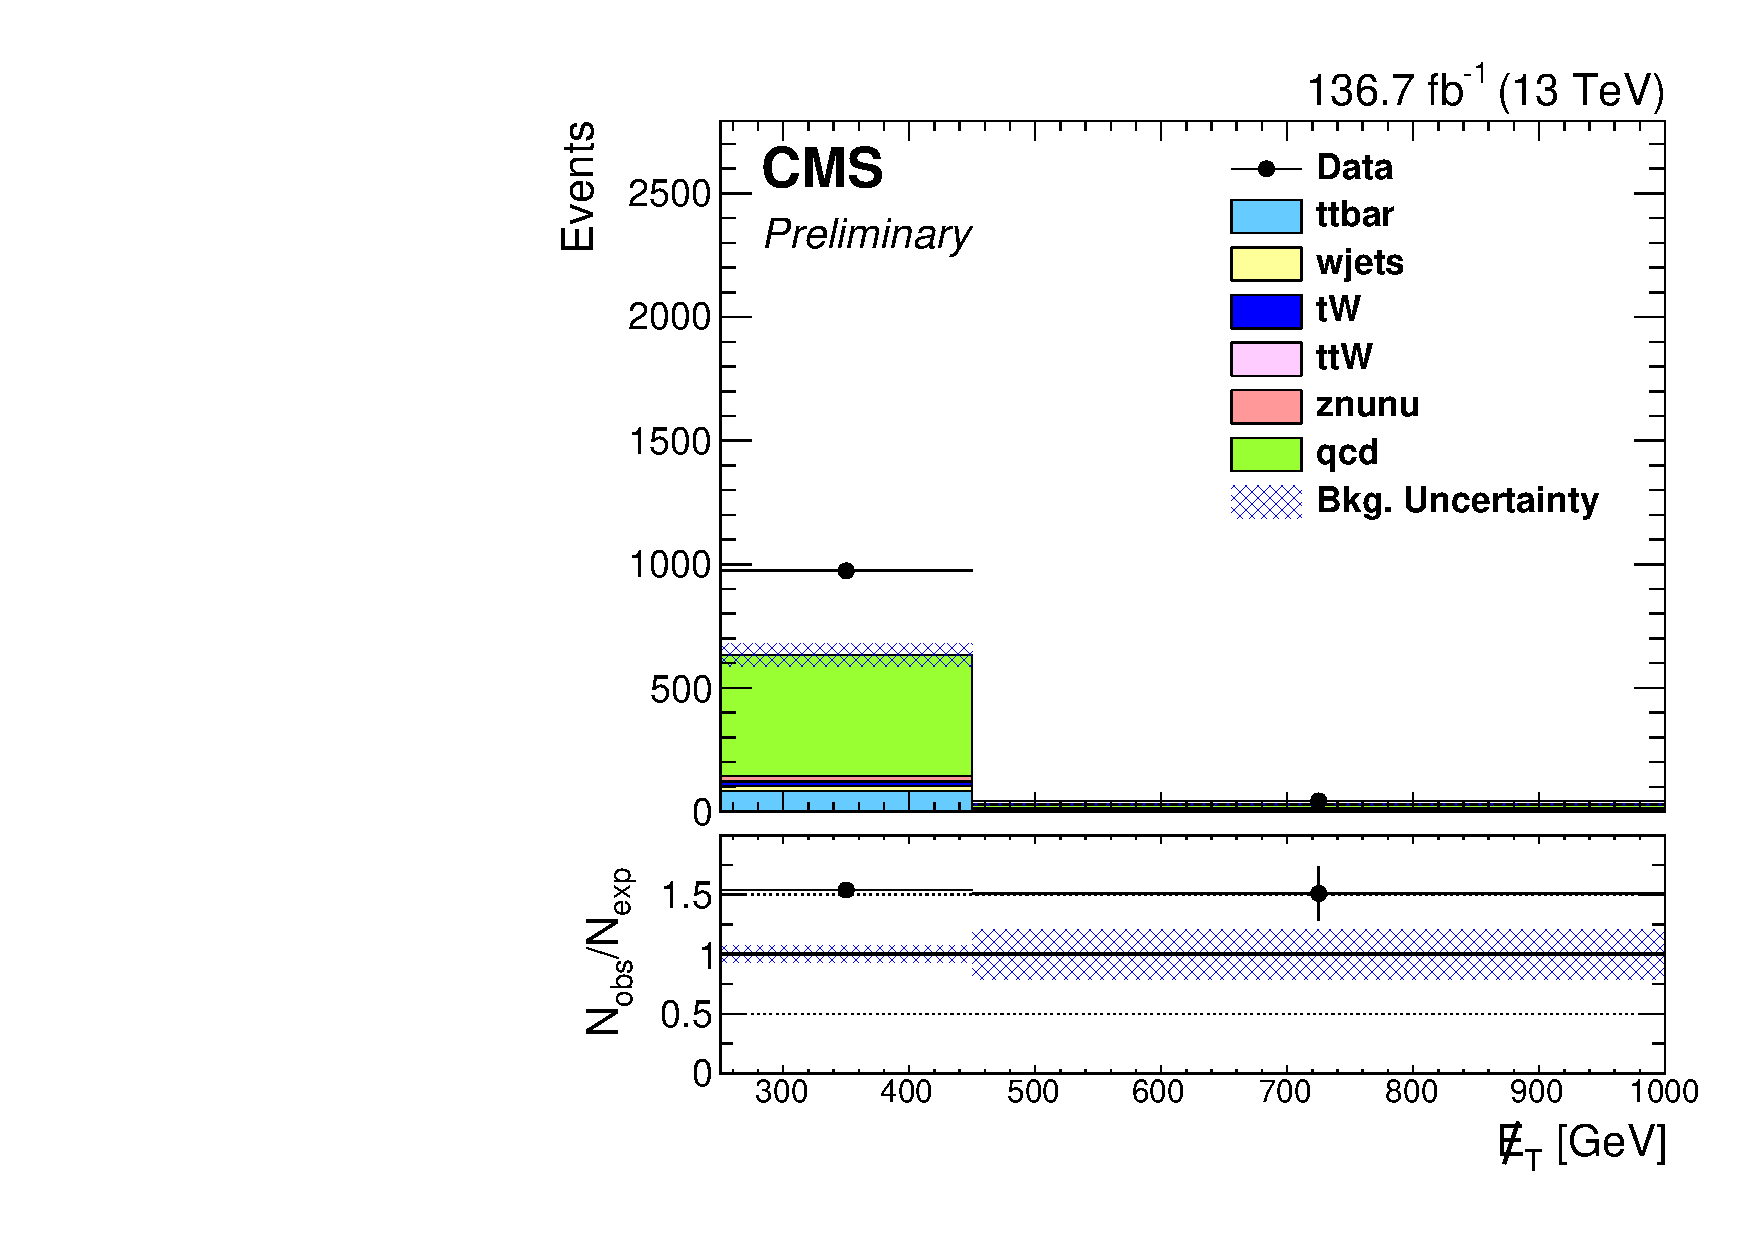
\includegraphics[width=0.32\textwidth]{../Research/SUSY/2019/LLB/lepcr_allEras/MET_pt_DataMC_hm_nbeq2_highmtb_nt0_nrt2_nw0_htlt1300__.pdf}  
  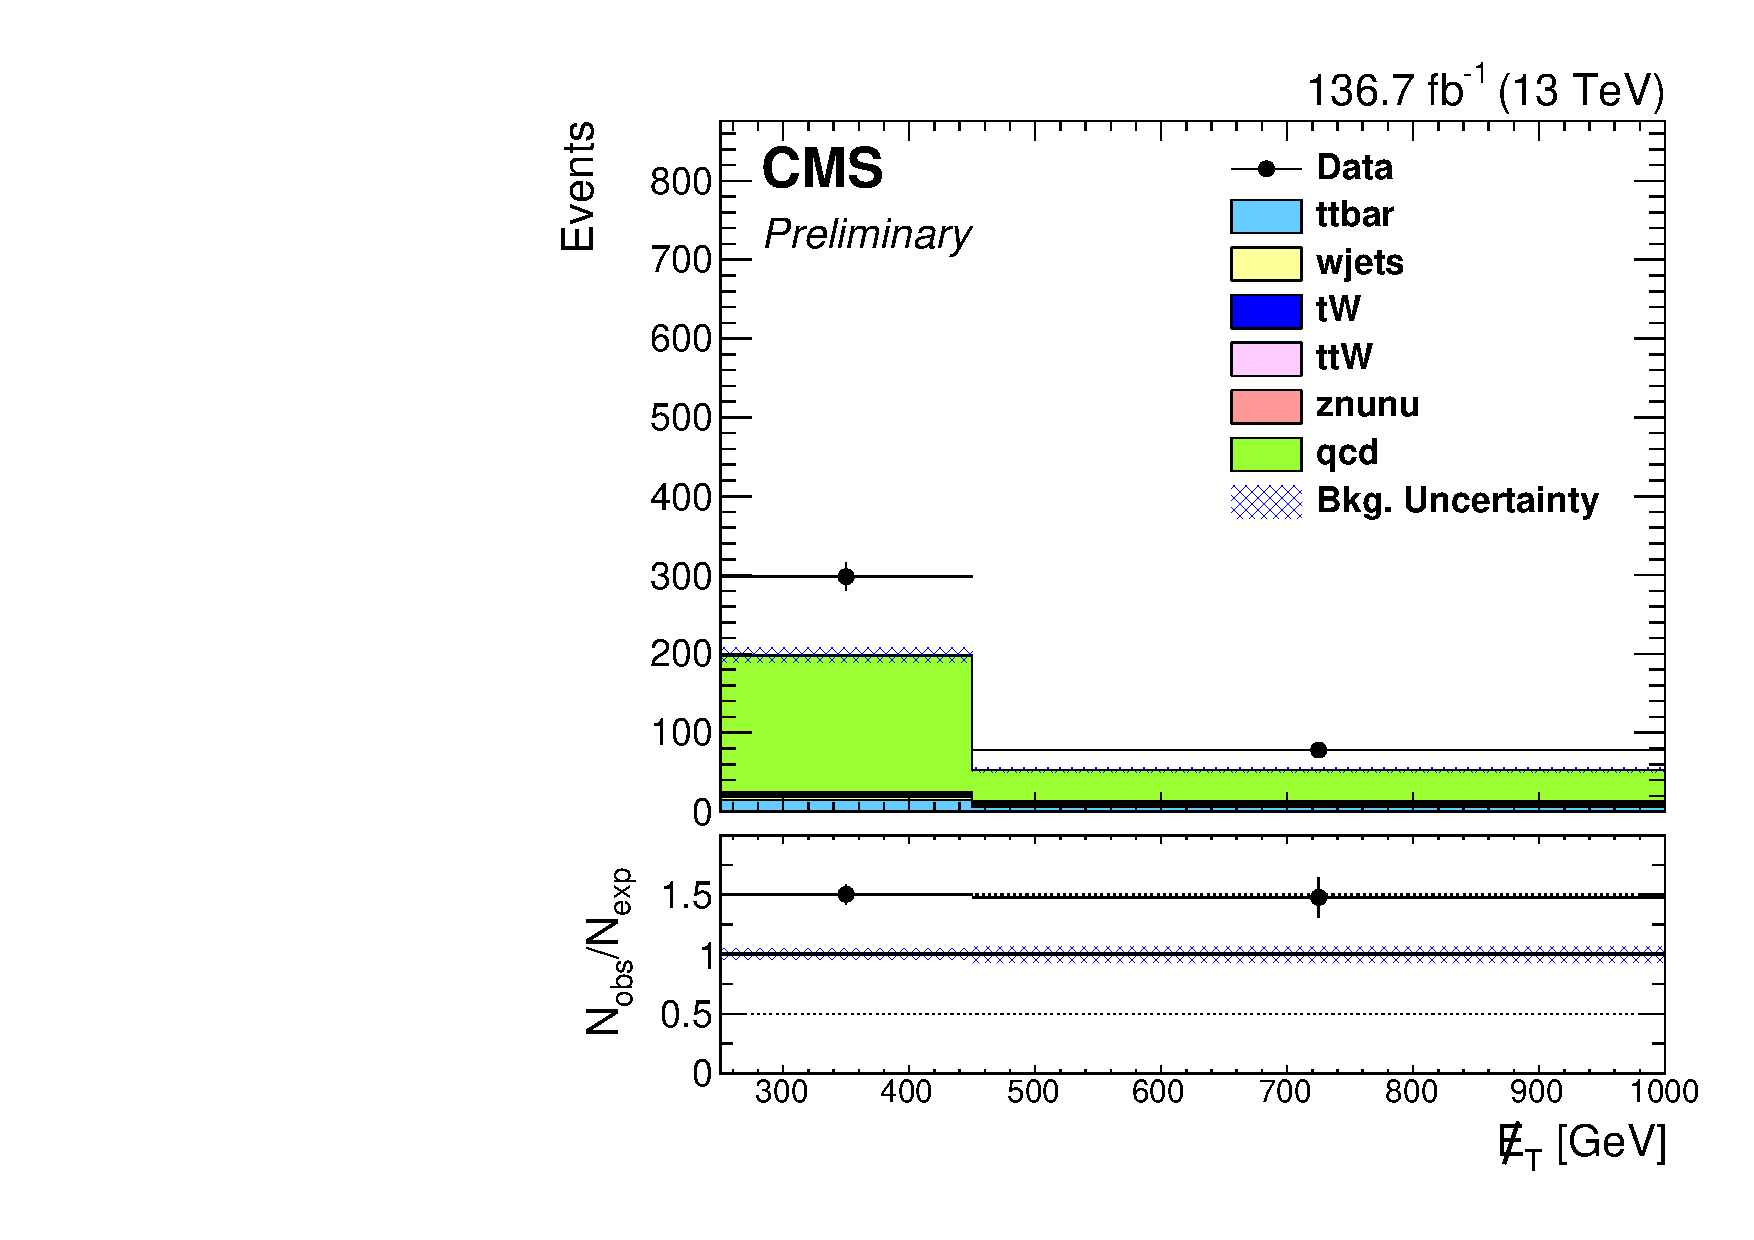
\includegraphics[width=0.32\textwidth]{../Research/SUSY/2019/LLB/lepcr_allEras/MET_pt_DataMC_hm_nbeq2_highmtb_nt0_nrt2_nw0_htgt1300__.pdf} \\
  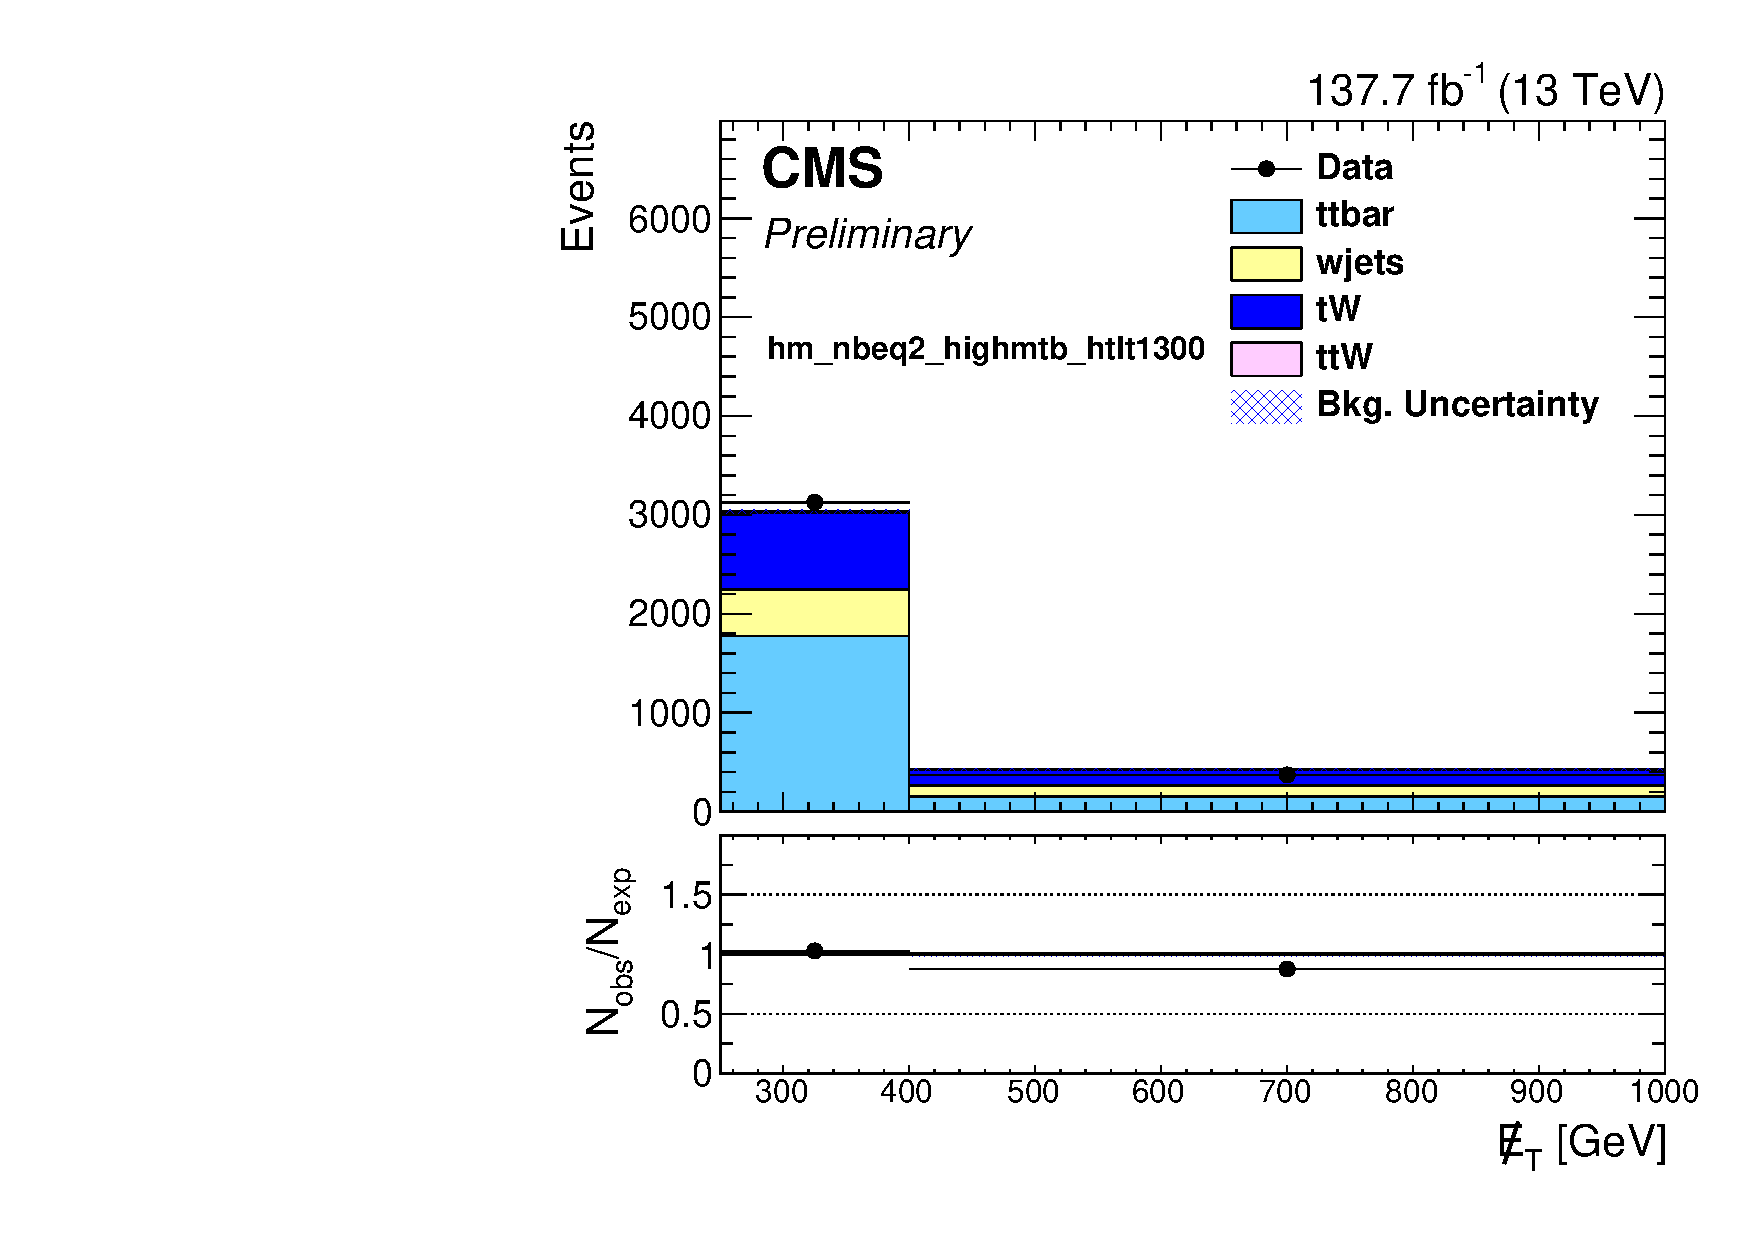
\includegraphics[width=0.32\textwidth]{../Research/SUSY/2019/LLB/lepcr_allEras/MET_pt_DataMC_hm_nbeq2_highmtb_nrtntnwgeq3_htlt1300__.pdf} 
  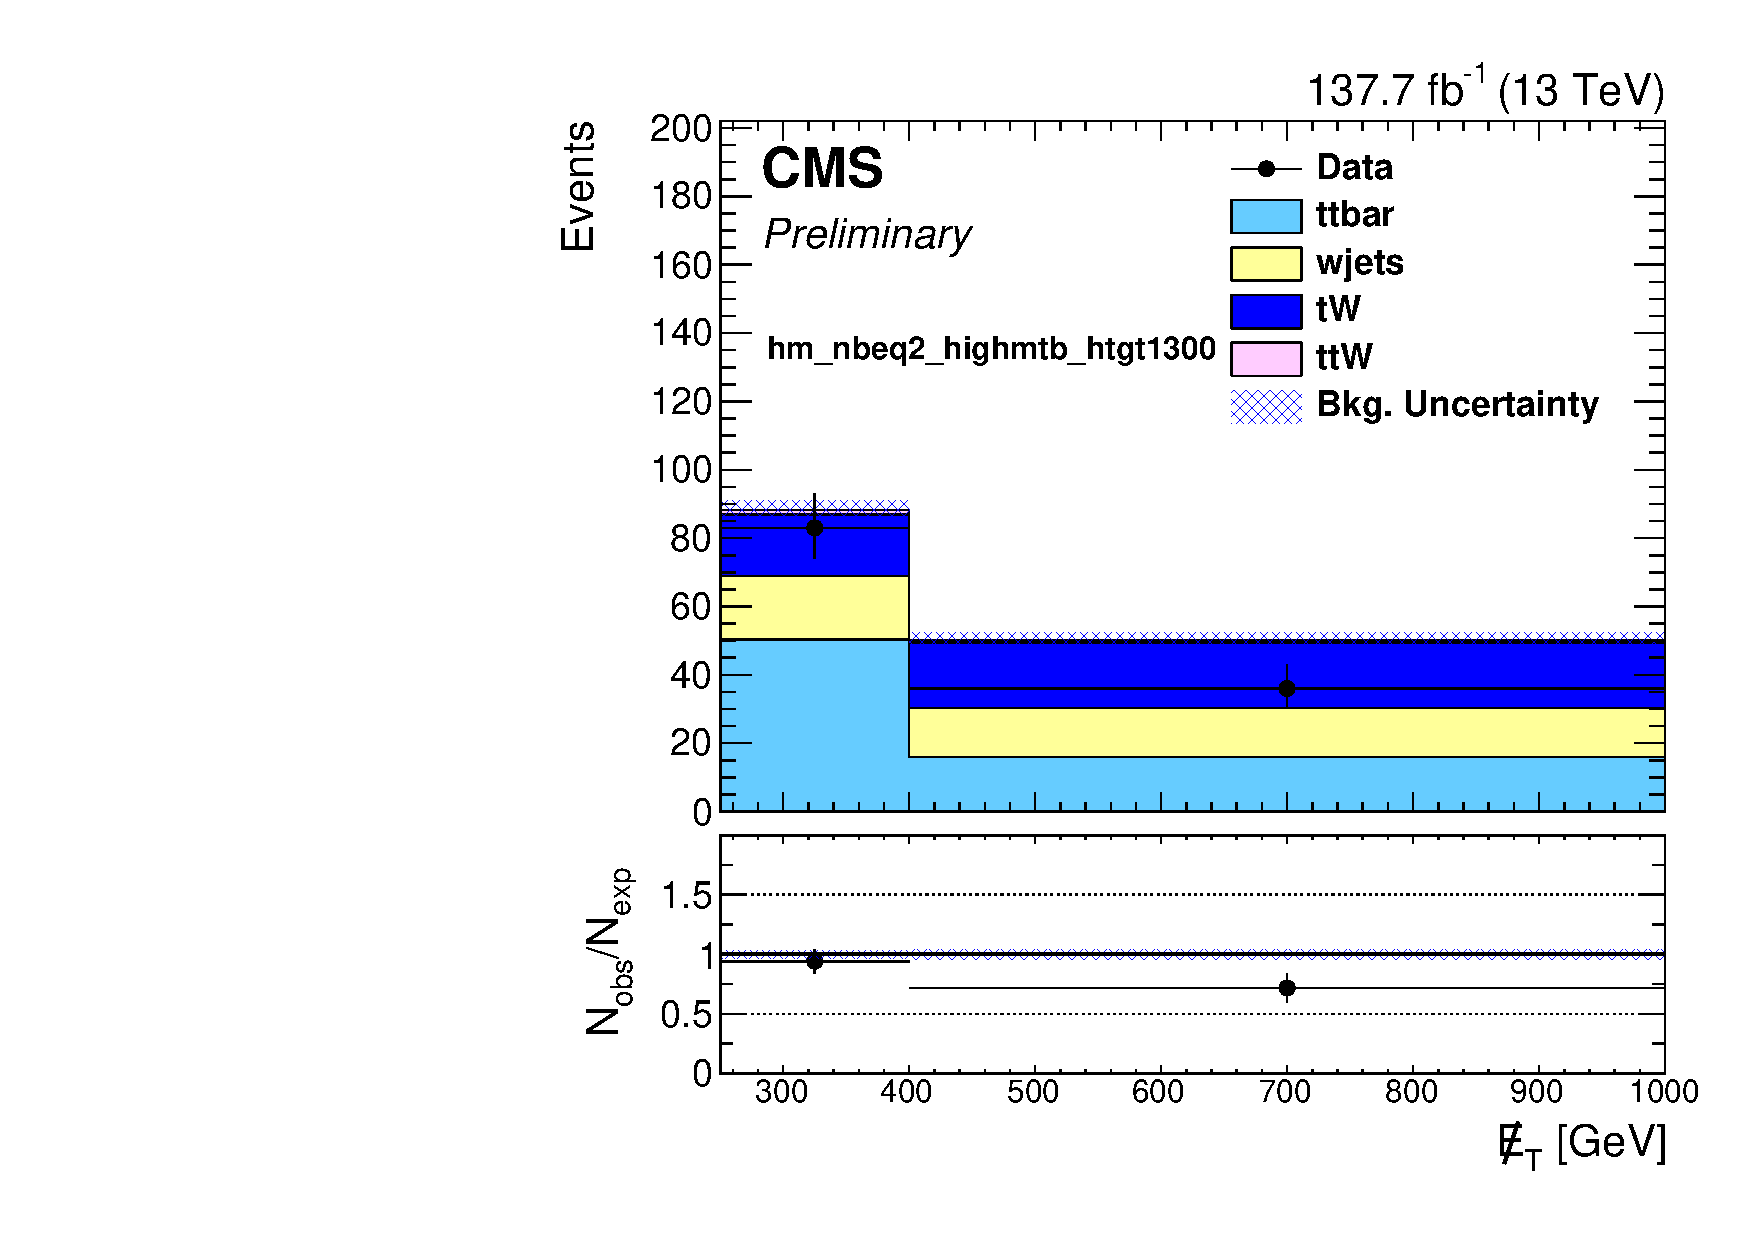
\includegraphics[width=0.32\textwidth]{../Research/SUSY/2019/LLB/lepcr_allEras/MET_pt_DataMC_hm_nbeq2_highmtb_nrtntnwgeq3_htgt1300__.pdf} \\
	\end{center}
	\caption{Comparison of the \met~distribution in the single-lepton sample after applying the high \dm~baseline selection in the $\nb=2$ and $\nt=2, \nrt=2,$ or $\nw=2$ region. Data and simulation are represented by the black points and stacked histograms, respectively. The error bars on the ratio of observed data to simulation correspo    nd to the data statistical uncertainty and the shaded blue band represents the statistical uncertainty on the simulation. These regions are included with the search regions in the simultaneous fit for the signal extraction in order to estimate the LL contribution.
	 %               The plots in the top row are for events with $\mtb<175$~\GeV, with $5\leq\nj<7$ on the left and $\nj\geq7$ on the right. 
	 %               The plots in the middle row are for events with $\mtb>175$~\GeV and $\nt=0, \nw=0$, with $5\leq\nj<7$ on the left and $\nj\geq7$ on the right. 
	 %               The plot in the bottom row is for events with $\mtb>175$~\GeV and $\nj\geq5$, with $\nt=0, \nw\geq1$ on the left, $\nt\geq1, \nw=0$ on the middle, and $\nt\geq1$, and $\nw\geq1$ on the right.
	 }
	\label{fig:llb-1lcr-datavsmc-hm-nb2-2}
\end{figure}

\begin{figure}[!htb]
	\begin{center}
  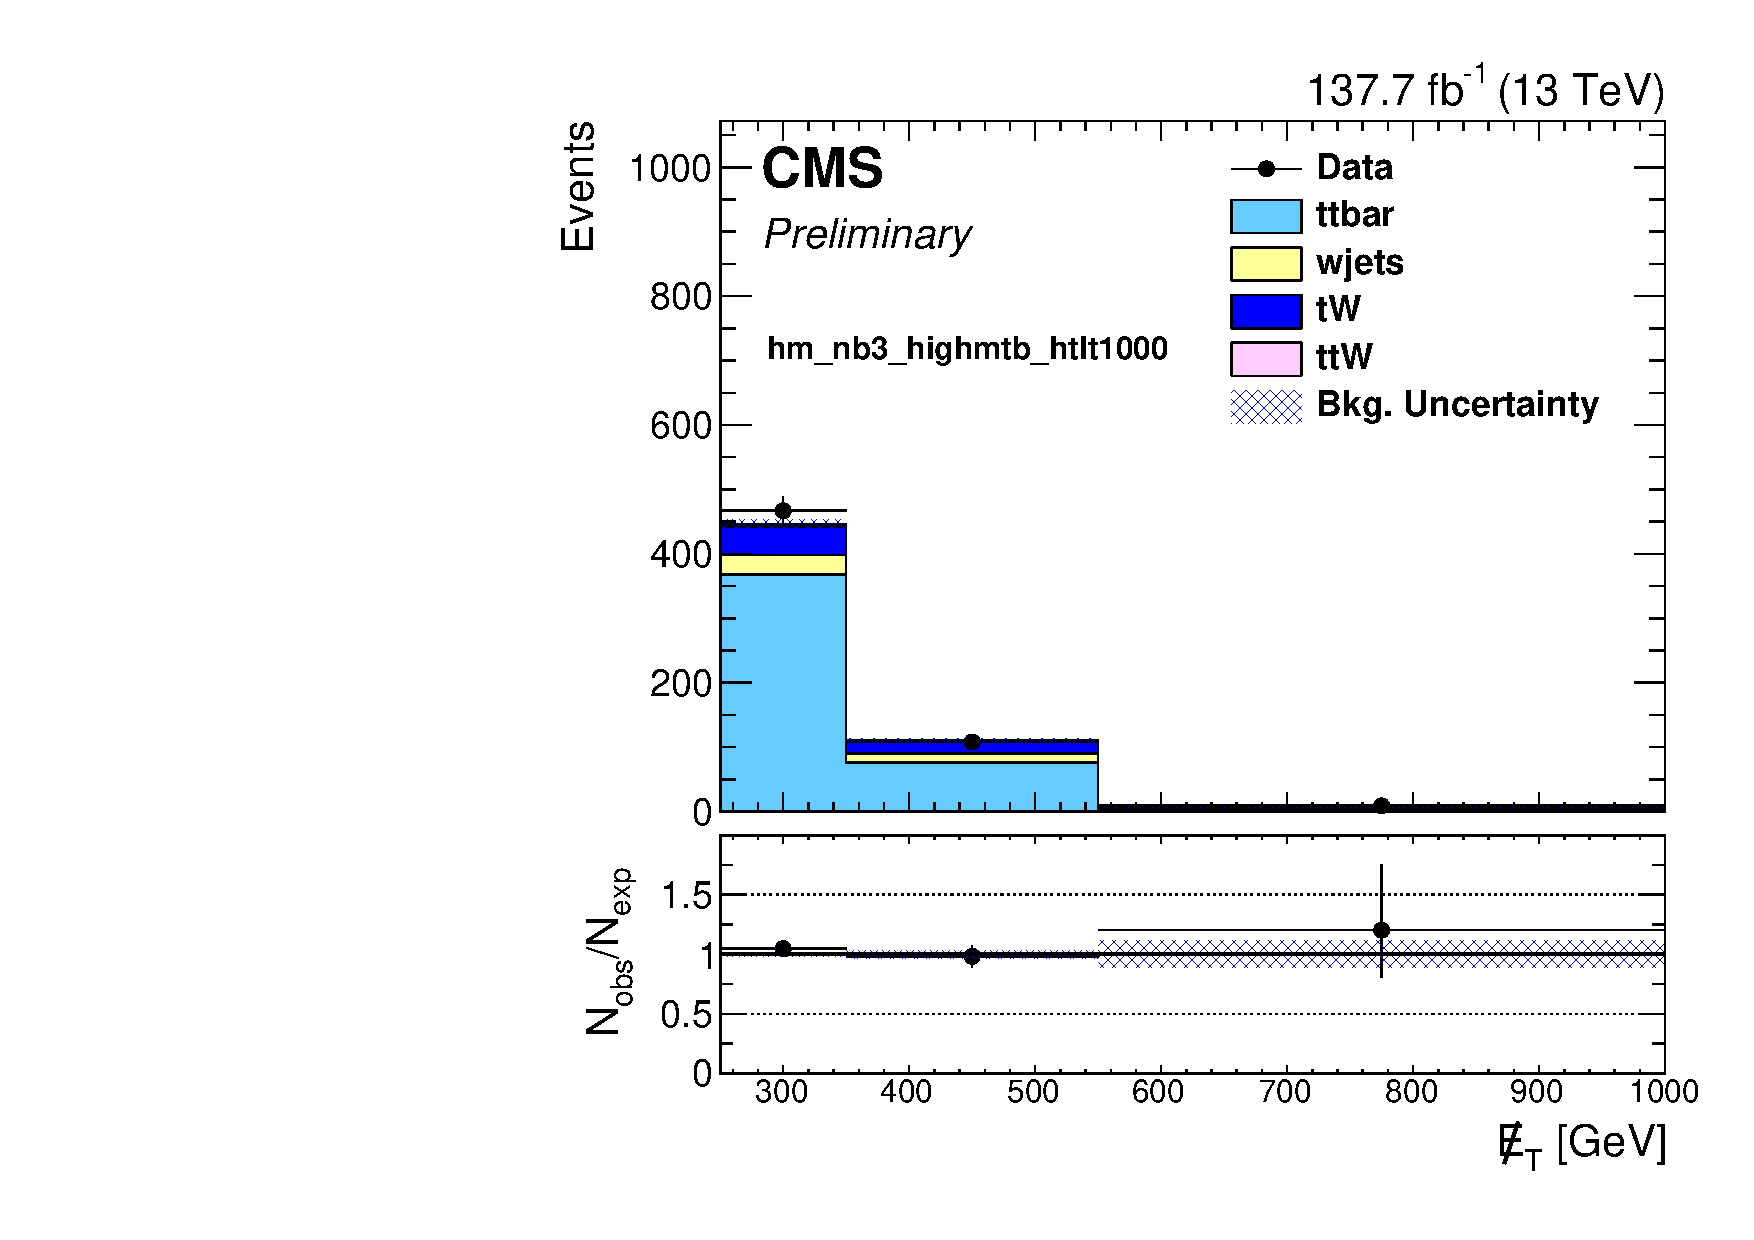
\includegraphics[width=0.32\textwidth]{../Research/SUSY/2019/LLB/lepcr_allEras/MET_pt_DataMC_hm_nb3_highmtb_nt1_nrt0_nw0_htlt1000__.pdf}
  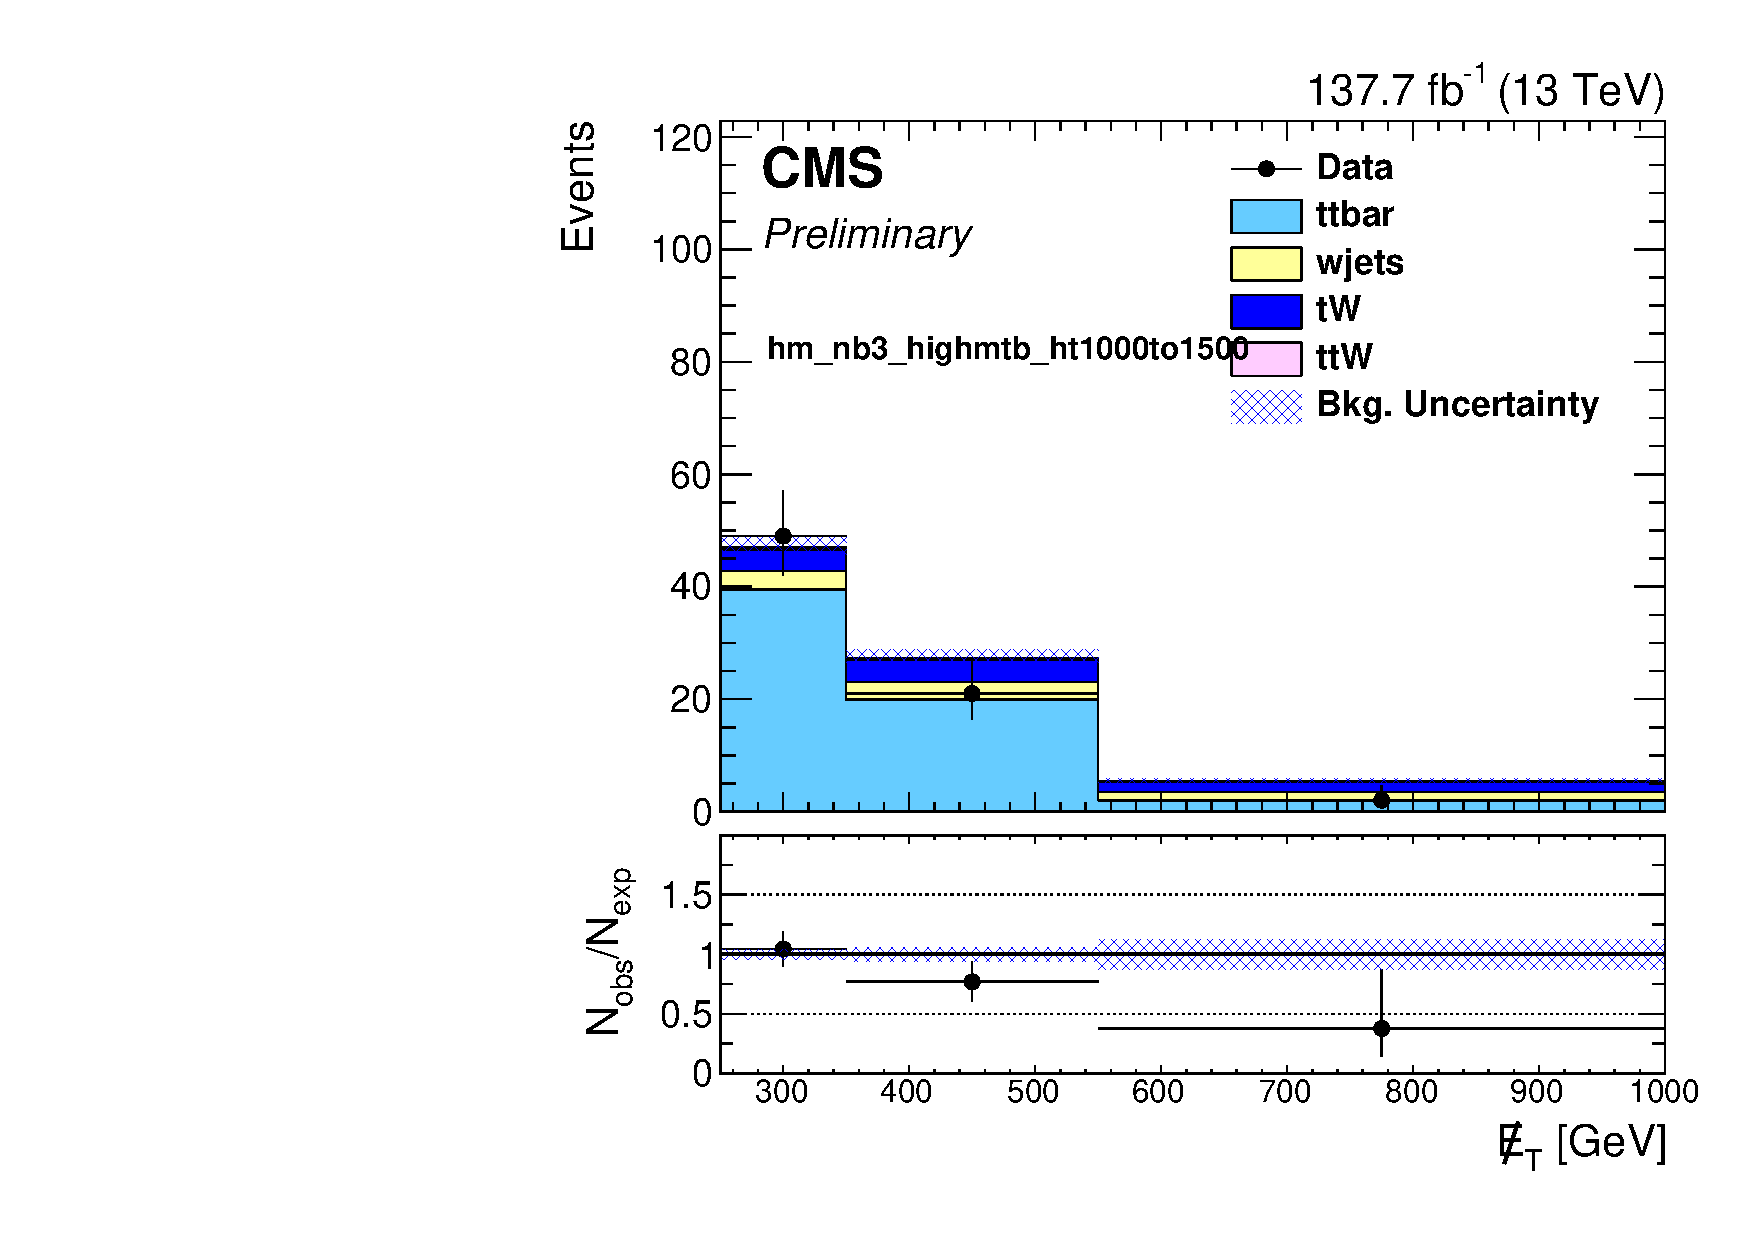
\includegraphics[width=0.32\textwidth]{../Research/SUSY/2019/LLB/lepcr_allEras/MET_pt_DataMC_hm_nb3_highmtb_nt1_nrt0_nw0_ht1000to1500__.pdf} 
  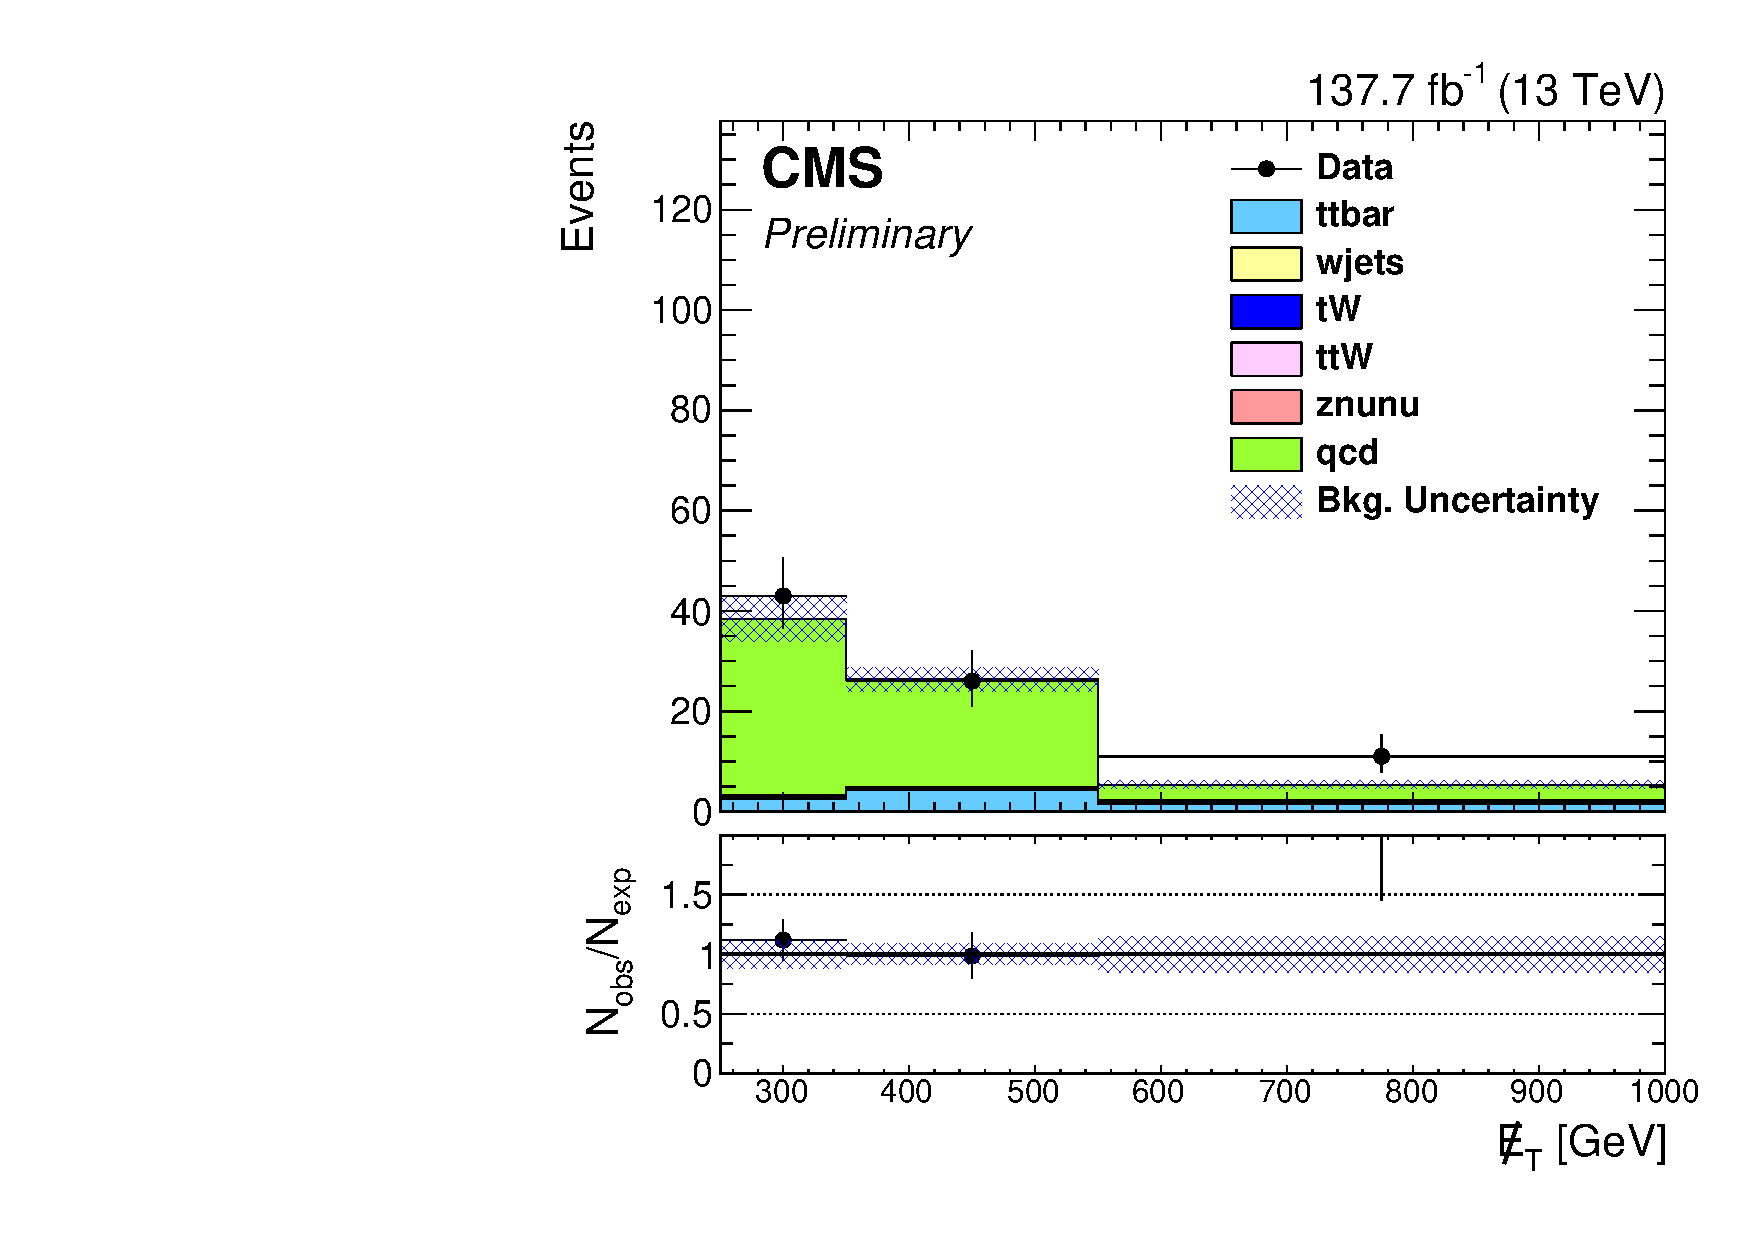
\includegraphics[width=0.32\textwidth]{../Research/SUSY/2019/LLB/lepcr_allEras/MET_pt_DataMC_hm_nb3_highmtb_nt1_nrt0_nw0_htgt1500__.pdf} \\
  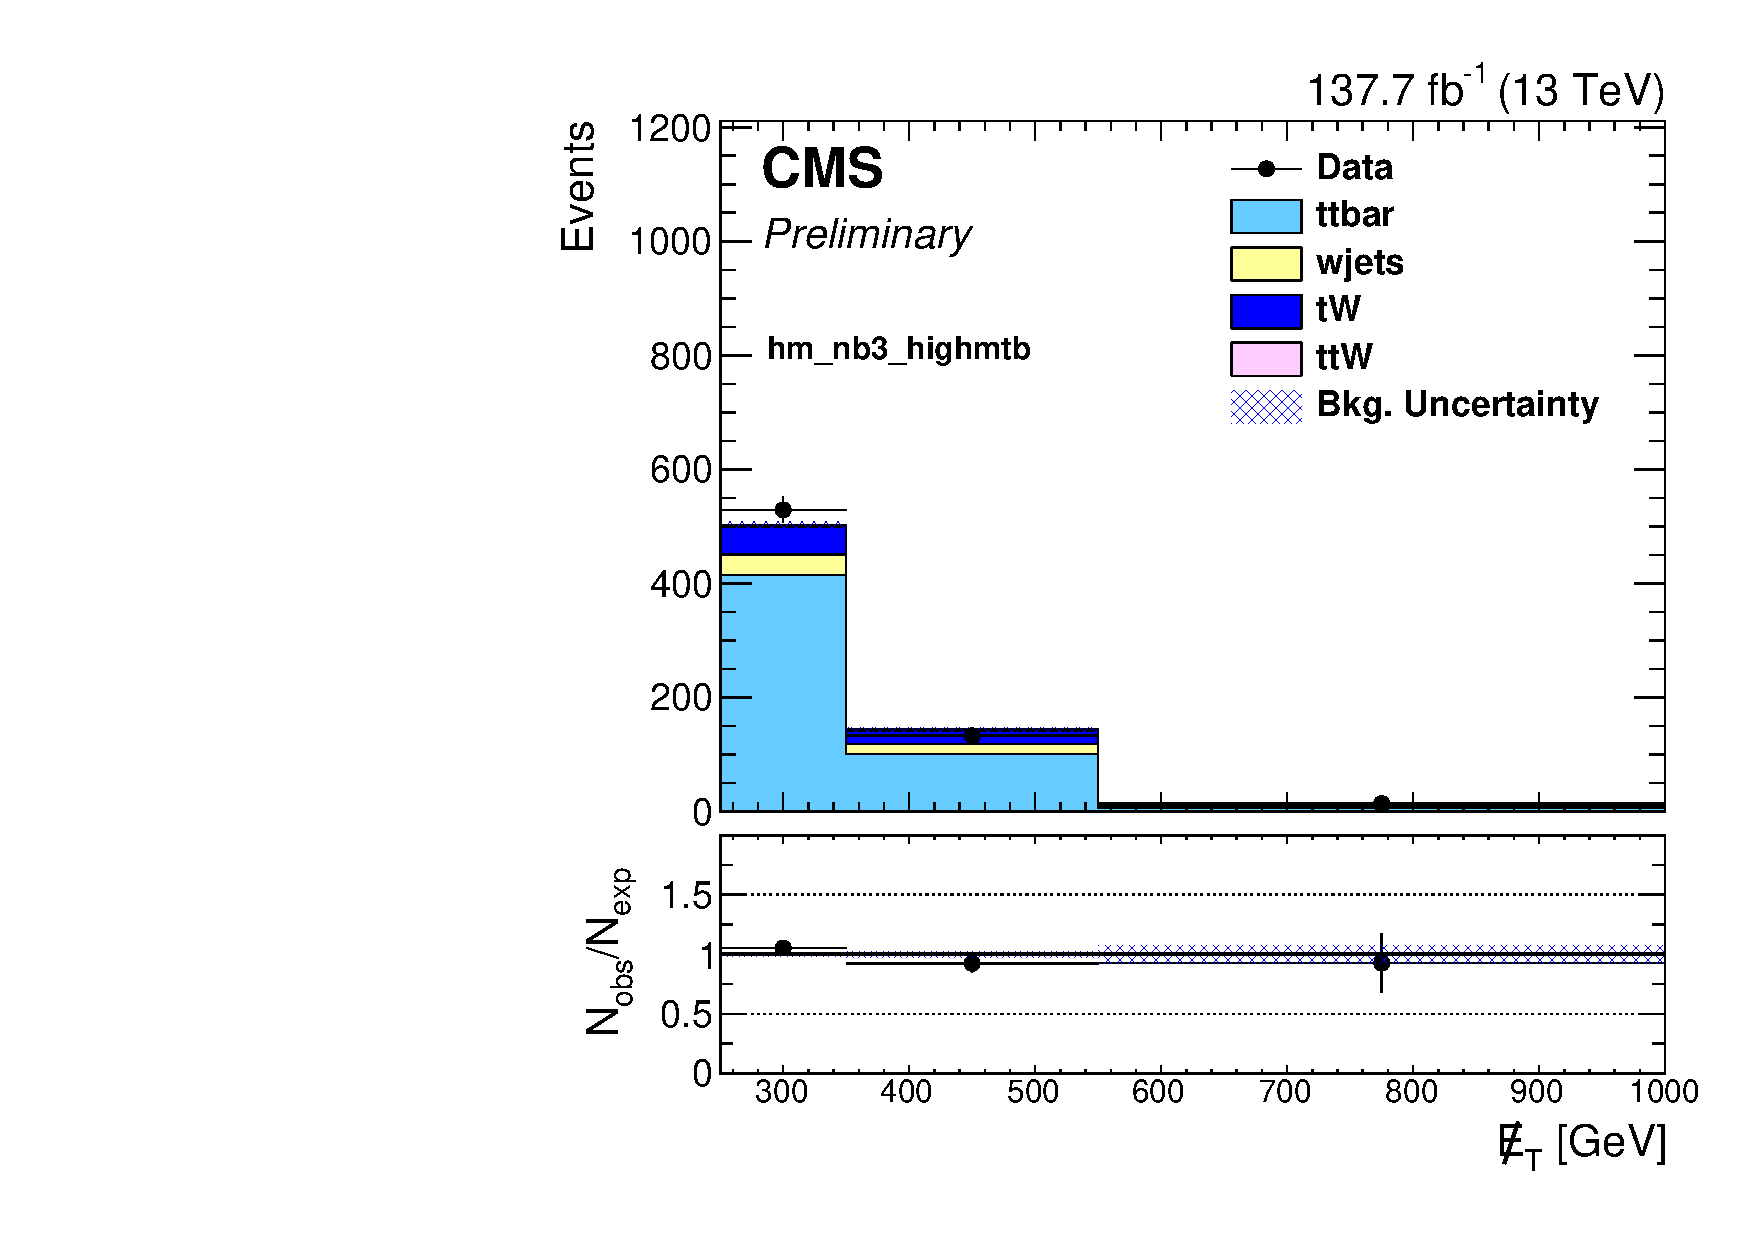
\includegraphics[width=0.32\textwidth]{../Research/SUSY/2019/LLB/lepcr_allEras/MET_pt_DataMC_hm_nb3_highmtb_nt0_nrt0_nw1__.pdf} 
  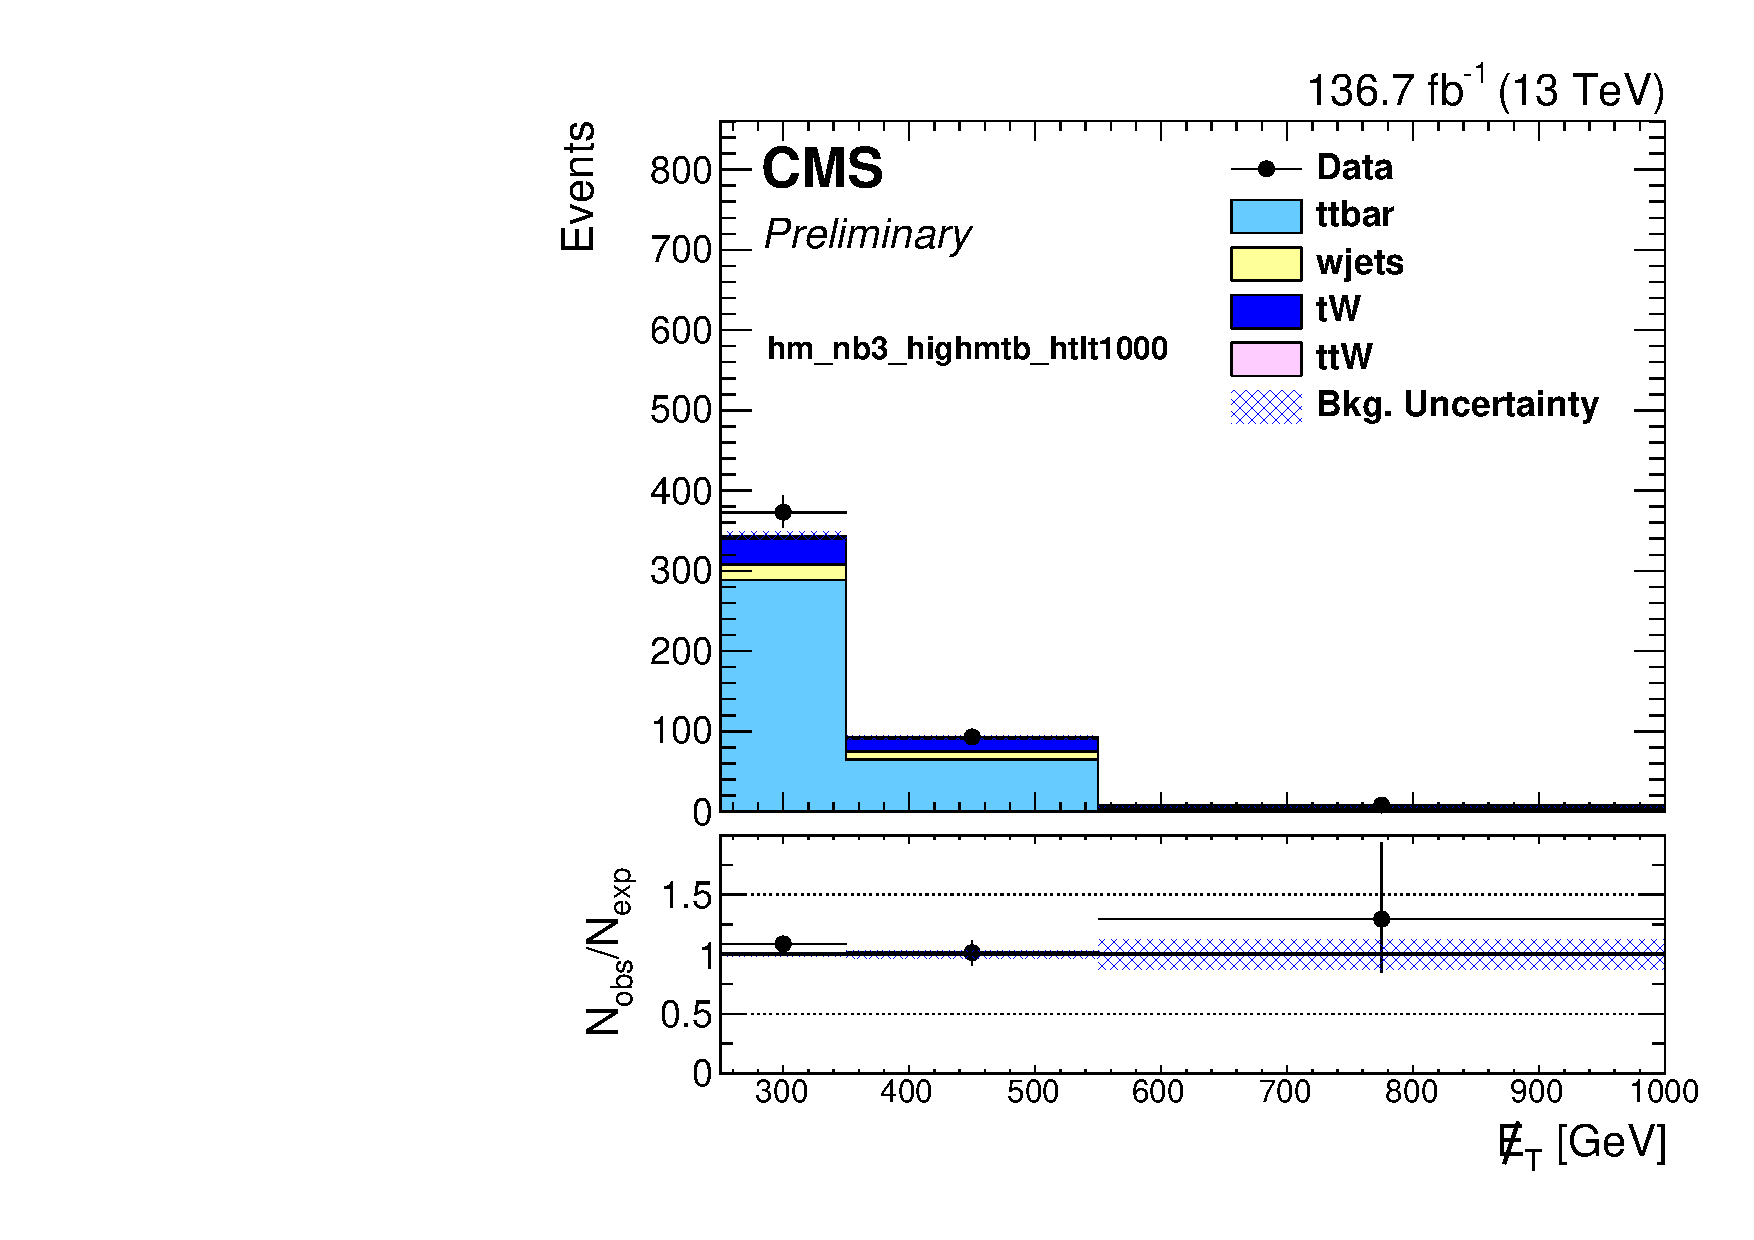
\includegraphics[width=0.32\textwidth]{../Research/SUSY/2019/LLB/lepcr_allEras/MET_pt_DataMC_hm_nb3_highmtb_nt0_nrt1_nw0_htlt1000__.pdf} \\
  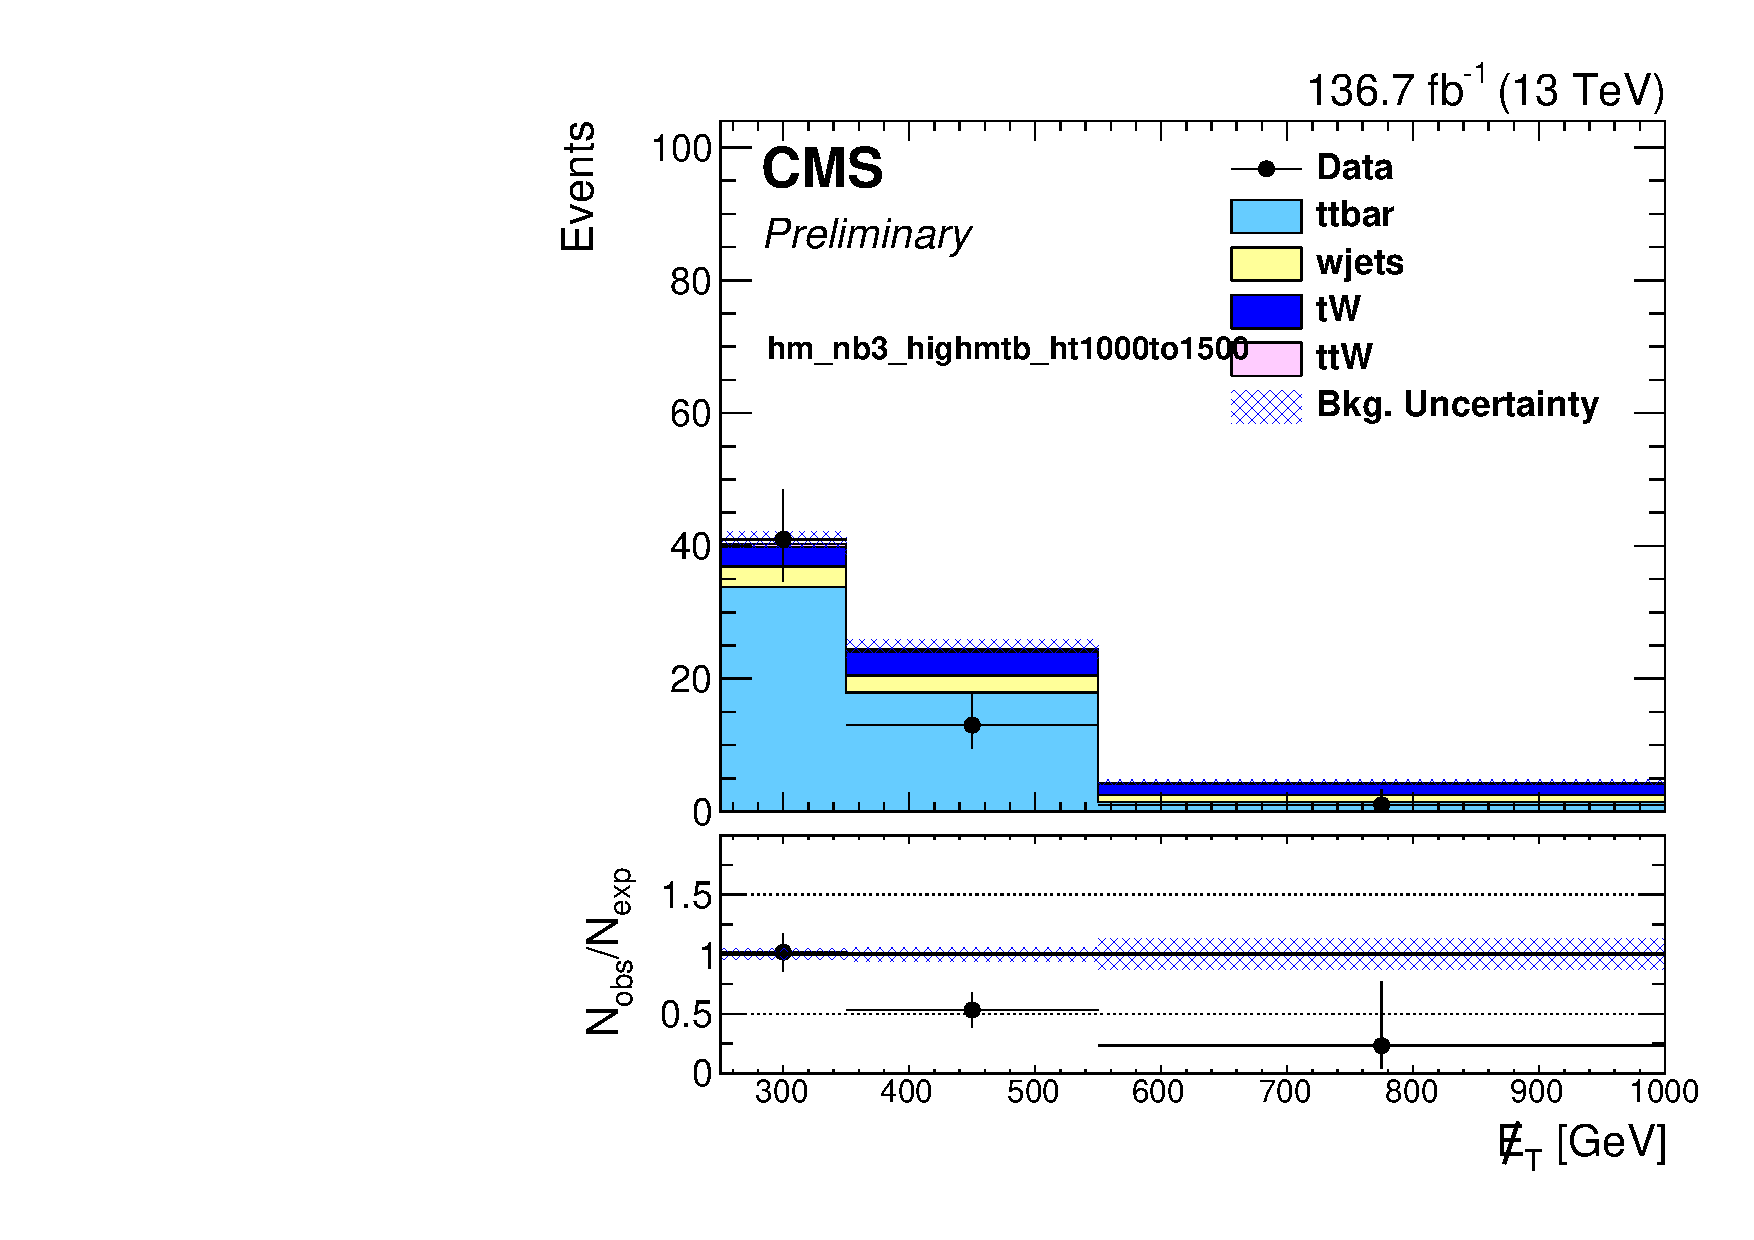
\includegraphics[width=0.32\textwidth]{../Research/SUSY/2019/LLB/lepcr_allEras/MET_pt_DataMC_hm_nb3_highmtb_nt0_nrt1_nw0_ht1000to1500__.pdf}  
  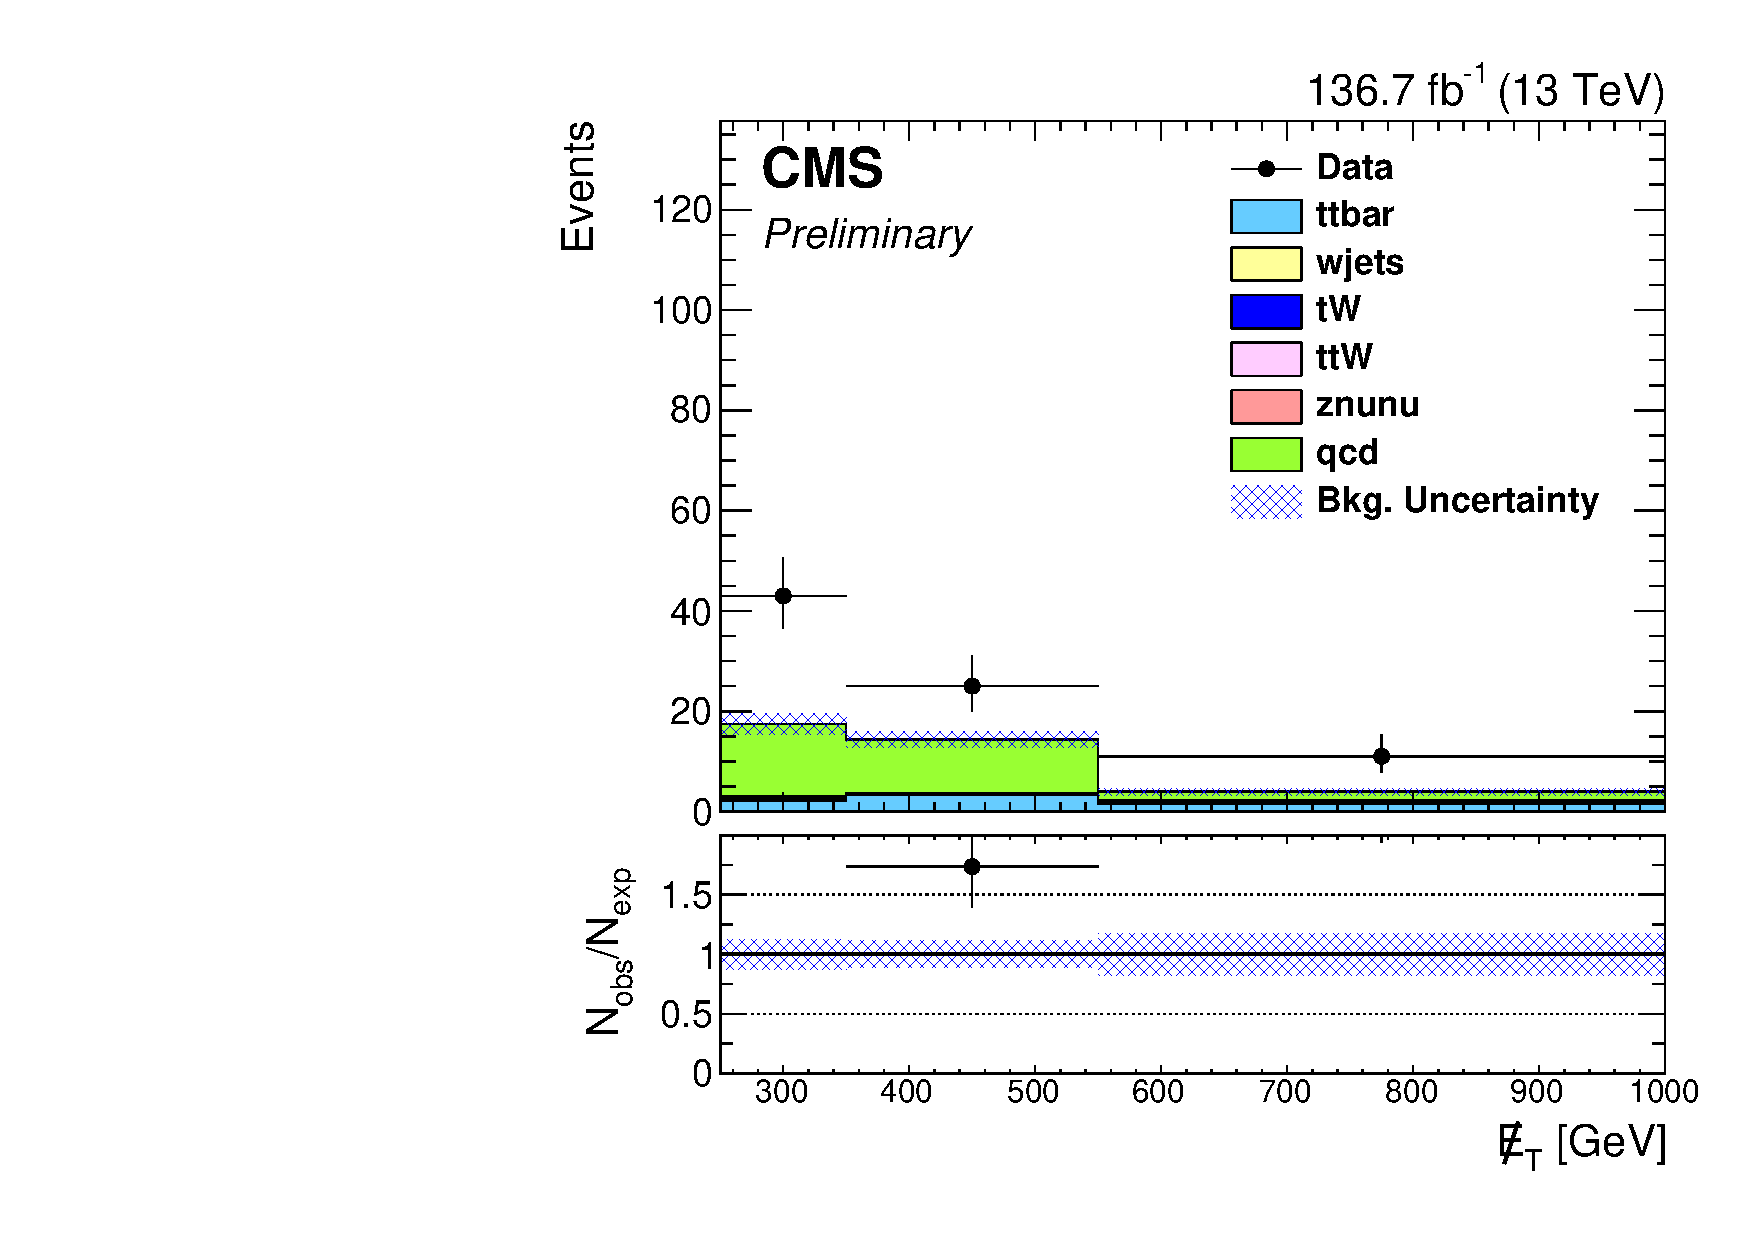
\includegraphics[width=0.32\textwidth]{../Research/SUSY/2019/LLB/lepcr_allEras/MET_pt_DataMC_hm_nb3_highmtb_nt0_nrt1_nw0_htgt1500__.pdf} \\
  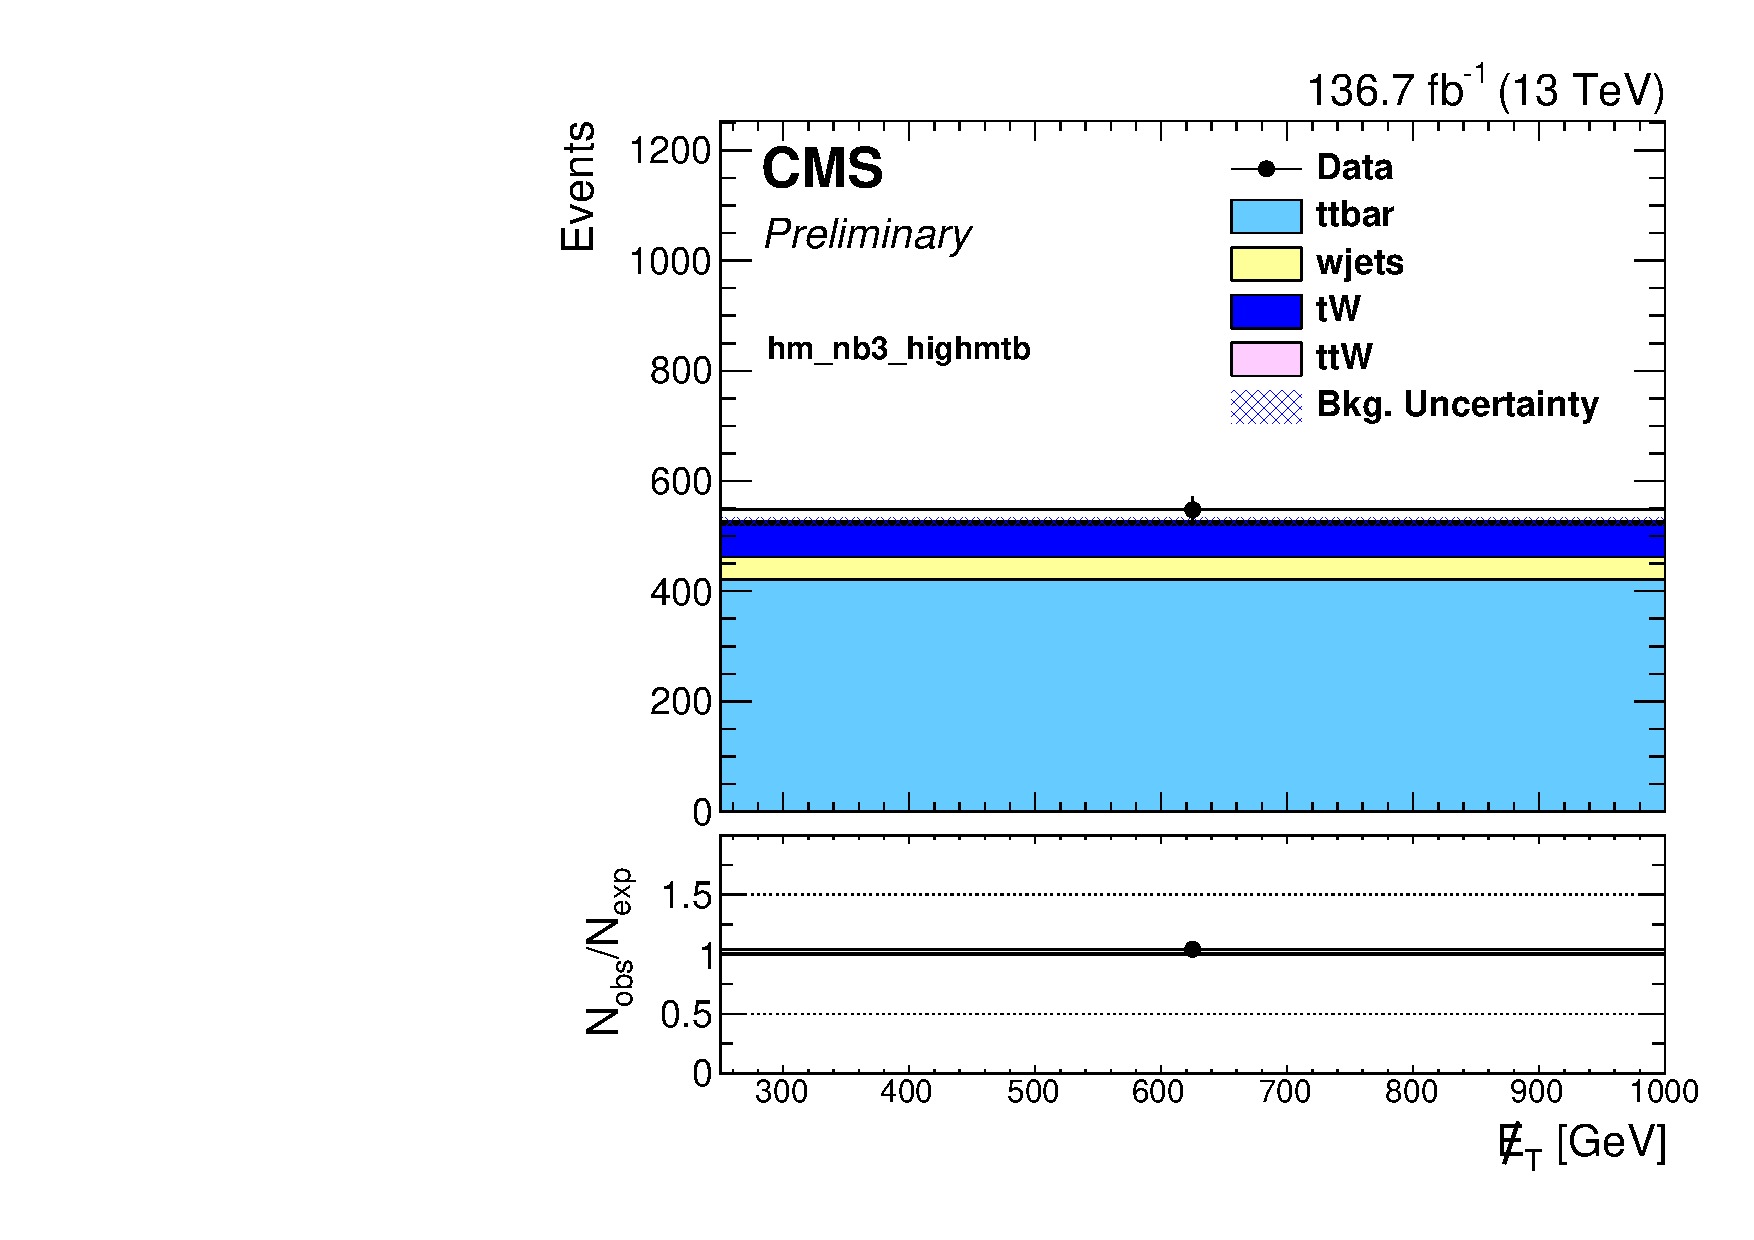
\includegraphics[width=0.32\textwidth]{../Research/SUSY/2019/LLB/lepcr_allEras/MET_pt_DataMC_hm_nb3_highmtb_nt1_nrt0_nw1__.pdf} 
  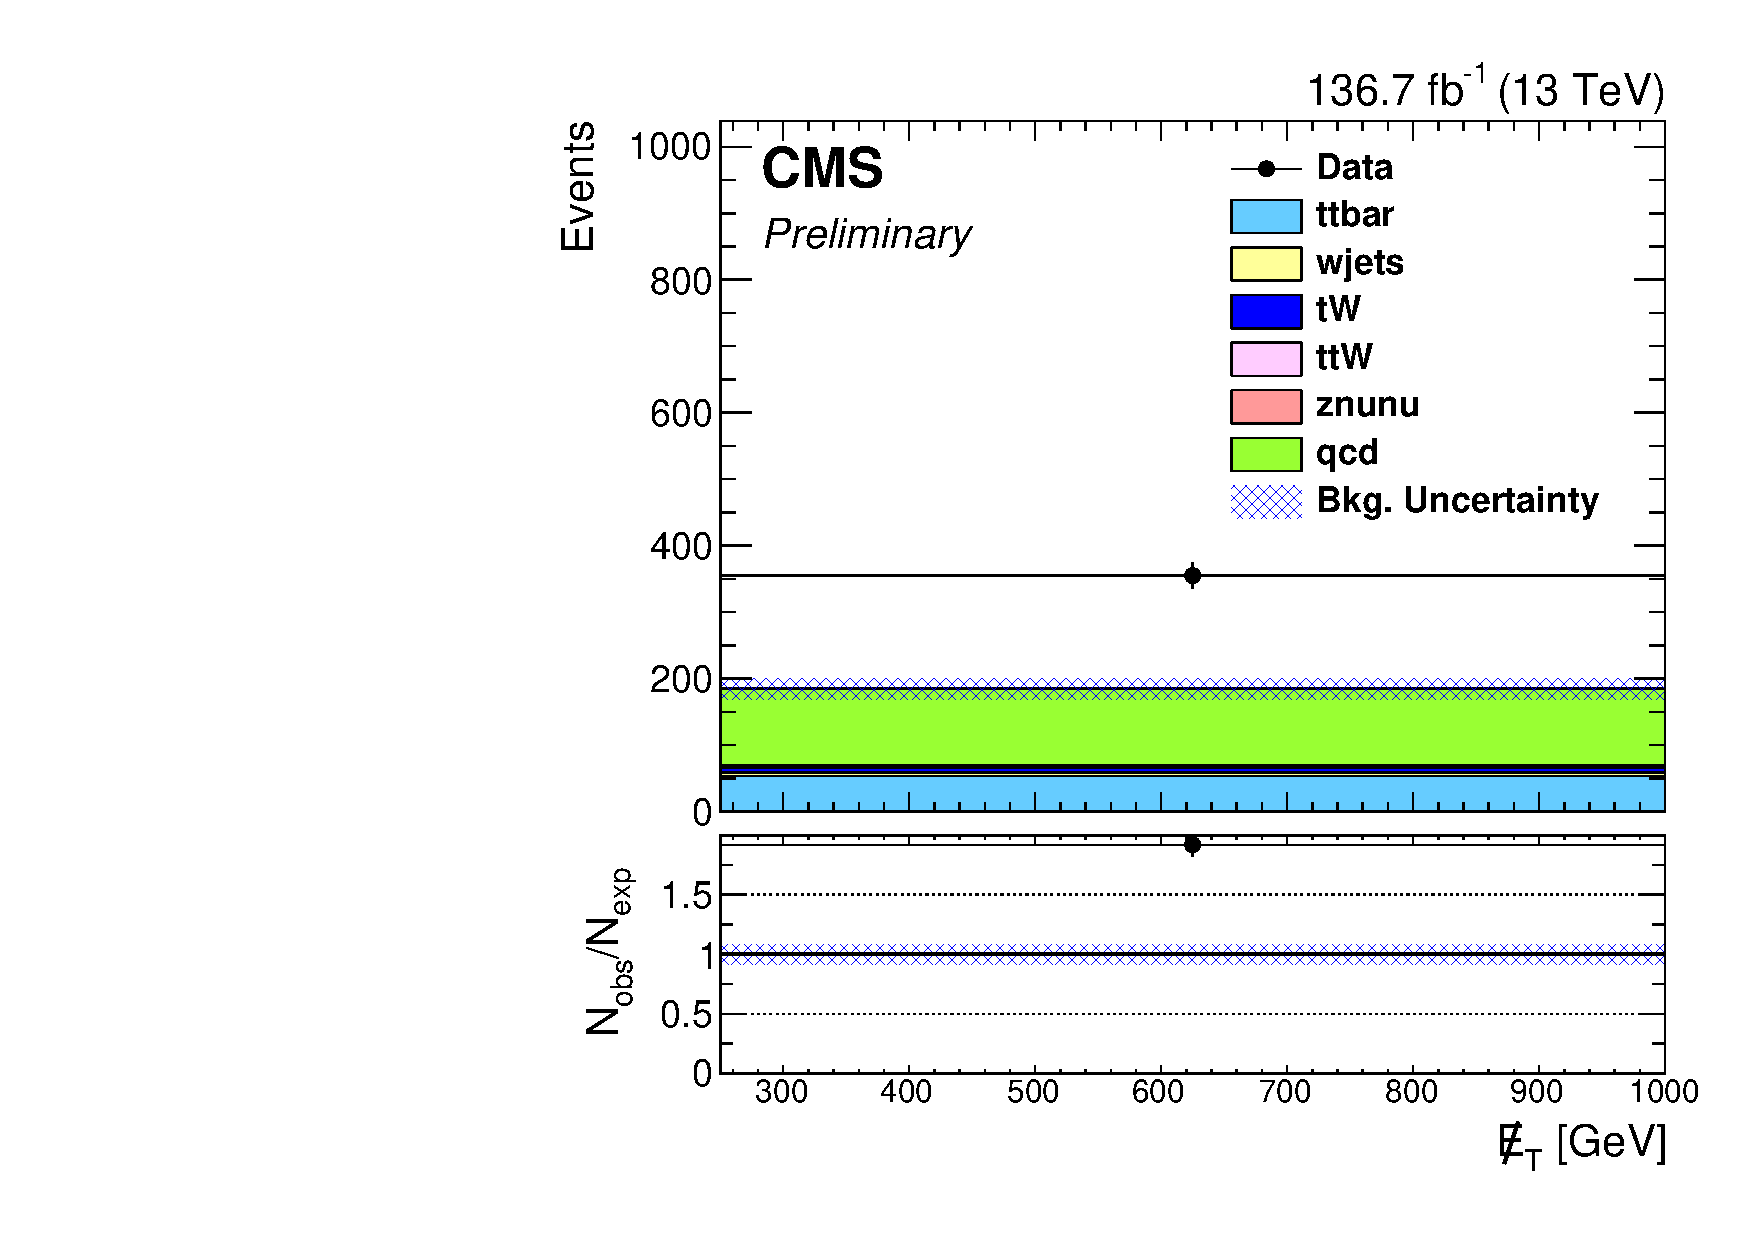
\includegraphics[width=0.32\textwidth]{../Research/SUSY/2019/LLB/lepcr_allEras/MET_pt_DataMC_hm_nb3_highmtb_nt0_nrt1_nw1__.pdf} \\
	\end{center}
	\caption{Comparison of the \met~distribution in the single-lepton sample after applying the high \dm~baseline selection in the $\nb\geq3$ and $\nt=1, \nrt=1,$ or $\nw=1$ region. Data and simulation are represented by the black points and stacked histograms, respectively. The error bars on the ratio of observed data to simulation correspo    nd to the data statistical uncertainty and the shaded blue band represents the statistical uncertainty on the simulation. These regions are included with the search regions in the simultaneous fit for the signal extraction in order to estimate the LL contribution.
	 %               The plots in the top row are for events with $\mtb<175$~\GeV, with $5\leq\nj<7$ on the left and $\nj\geq7$ on the right. 
	 %               The plots in the middle row are for events with $\mtb>175$~\GeV and $\nt=0, \nw=0$, with $5\leq\nj<7$ on the left and $\nj\geq7$ on the right. 
	 %               The plot in the bottom row is for events with $\mtb>175$~\GeV and $\nj\geq5$, with $\nt=0, \nw\geq1$ on the left, $\nt\geq1, \nw=0$ on the middle, and $\nt\geq1$, and $\nw\geq1$ on the right.
	 }
	\label{fig:llb-1lcr-datavsmc-hm-nb3-1}
\end{figure}

\begin{figure}[!htb]
	\begin{center}
  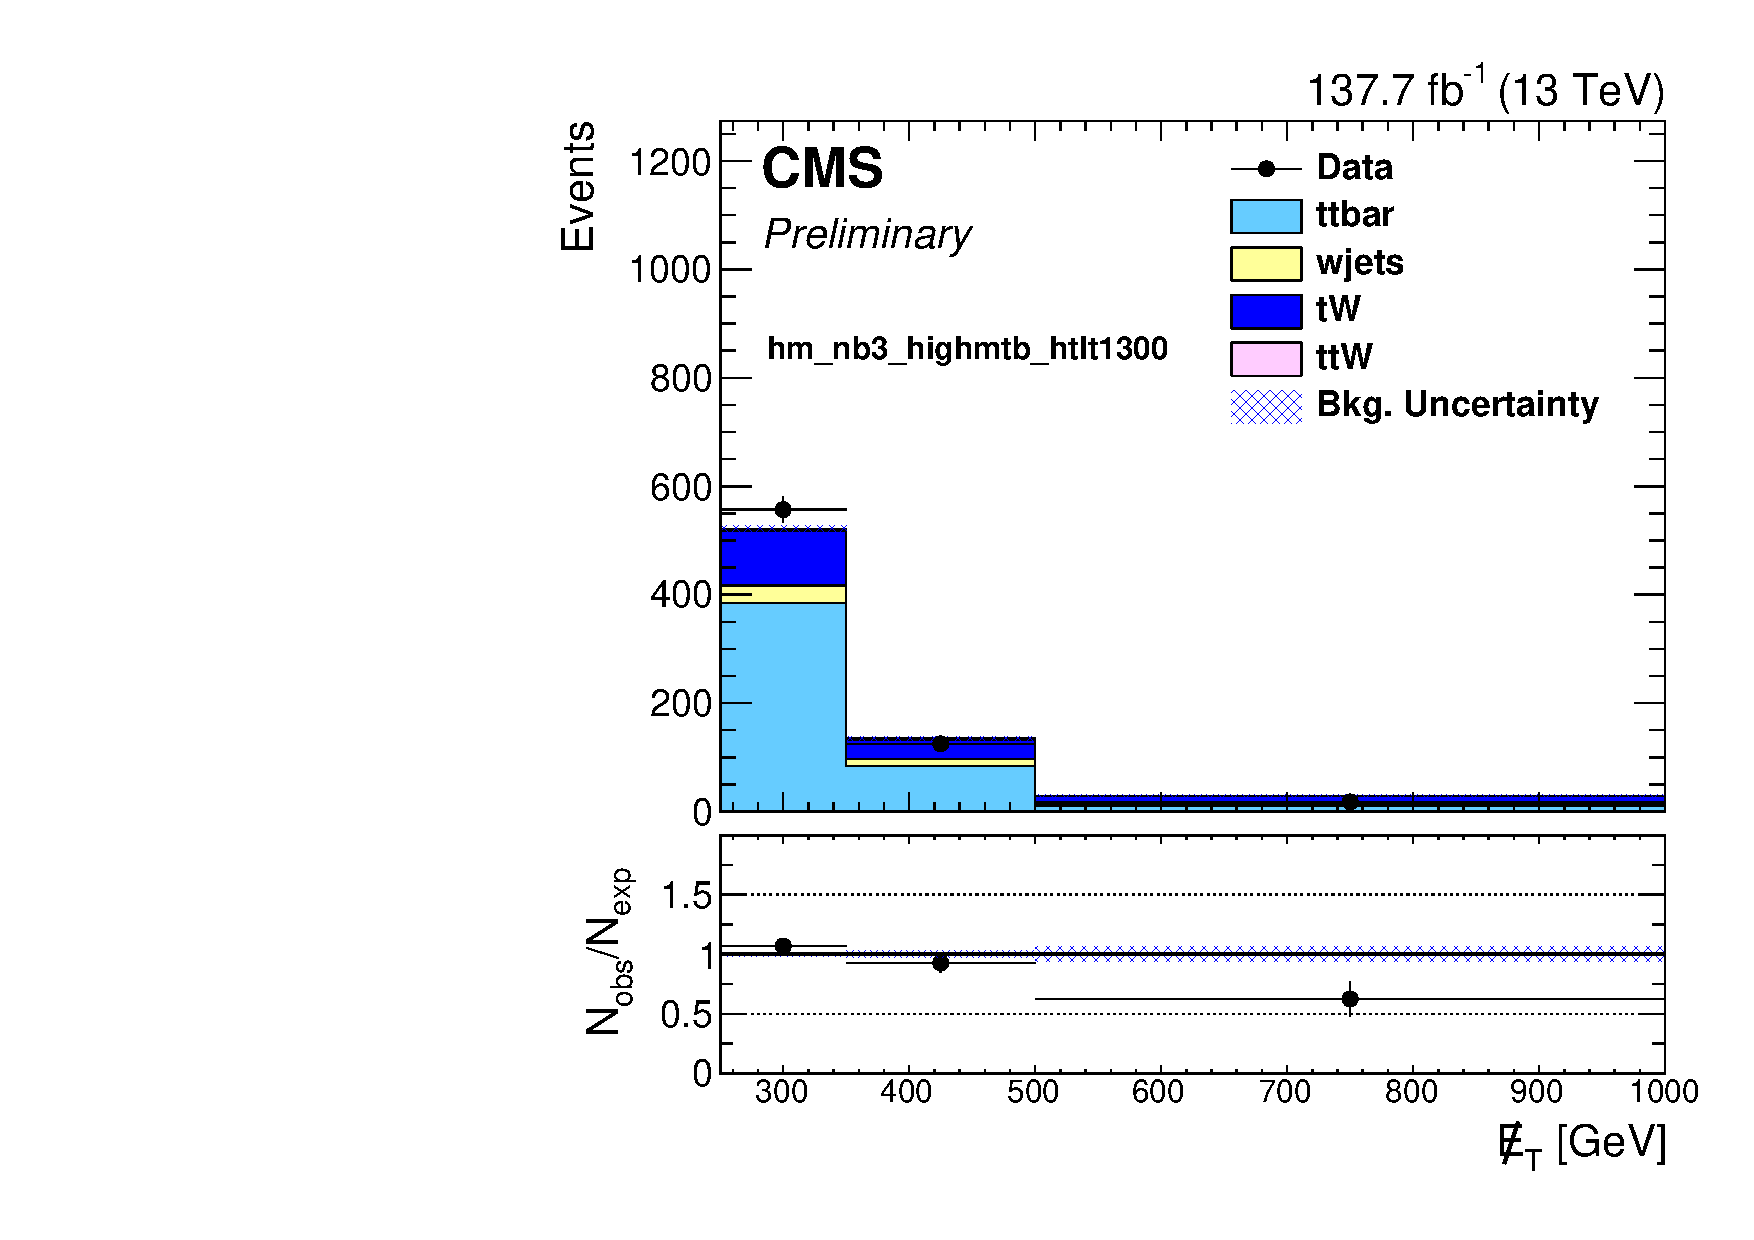
\includegraphics[width=0.32\textwidth]{../Research/SUSY/2019/LLB/lepcr_allEras/MET_pt_DataMC_hm_nb3_highmtb_nt1_nrt1_nw0_htlt1300__.pdf} 
  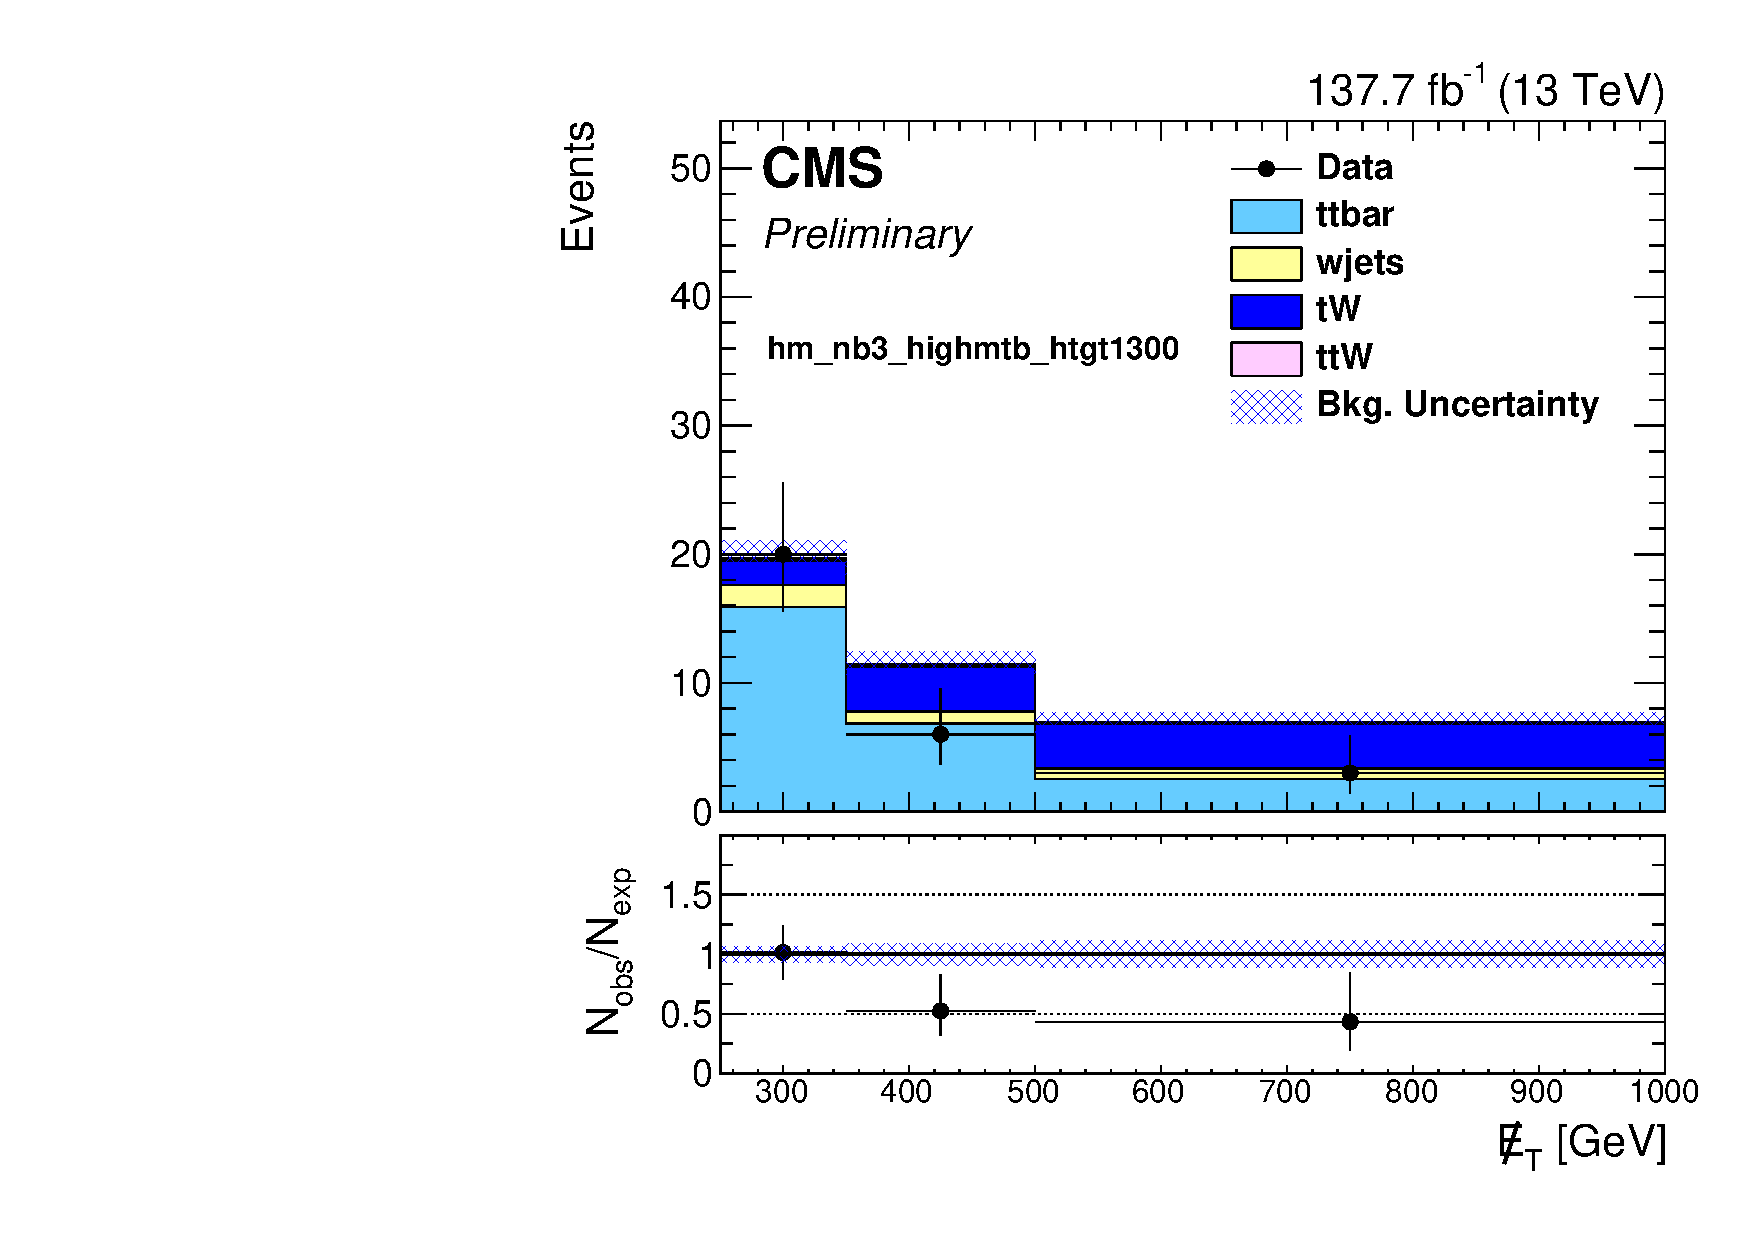
\includegraphics[width=0.32\textwidth]{../Research/SUSY/2019/LLB/lepcr_allEras/MET_pt_DataMC_hm_nb3_highmtb_nt1_nrt1_nw0_htgt1300__.pdf} \\  
  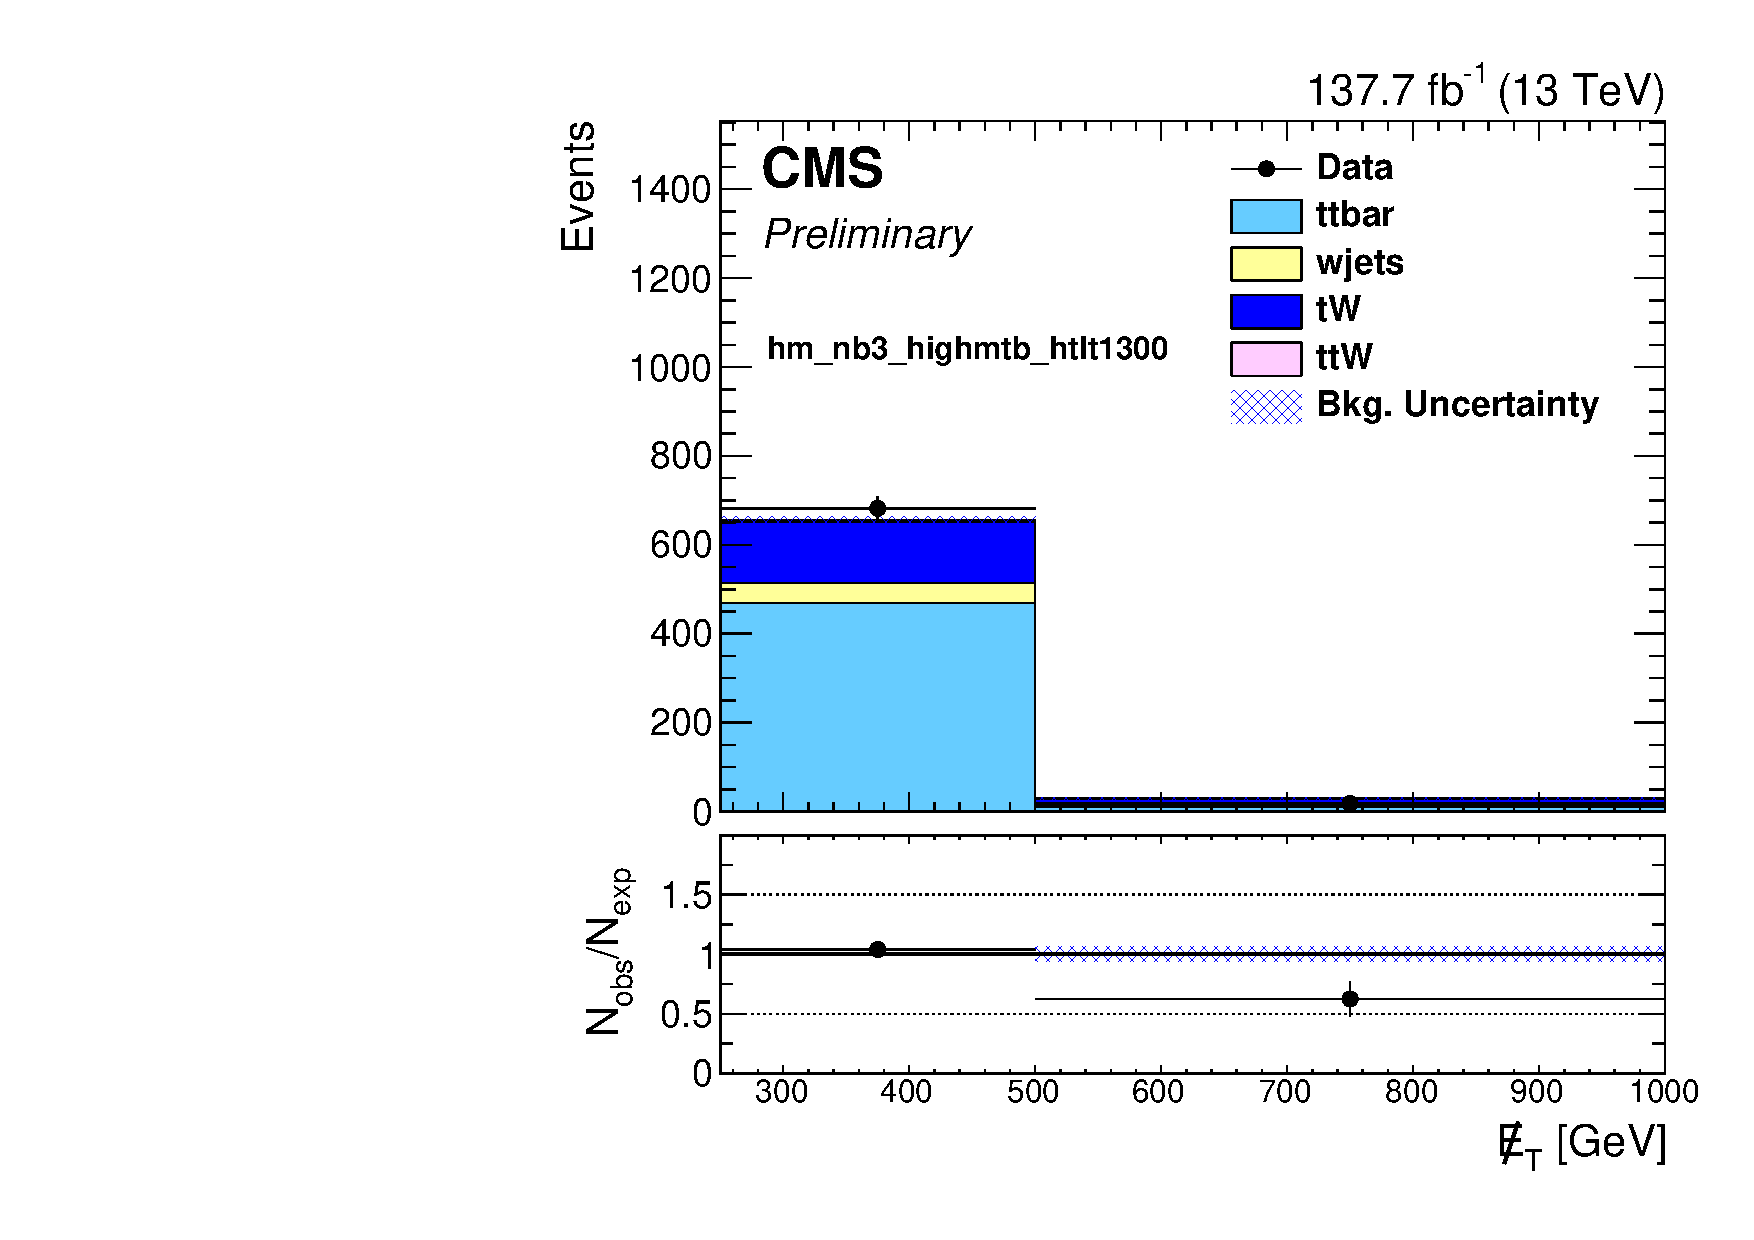
\includegraphics[width=0.32\textwidth]{../Research/SUSY/2019/LLB/lepcr_allEras/MET_pt_DataMC_hm_nb3_highmtb_nt2_nrt0_nw0_htlt1300__.pdf} 
  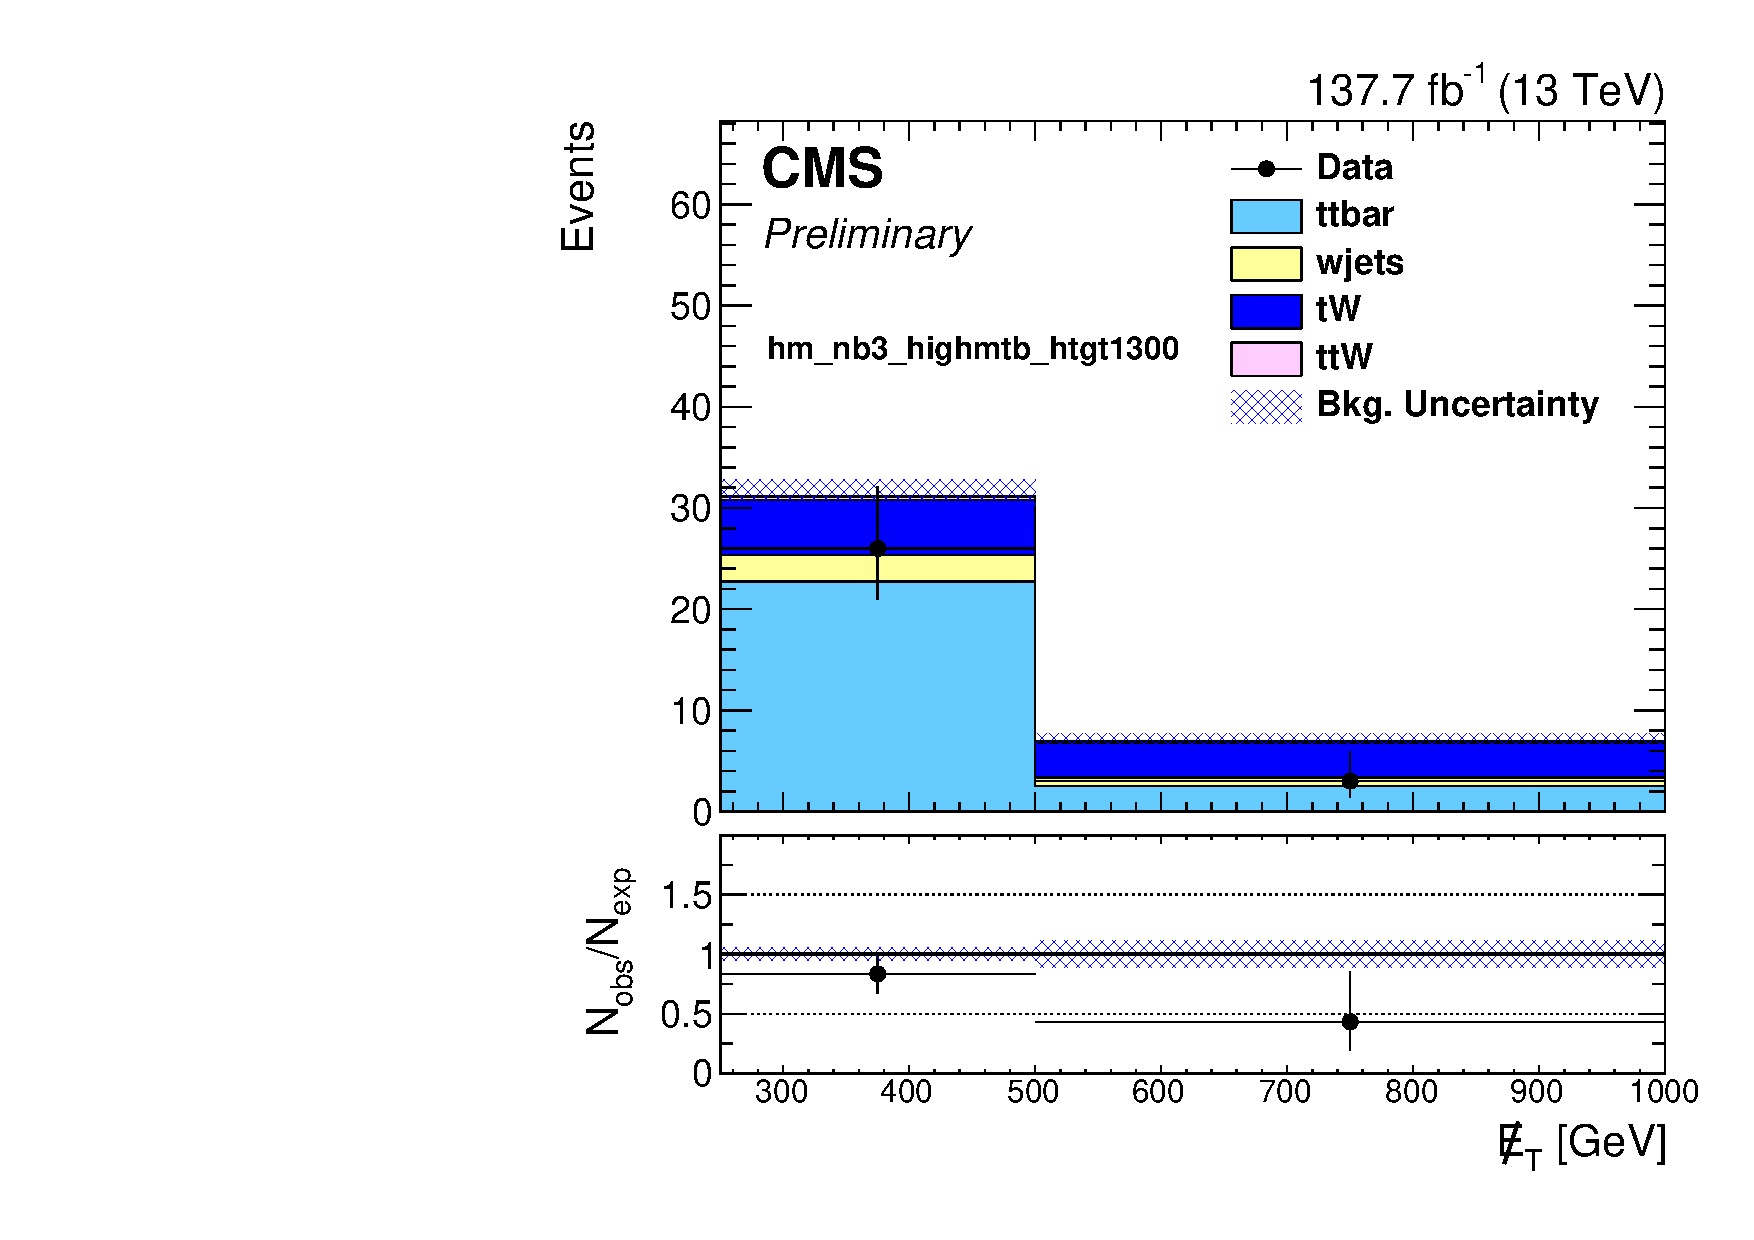
\includegraphics[width=0.32\textwidth]{../Research/SUSY/2019/LLB/lepcr_allEras/MET_pt_DataMC_hm_nb3_highmtb_nt2_nrt0_nw0_htgt1300__.pdf} 
  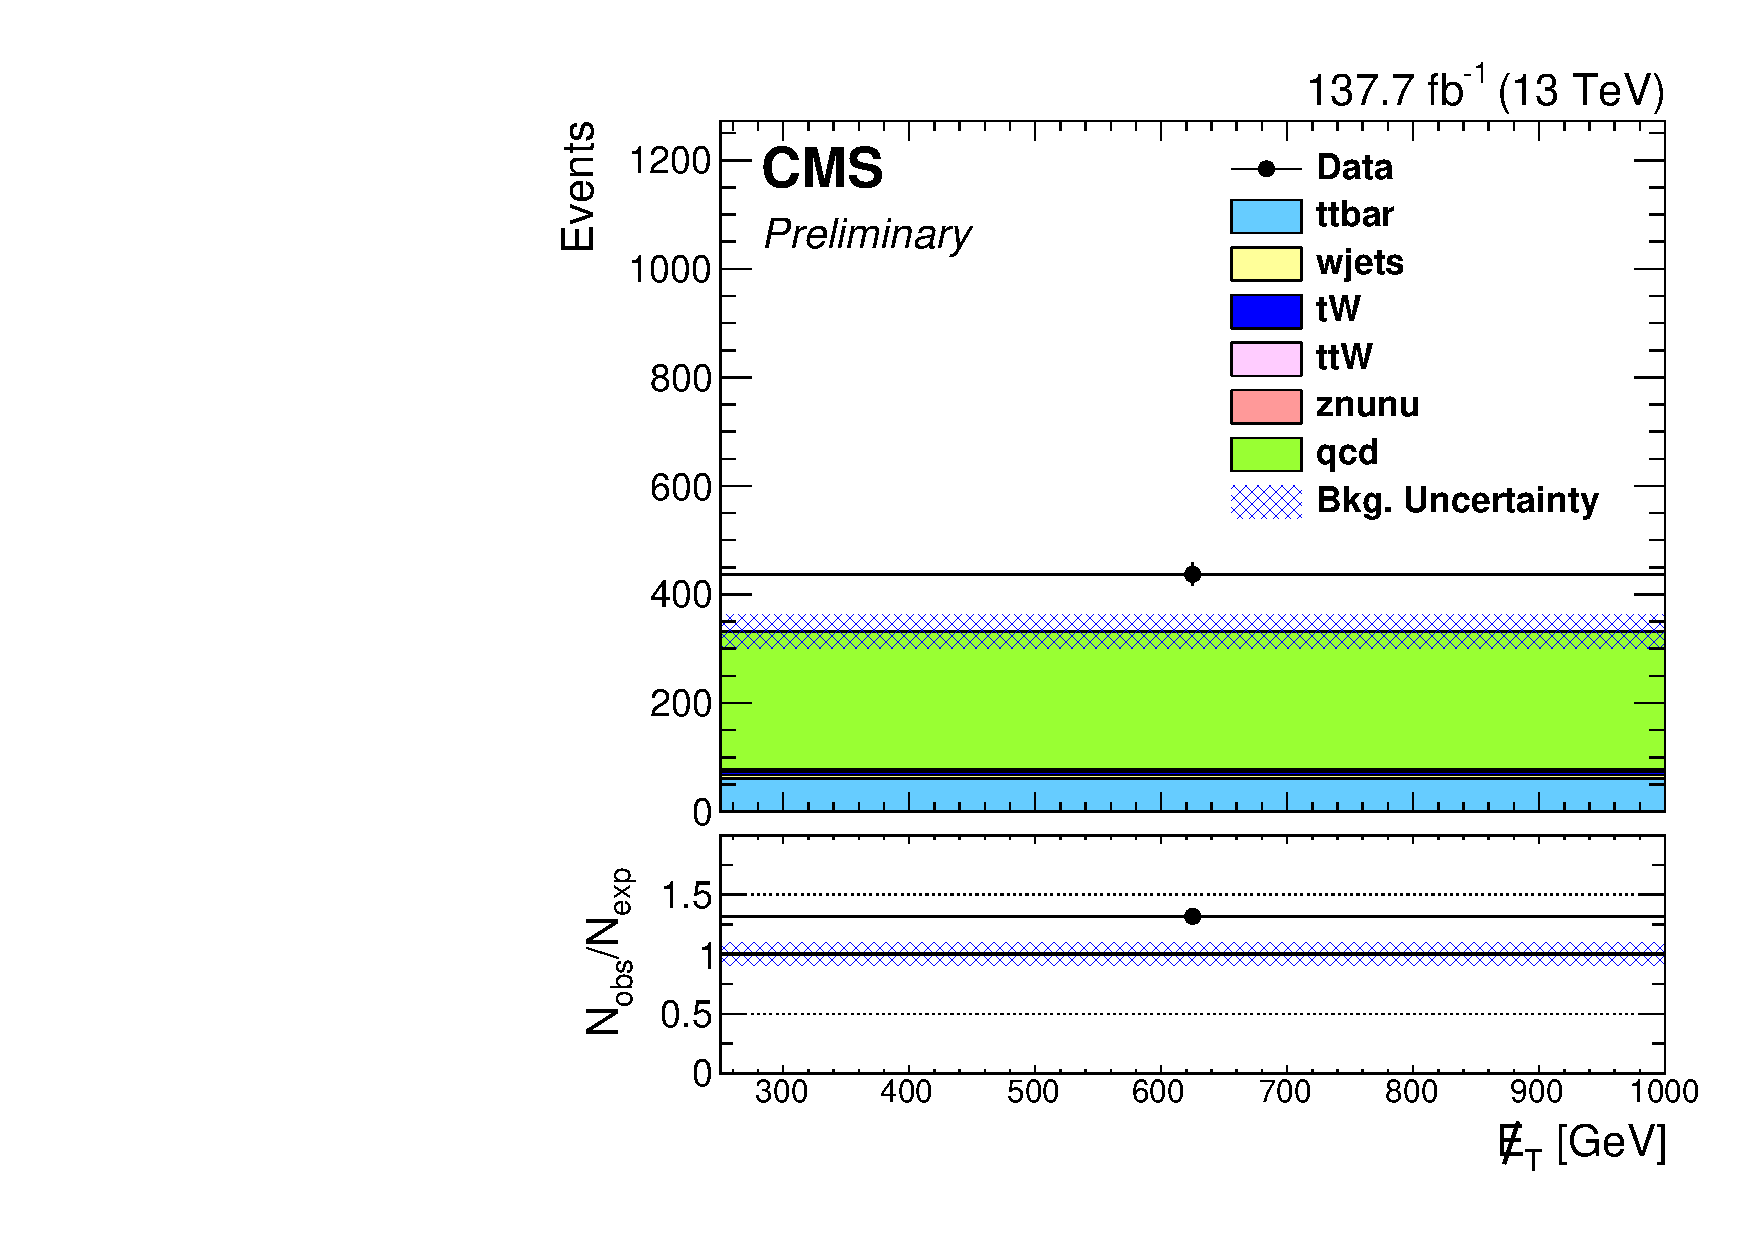
\includegraphics[width=0.32\textwidth]{../Research/SUSY/2019/LLB/lepcr_allEras/MET_pt_DataMC_hm_nb3_highmtb_nt0_nrt0_nw2__.pdf} \\
  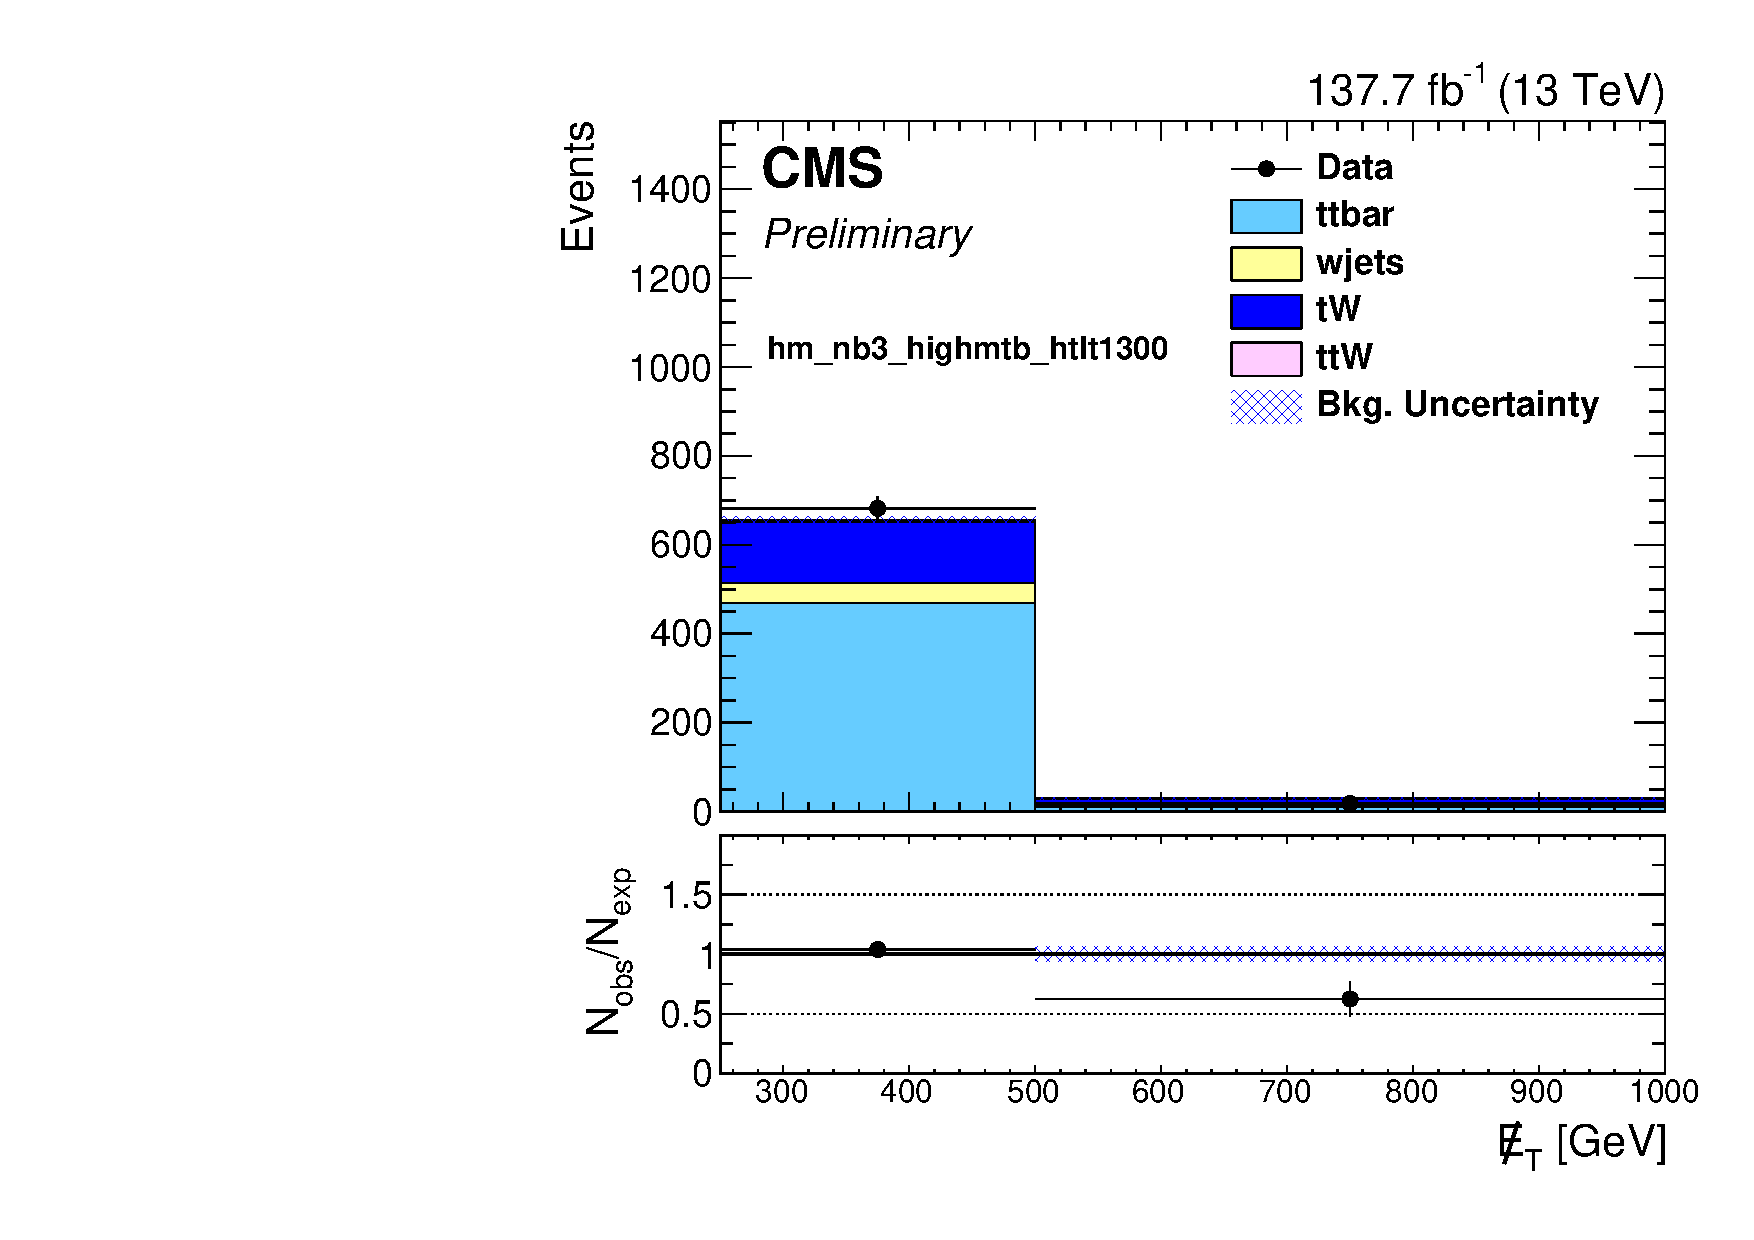
\includegraphics[width=0.32\textwidth]{../Research/SUSY/2019/LLB/lepcr_allEras/MET_pt_DataMC_hm_nb3_highmtb_nt0_nrt2_nw0_htlt1300__.pdf} 
  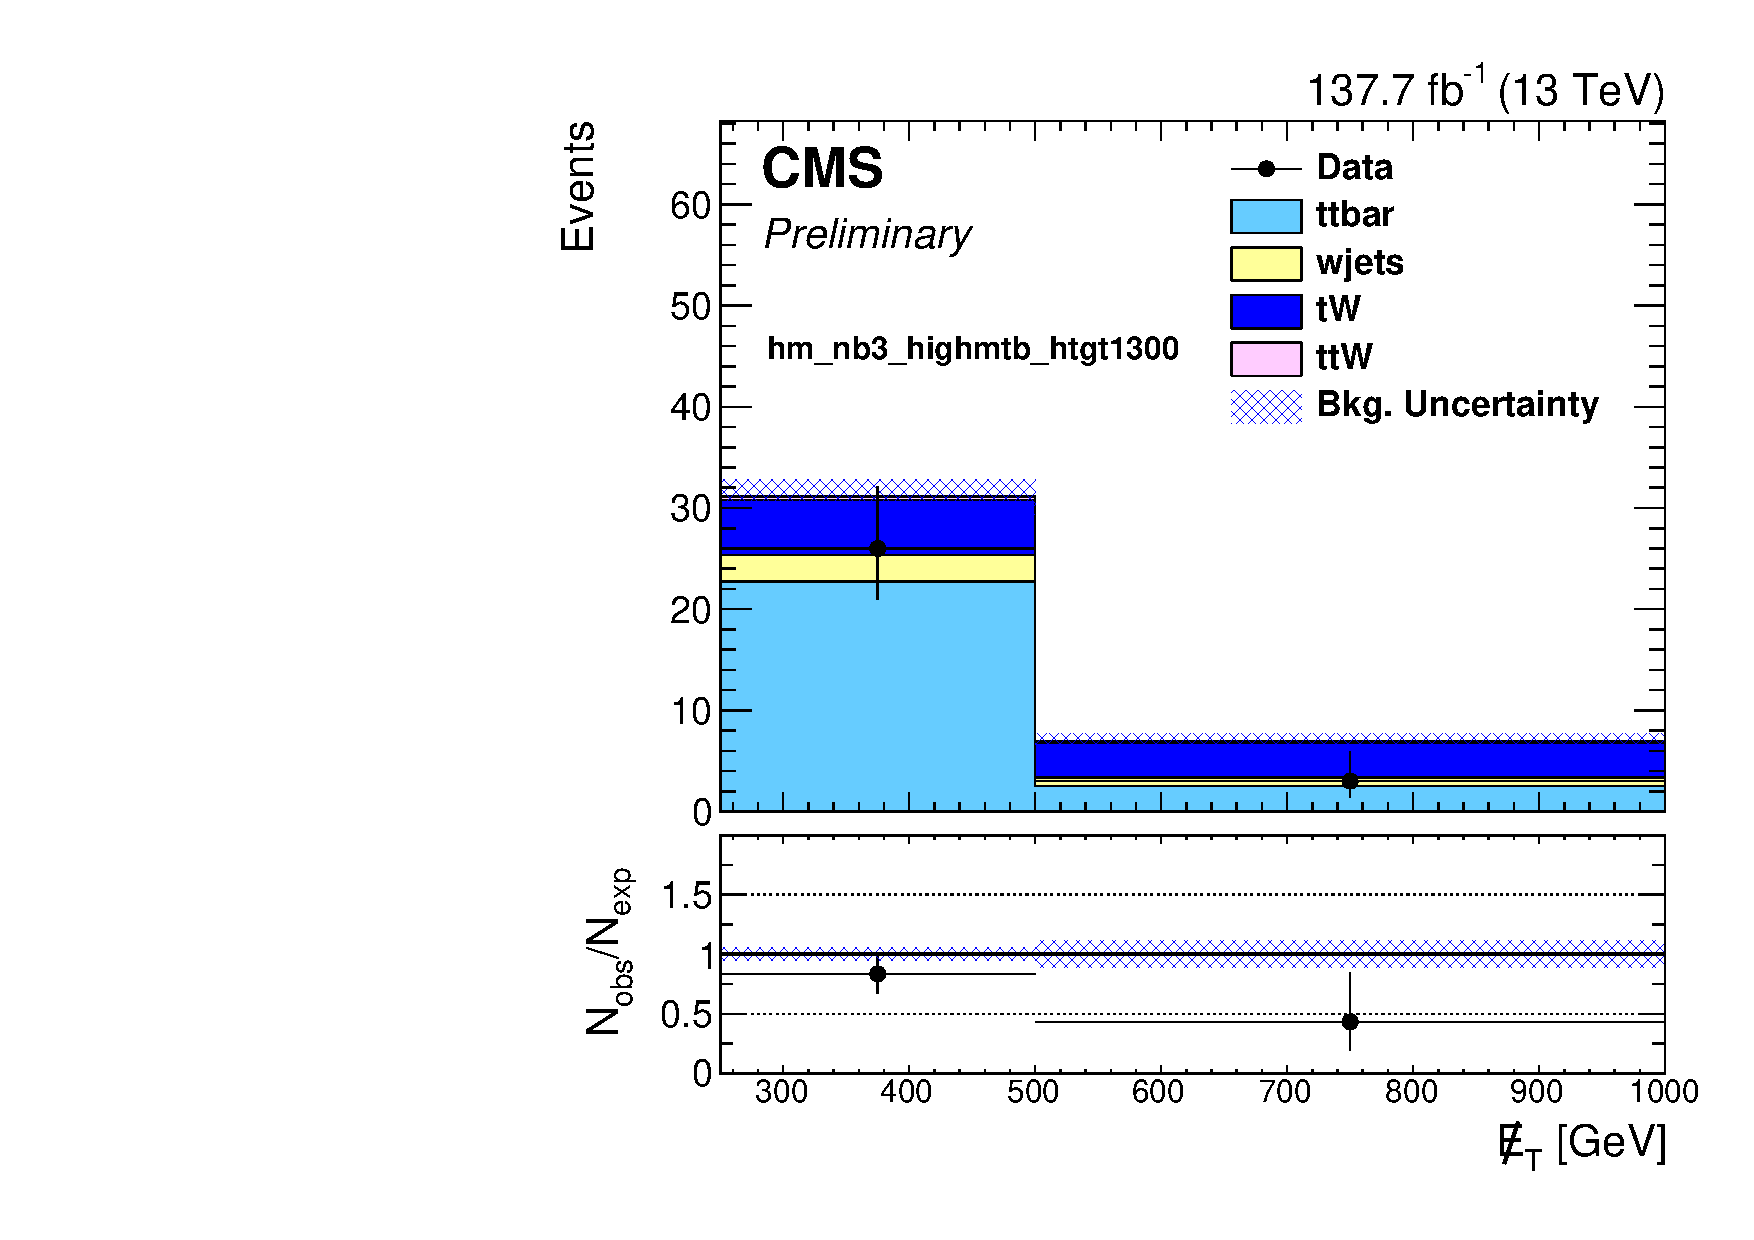
\includegraphics[width=0.32\textwidth]{../Research/SUSY/2019/LLB/lepcr_allEras/MET_pt_DataMC_hm_nb3_highmtb_nt0_nrt2_nw0_htgt1300__.pdf} 
  \includegraphics[width=0.32\textwidth]{../Research/SUSY/2019/LLB/lepcr_allEras/MET_pt_DataMC_hm_nb3_highmtb_nrtntnwgeq3__.pdf} \\
	\end{center}
	\caption{Comparison of the \met~distribution in the single-lepton sample after applying the high \dm~baseline selection in the $\nb\geq3$ $\nt=2, \nrt=2,$ or $\nw=2$ region. Data and simulation are represented by the black points and stacked histograms, respectively. The error bars on the ratio of observed data to simulation correspo    nd to the data statistical uncertainty and the shaded blue band represents the statistical uncertainty on the simulation. These regions are included with the search regions in the simultaneous fit for the signal extraction in order to estimate the LL contribution.
	 %               The plots in the top row are for events with $\mtb<175$~\GeV, with $5\leq\nj<7$ on the left and $\nj\geq7$ on the right. 
	 %               The plots in the middle row are for events with $\mtb>175$~\GeV and $\nt=0, \nw=0$, with $5\leq\nj<7$ on the left and $\nj\geq7$ on the right. 
	 %               The plot in the bottom row is for events with $\mtb>175$~\GeV and $\nj\geq5$, with $\nt=0, \nw\geq1$ on the left, $\nt\geq1, \nw=0$ on the middle, and $\nt\geq1$, and $\nw\geq1$ on the right.
	 }
	\label{fig:llb-1lcr-datavsmc-hm-nb3-2}
\end{figure}
